\documentclass[a4paper]{article}

%% Language and font encodings
\usepackage[english]{babel}
\usepackage[utf8x]{inputenc}
\usepackage[T1]{fontenc}

%% Sets page size and margins
\usepackage[a4paper,top=3cm,bottom=2cm,left=3cm,right=3cm,marginparwidth=1.75cm]{geometry}

%% Useful packages
\usepackage{amsmath}
\usepackage{graphicx}
\usepackage[colorinlistoftodos]{todonotes}
\usepackage[colorlinks=true, allcolors=blue]{hyperref}
\usepackage{subfigure}
\usepackage{soul} % strikethrough

\title{Why deconvolve Ca\textsuperscript{2+}?}
\author{Mathew H. Evans}

\begin{document}
\maketitle

\begin{abstract}
Two-photon fluorescence imaging of somatic calcium (Ca\textsuperscript{2+} for short) is an increasingly popular technique for recording the activity of large groups of neurons (cite reviews). Given that Ca\textsuperscript{2+} is an indirect measurement of neural activity, and signal quality considerations (background noise, slow kinetics, and heterogeneity in expression across cells) the fluorescence time-series is typically \emph{deconvolved} prior to tuning or correlation analysis. Recent efforts have seen an explosion in the number of available methods for Ca\textsuperscript{2+} deconvolution (AKA spike inference), with impressive results (Theis, spikefinder). Here we reconsider this progress showing (i) a popular metric - Pearson correlation coefficient (PCC) - is poorly conditioned (results change a great deal with small changes in parameters), and results in poor estimates of firing rates (see also Ganmor, Reynolds CosMIC), (ii) when applied to data collected at large-scale-recording resolution (with sampling rates of 2-10Hz) performance is inconsistent and poorer than may be expected from published results \emph{I.E. disagreement between methods (re FR, 'tuned', correlations, dimensionality), poor recovery of temporal tuning}. We conclude that the purported advantages of deconvolution may not outweigh the disadvantages of losing information and introducing noise. Great care must be taken in the application of deconvolution methods and in the interpretation of findings based on these methods.

%Some notes on our efforts to compare calcium deconvolution methods. After describing a different spike distance metric (Victor \& Purpura 1996), we outline the different deconvolution methods attempted and compare their results on ground truth and example `real' data.
\end{abstract}

\section{Introduction}
\textbf{why deconvolve} \\
- improve signal/noise ratio i.e. better estimate what the cell is doing\\
- increase temporal resolution e.g. to recover tuning and correlations\\
- normalisation of expression across neurons\\


\noindent \textbf{how to deconvolve}\\
- many methods giving different results (due to analysis/design choices)\\
- comparing methods involves metrics\\
- metrics are important as they give different results\\

\noindent \textbf{the cautionary tale}\\
- if the signal isn't perfect our metrics and methods lead to biased estimates of neural properties (FR, tuning, correlations)\\
- this bias may be worse than the benefits we're supposed to get when deconvolving \\
- artefacts may not be removed after all\\

\newpage

\section{Results} 
\subsection*{Fitting methods using Pearson correlation coefficient leads to over-estimating firing rate}
\emph{The point of this section is that if you are going to do deconvolution, PCC is a biased metric so use something else e.g. ER. This isn't a particularly novel point any more - see Reynolds biorxiv 2017 + Ganmor}\\

\noindent \textbf{Results in brief}\\
- Using PCC as a metric leads to over-estimation (and under estimation) of firing rate\\
- PCC does not vary smoothly with model parameters, potentially leading to poor (over) fitting to training data \emph{N.B. we didn't test this - all data was used for fit + evaluation, not separate training/test sets}\\
- ER is a better choice (but see also CosMIC, Reynolds et al 2017 or Information based methods, Theis)\\
- This result is true regardless of method used (see repeated analysis on MLSpike + LZero\\
- This result is true on both high and low frame rate data\\
- TO DO - what is the single figure we need to summarise these results? What metric can we show e.g. variance, or MAD of FR estimates is larger for PCC than ER?

To assess the performance of deconvolution algorithms at estimating spike trains from Ca\textsuperscript{2+} signals, different methods can be tested on \emph{ground truth} datasets - where the spiking activity of a cell was recorded simultaneously with Ca\textsuperscript{2+} imaging, ideally using high-signal-to-noise techniques such as juxtacellular recording (see Figure \ref{fig:ground_truth_diagram}).



\begin{figure}%[h!]
\centering
\subfigure[]{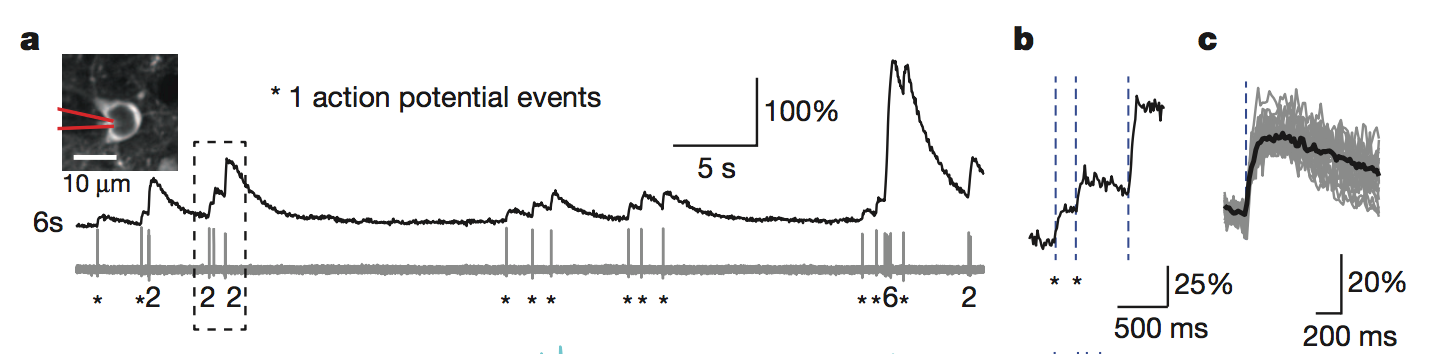
\includegraphics[trim={0 0 0 0},clip,width=0.8\textwidth]{figs/Chen_cai_F3a.png}}
\subfigure[]{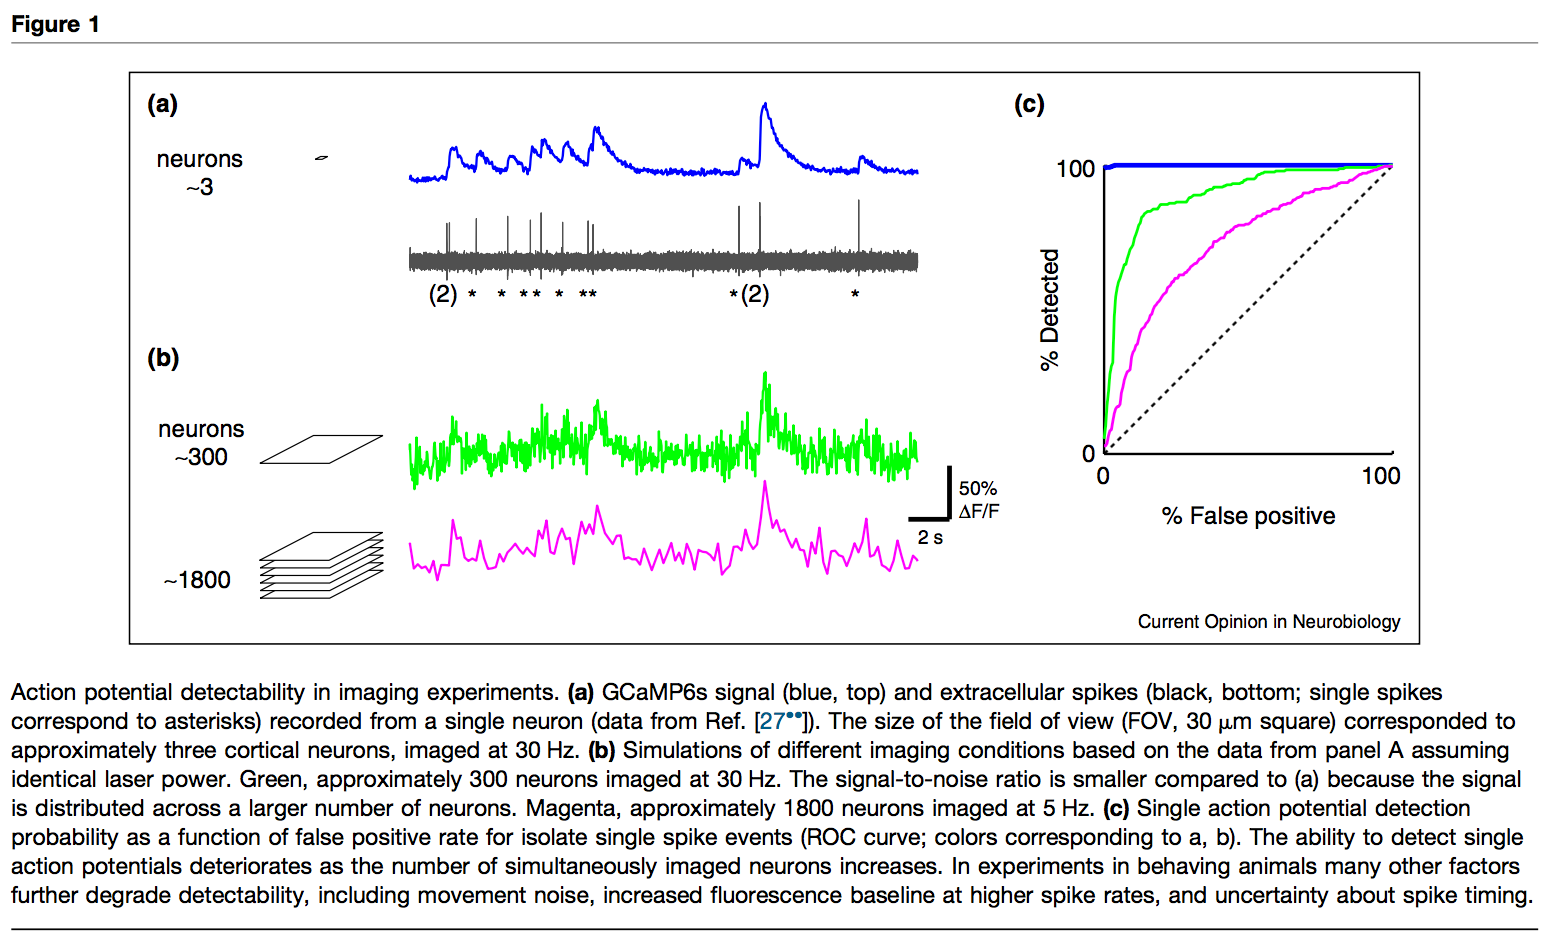
\includegraphics[trim={0 0 0 30},clip,width=0.8\textwidth]{figs/Peron_COiN_15.png}}
\caption{\label{fig:ground_truth_diagram} (a) Ground truth data collection example from Chen et al. Nature 2013. Top left, an example field of view from imaging data. Red lines denote the outline of a juxtacellular recording pipette. Time series shows measured calcium fluorescence (top) and simultaneously recorded voltage (below). Spikes are marked with asterisks. (b) Frame rate/ spatial resolution trade offs. All light microscopy experiments (including two photon imaging) have a 'photon budget' (set by the microscope and sample) which can be deployed by the experimenters to achieve certain goals. Higher signal to noise can be achieved with high frame rates and zoomed in imaging (more pixels per cell). If the goal is to record from large numbers of neurons the overall photon budget must be spread more thinly per neuron, with smaller numbers of pixels per cell and lower frame rates, resulting in lower signal to noise ratios (Figure reproduced from Peron, Chen \& Svoboda COiN 2015)}
\end{figure}

Figure \ref{fig:deconv_metrics1} (b) shows the results from decorrelating ground truth datasets using Suite2P (Pachitariu et al) using a range of a threshold parameter which trades off misses vs false detections. In general PCC increases as estimated firing rate increases. However, this can lead to overestimation of the true firing rate, when comparing the true firing rate to the estimated firing rate using the `best' (highest PCC) parameters (blue dots in Figure \ref{fig:deconv_metrics1} (d,e)). Another downside of PCC as a metric is it does not change smoothly with parameter changes, as can be seen in the lines for individual cells in Figure \ref{fig:deconv_metrics1} (b).

To address the weaknesses of PCC, we implemented the Error Rate (ER) spike distance metric of Deneaux et al 2016, a summary measure based on the distance measure of Victor \& Purpura (1996). ER (described in Figure \ref{fig:deconv_metrics1} (a)) returns a normalised score which is 0 for a perfect match, and 1 when all the spikes are missed. When applied to deconvolution of ground truth data, ER is `best' (lowest) for intermediate estimated firing rates, suggesting that estimates closer to the true firing rate are rewarded with good scores (Figure \ref{fig:deconv_metrics1} (c)). This intuition is shown to be true when comparing the best estimate of firing rate to the true firing rate for each cell (green dots in Figure \ref{fig:deconv_metrics1} (d,e)). Over the population PCC overestimates firing rate, in some cases severely (Figure \ref{fig:deconv_metrics1} (d,e)). Though ER also overestimates firing rate, it does so to a much smaller degree (mean error $\sim$0.1Hz). In addition, unlike for PCC, individual cell results in Figure \ref{fig:deconv_metrics1} (c) show ER varies smoothly with deconvolution parameters. These results are true if other deconvolution algorithms are used (Figures \ref{fig:deconv_metrics_MLSpike} and \ref{fig:deconv_metrics_LZero})

Large scale Ca\textsuperscript{2+} imaging experiments are optimised to record from many neurons at once, and typically use lower frame rates and fewer pixels per cell than the ground truth experiments described above (Figure \ref{fig:ground_truth_diagram} (b)). Therefore it is important to ask whether the problems of using PCC as a metric are alleviated or compounded in a low frame rate regime. To assess this we repeated the analysis of Figure \ref{fig:deconv_metrics1}  with ground truth imaging data down sampled to 7Hz and found similar results (Figures \ref{fig:deconv_metrics_ds}, \ref{fig:deconv_metrics_MLSpike} and \ref{fig:deconv_metrics_LZero}).

In summary, when optimising or comparing spike inference methods the choice of metric is critical. PCC is a poor choice of metric as it returns inconsistent results with small changes in algorithm parameters, and is biased towards both over and underestimation of firing rates when used across methods and sampling rates.



%\st{TO DO: add a results for other methods to Fig 1 (e).
%Also - important re application to large-scale imaging like Peron - repeat the analysis using degraded data (lower sampling rate to 7Hz in the first instance).}


\begin{figure}%[h!]
\centering
\subfigure[]{\includegraphics[trim={50 105 40 170},clip,width=0.7\textwidth]{figs/VP96_D16.pdf}}
\subfigure[]{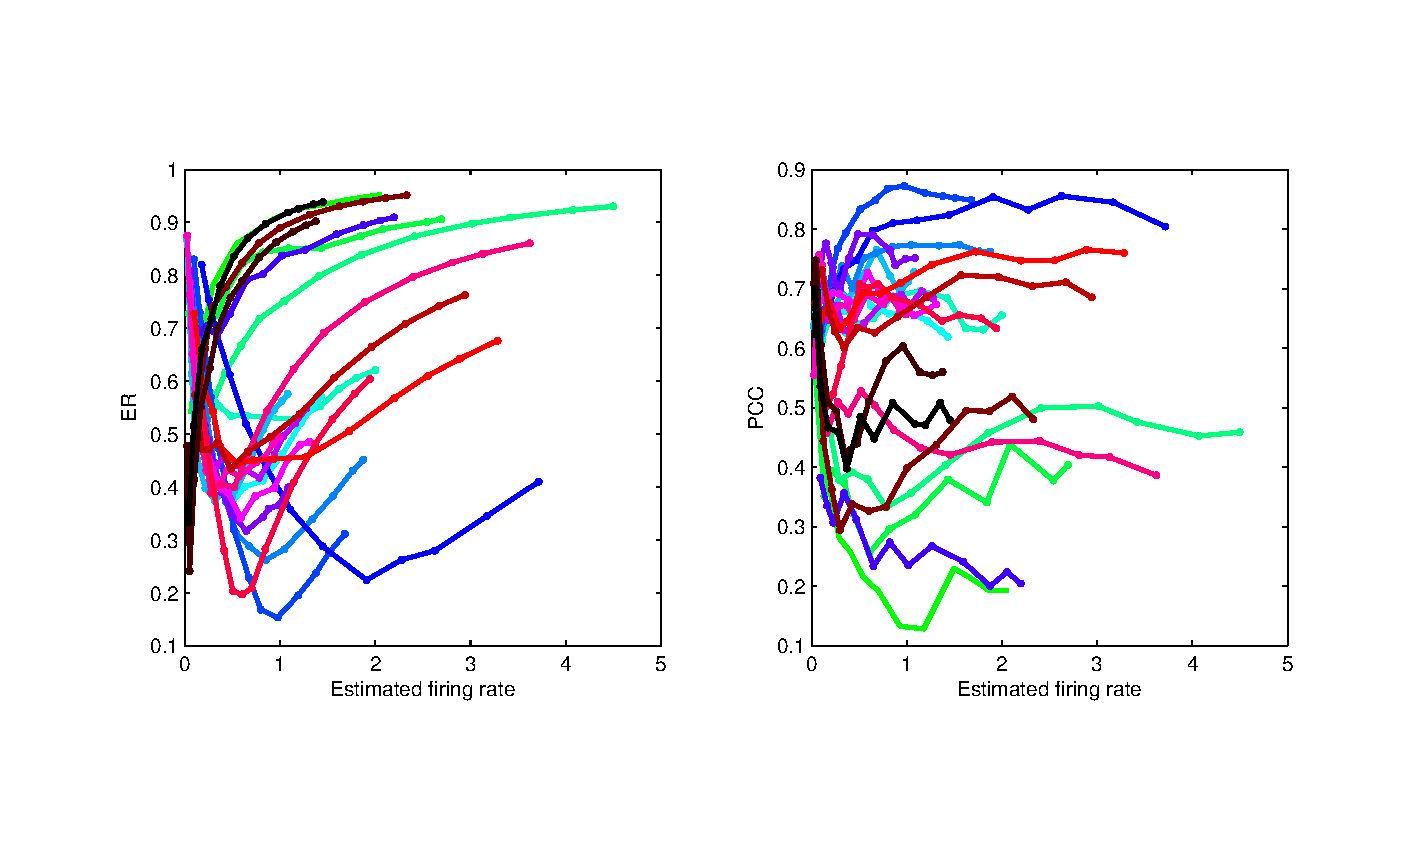
\includegraphics[trim={350 70 50 75},clip,width=0.4\textwidth]{figs/ER_PCC_FR.pdf}}%
\subfigure[]{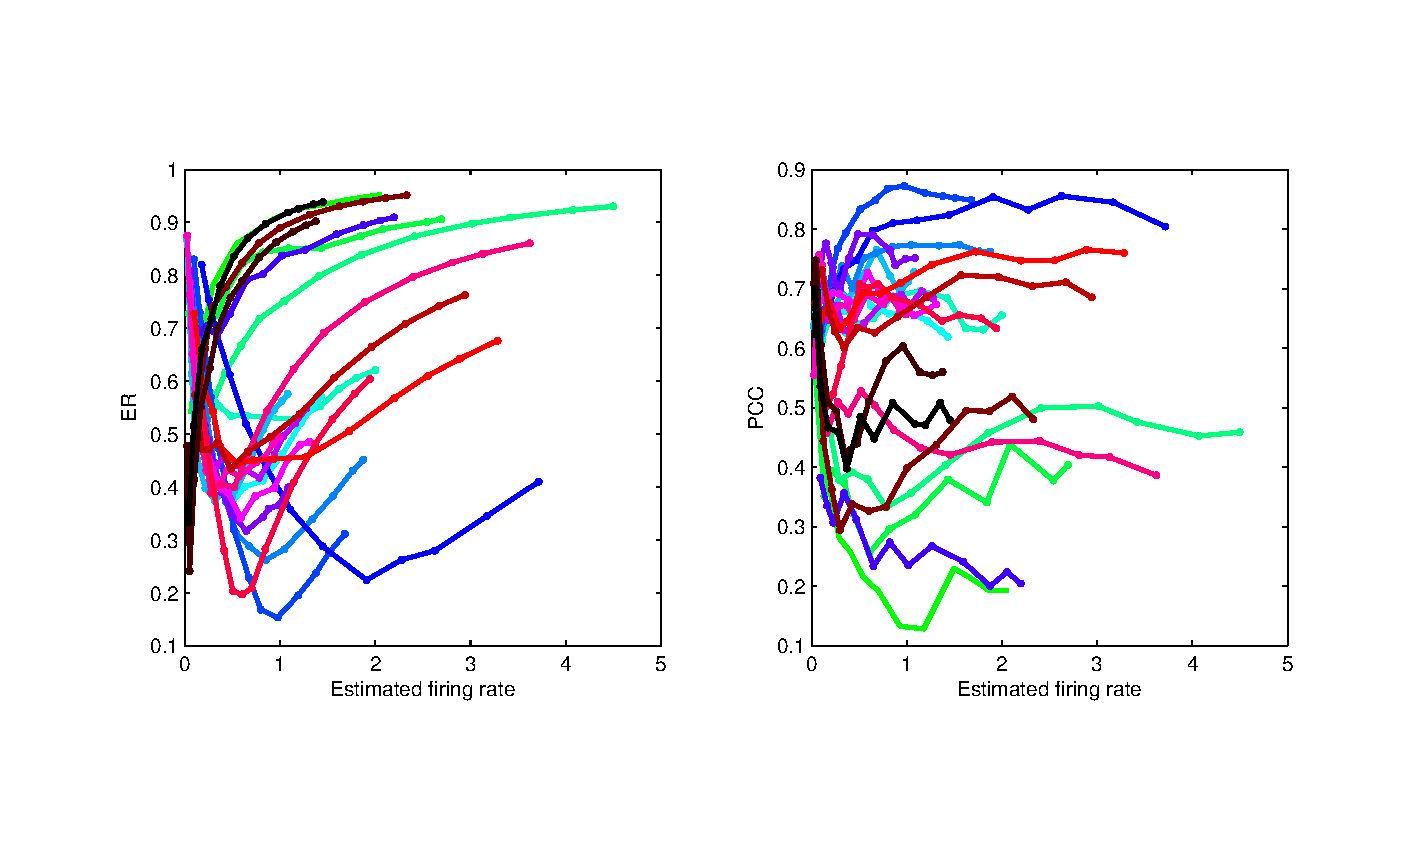
\includegraphics[trim={50 70 350 75},clip,width=0.4\textwidth]{figs/ER_PCC_FR.pdf}}
\subfigure[]{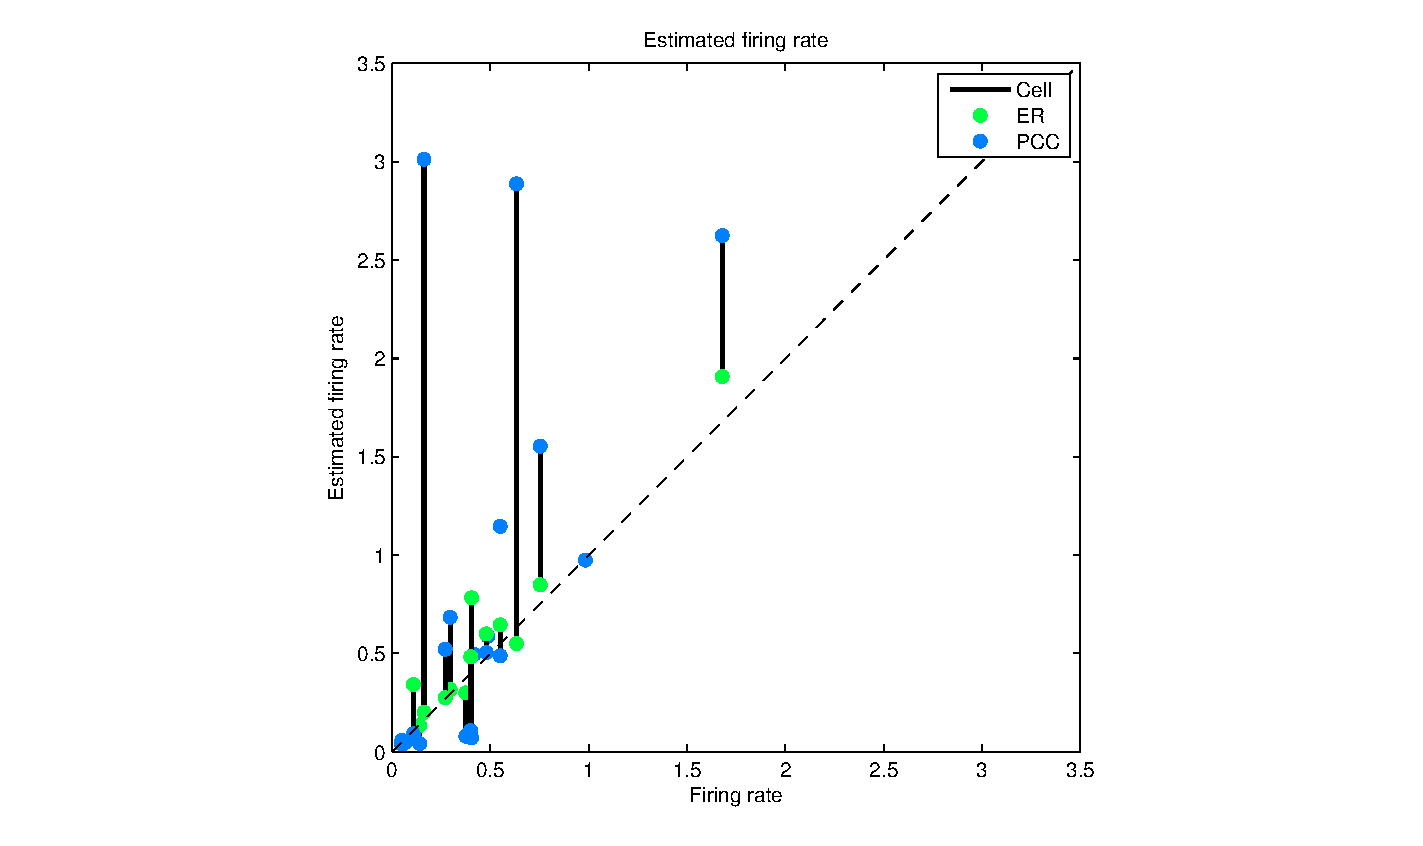
\includegraphics[trim={150 18 150 25},clip,width=0.4\textwidth]{figs/ER_PCC_FR_compare.pdf}}%
\subfigure[]{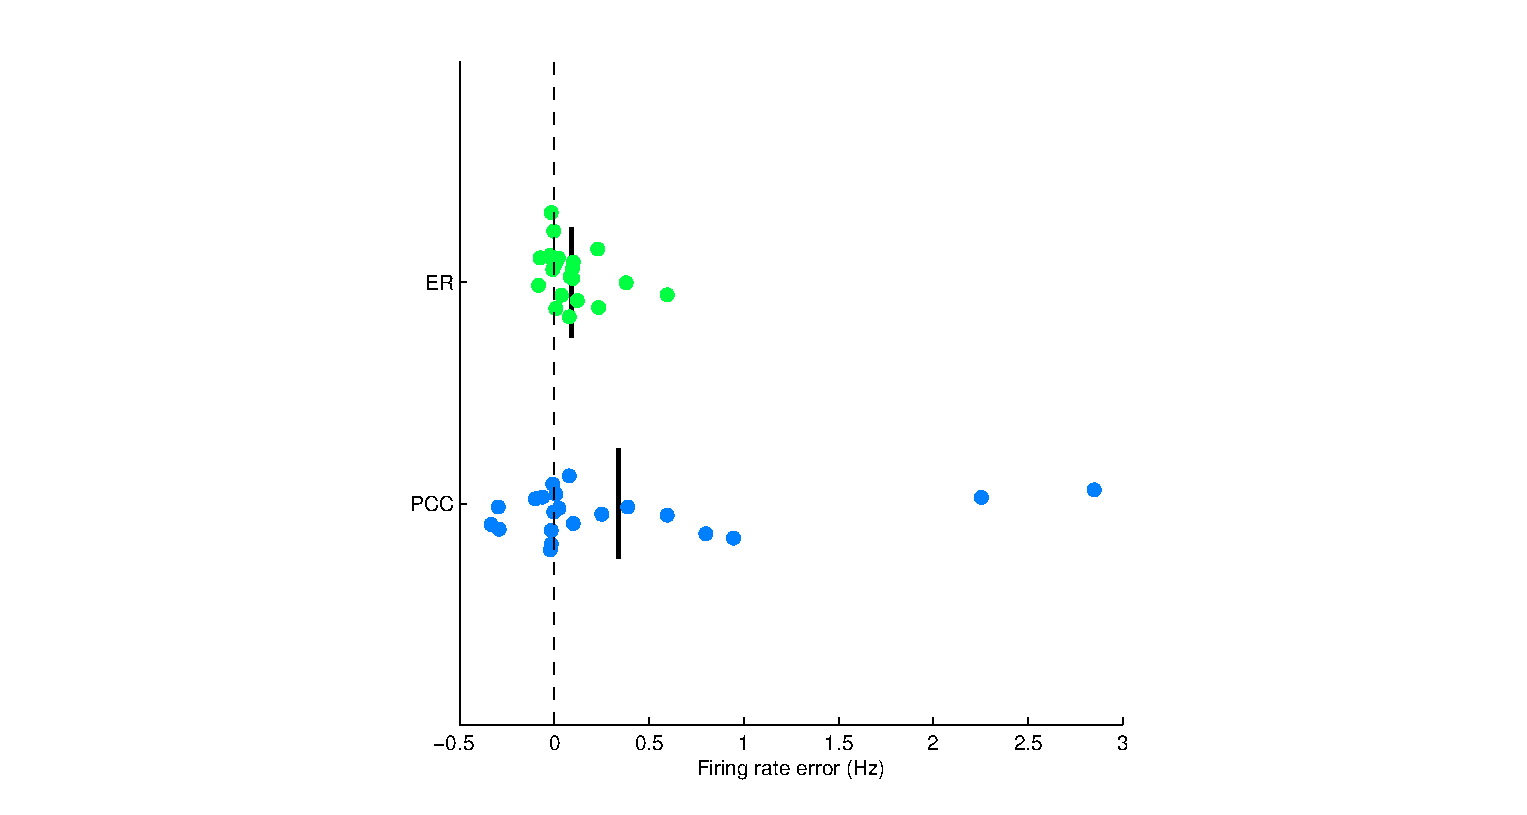
\includegraphics[trim={180 18 190 25},clip,width=0.4\textwidth]{figs/stripe_PCC_ER_square.pdf}}
% \subfigure[]{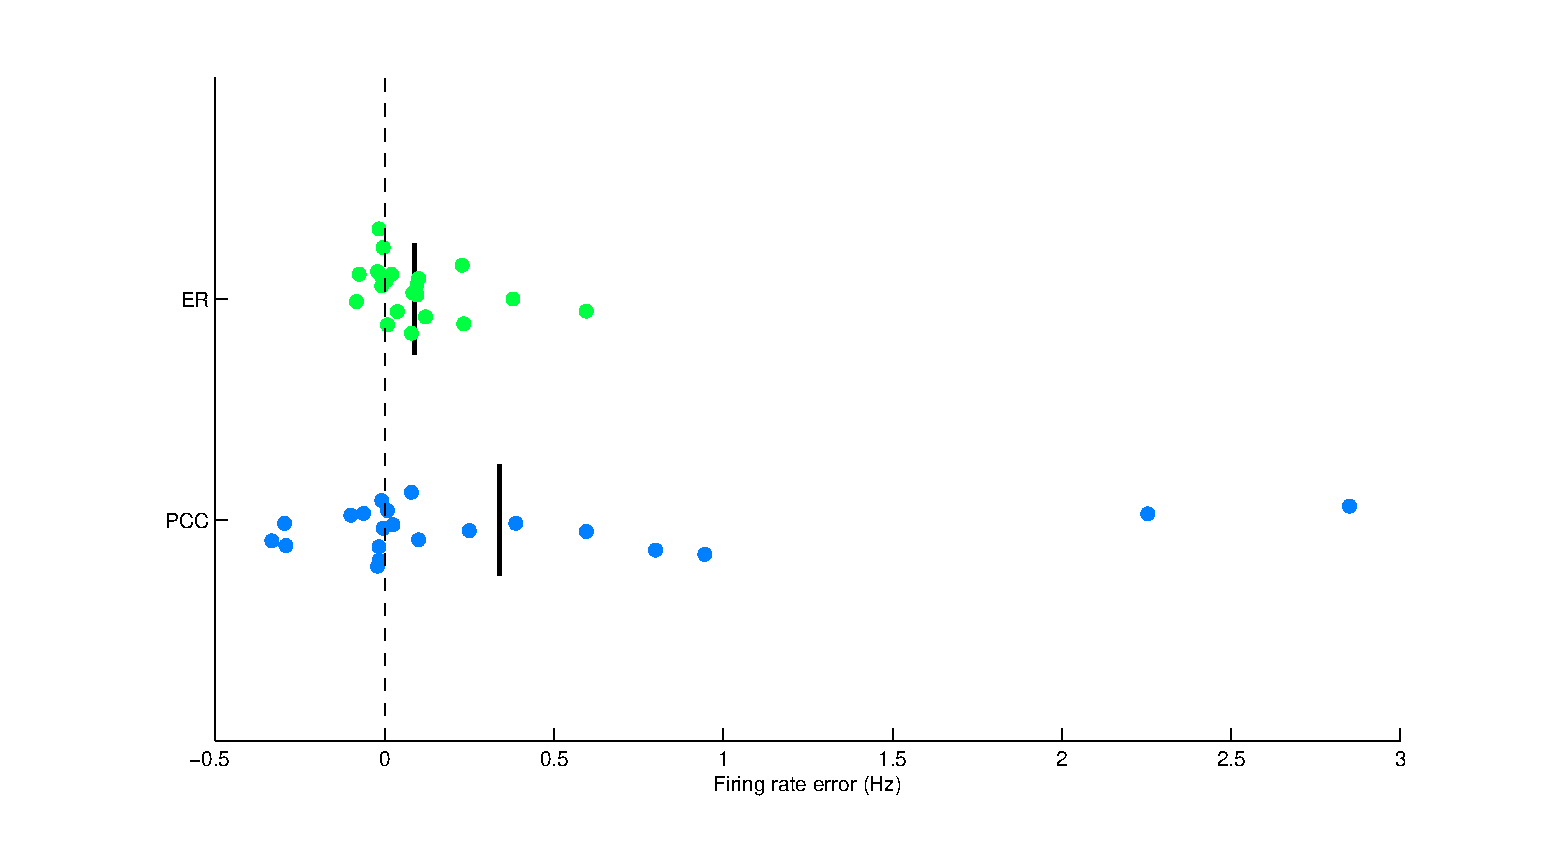
\includegraphics[trim={50 18 50 50},clip,width=0.4\textwidth]{stripe_PCC_ER.eps}}
\caption{\label{fig:deconv_metrics1} Differences in spike metrics. (a) Left: ER. Victor and Purpura (1996) proposed a spike metric to compare spike trains. This metric is generated by determining the number of elementary operations (shift, addition, or deletion of individual spikes - depicted as rows in here) required to match two spike trains, up to some temporal precision (here 0.5s). Right: In Deneaux et al 2016 the Error Rate (ER) is similarly computed as a normalised ratio of sensitivity vs precision in spike detection. Detections are counted to within 0.5s. 
(b) PCC as a function of estimated firing rate (using Suite2P, Pachitariu et al 2017). As deconvolution parameters are changed to incrementally increase the estimated firing rate - to trade off hits at the cost of false positive errors - PCC continues to improve. (c) In contrast, ER is penalised for overestimating firing rate leading to local minima. Comparing (b) and (c) ER changes smoothly with gradual changes in deconvolution parameters, whereas PCC is more stochastic, leading to noisy estimates of the best parameters. Colours are different cells. (d) Estimated firing rate for `best' deconvolution parameters versus real firing rate. Best parameters are taken as the lowest or highest points in (b) and (c), respectively. (e) Firing rate error (estimated FR - true FR). PCC both over and underestimates firing rate. ER also overestimates firing rate but to a lesser degree. Lines are means.}
\end{figure}






\begin{figure}%[h!]
\centering
\subfigure[]{\includegraphics[trim={310 250 35 270},clip,width=0.5\textwidth]{figs/ER_PCC_FR_ds.pdf}}%
\subfigure[]{\includegraphics[trim={30 250 310 270},clip,width=0.5\textwidth]{figs/ER_PCC_FR_ds.pdf}}
\subfigure[]{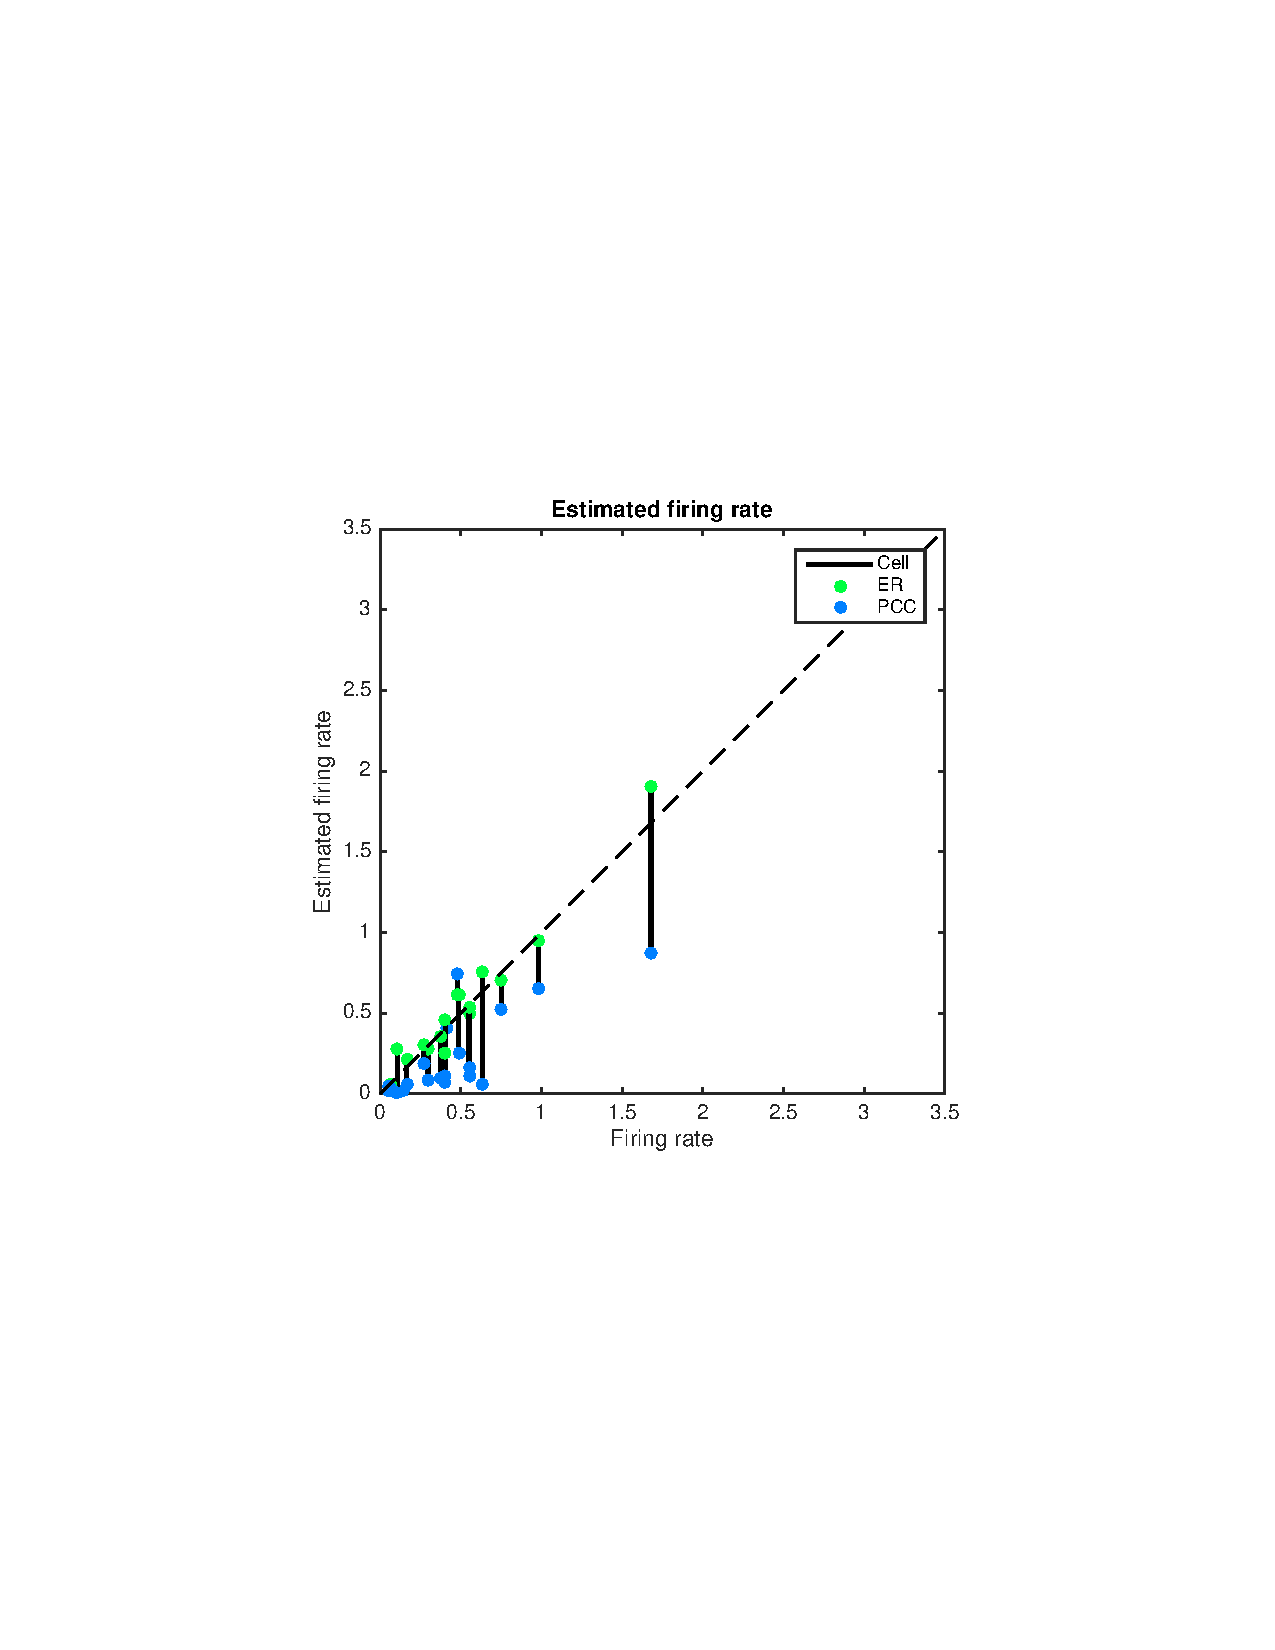
\includegraphics[trim={150 235 150 240},clip,width=0.45\textwidth]{figs/ER_PCC_FR_compare_ds.pdf}}
\subfigure[]{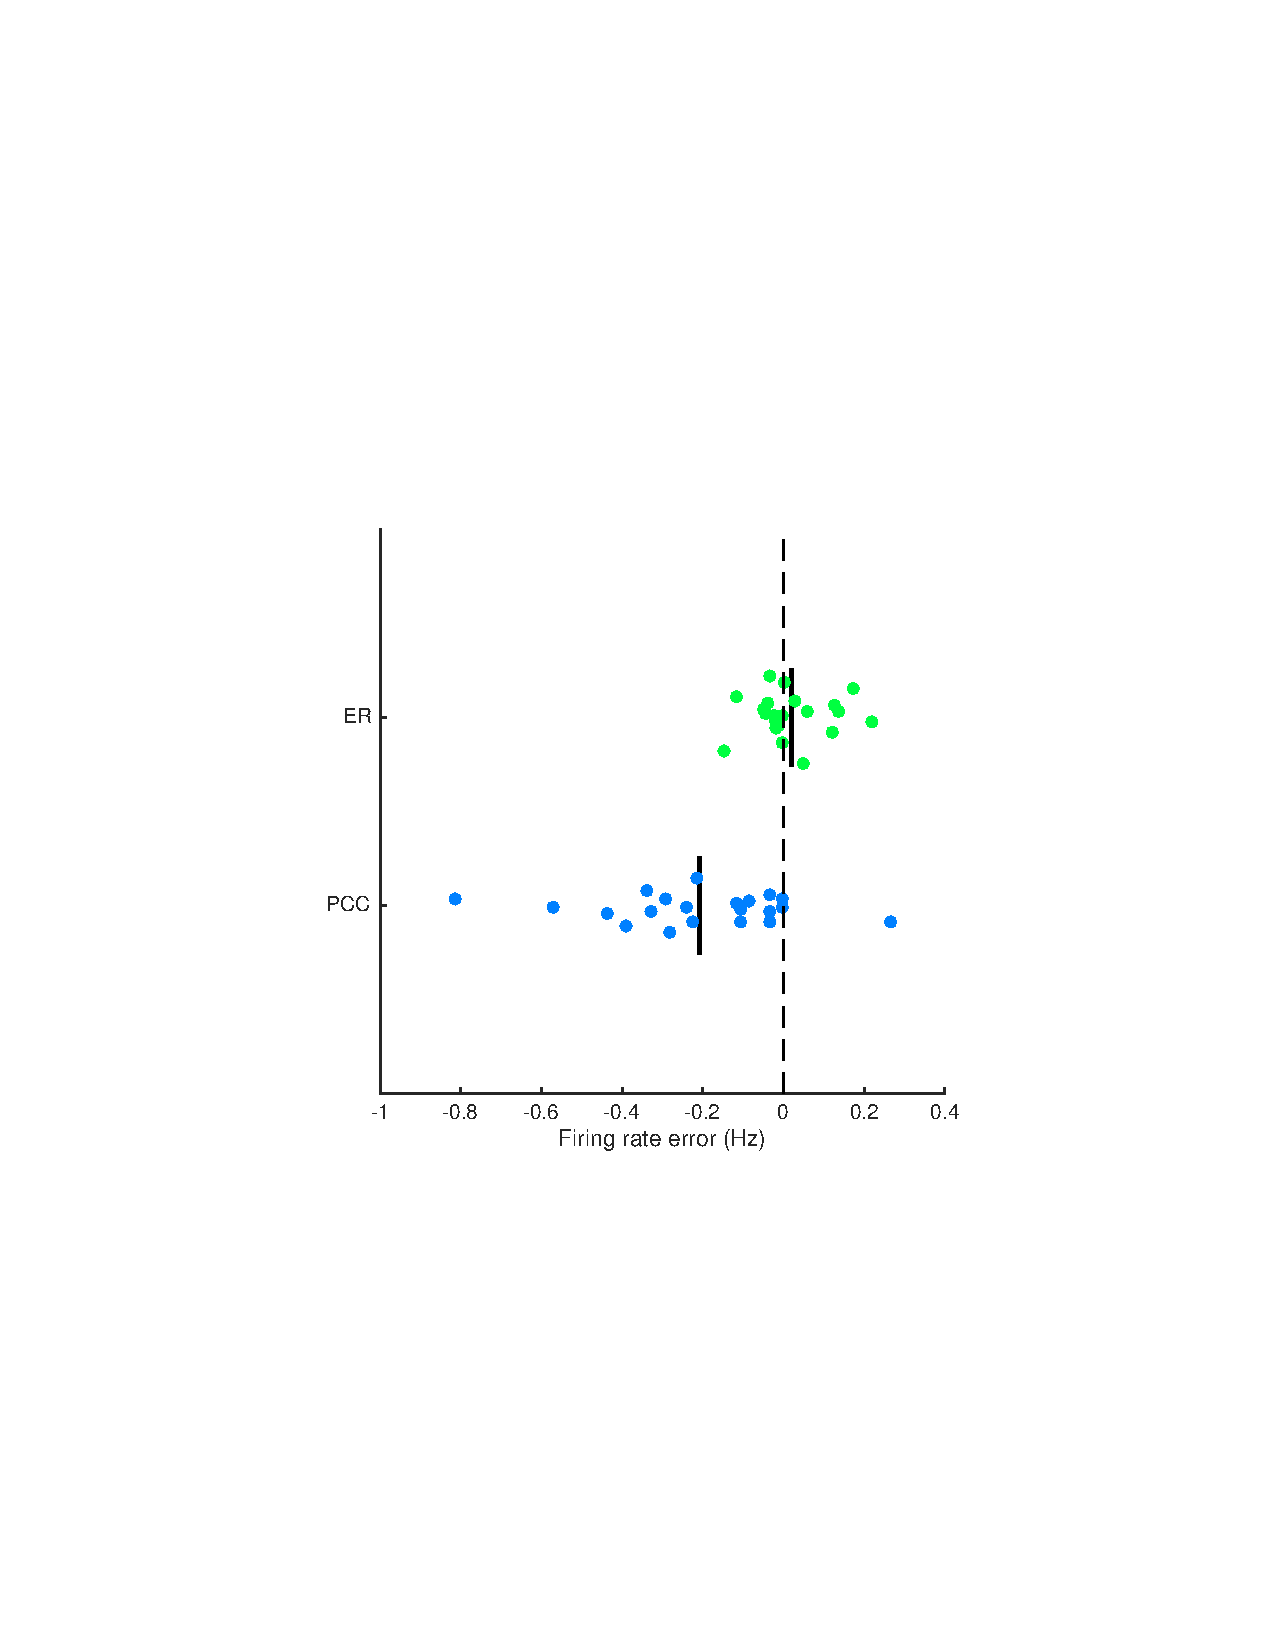
\includegraphics[trim={150 235 150 240},clip,width=0.45\textwidth]{figs/stripe_PCC_ER_square_ds.pdf}}
\caption{\label{fig:deconv_metrics_ds} Same as figure \ref{fig:deconv_metrics1} but with fluorescence data downsampled to 7Hz to mimic population imaging experiments.}
\end{figure}




\begin{figure}%[h!]
\centering
\subfigure[]{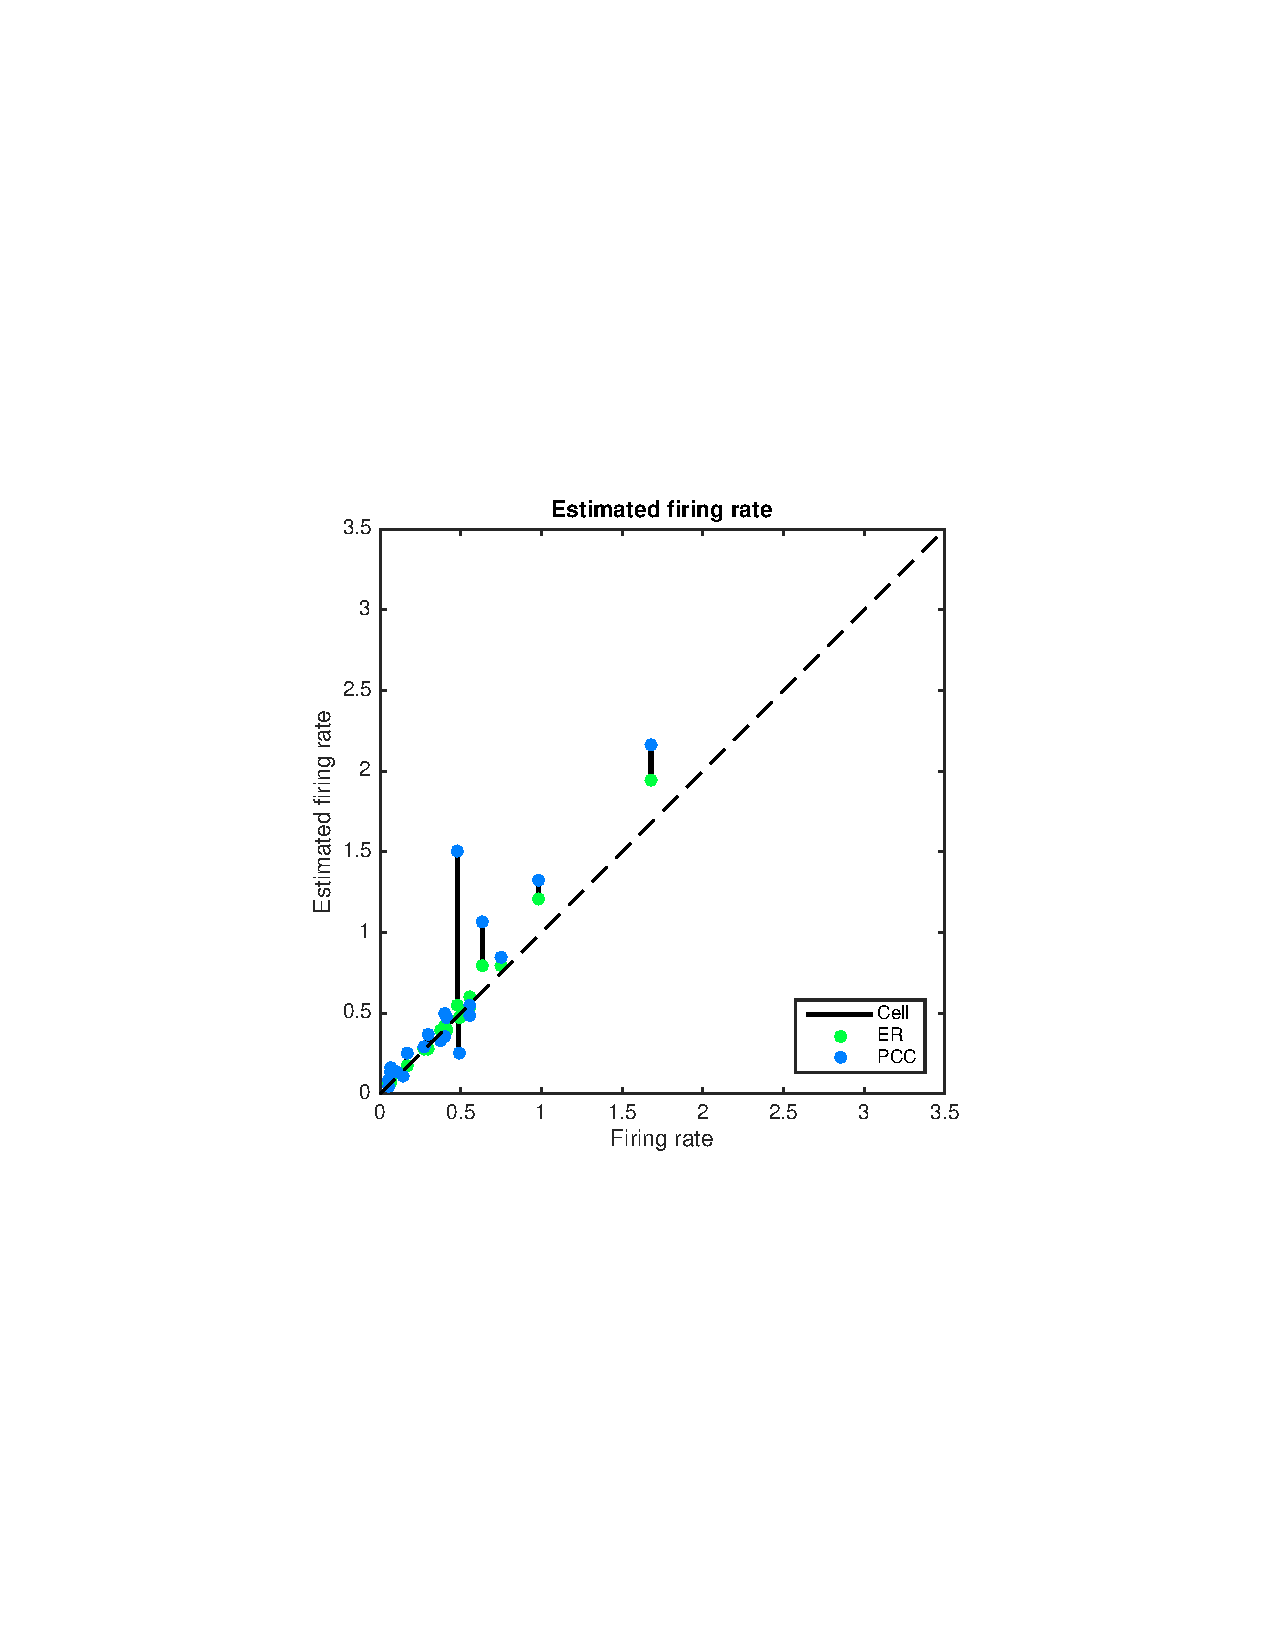
\includegraphics[trim={150 235 150 240},clip,width=0.4\textwidth]{figs/ER_PCC_FR_compare_MLSpike.pdf}}%
\subfigure[]{\includegraphics[trim={150 235 150 240},clip,width=0.4\textwidth]{figs/stripe_PCC_ER_square_MLSpike.pdf}}
\subfigure[]{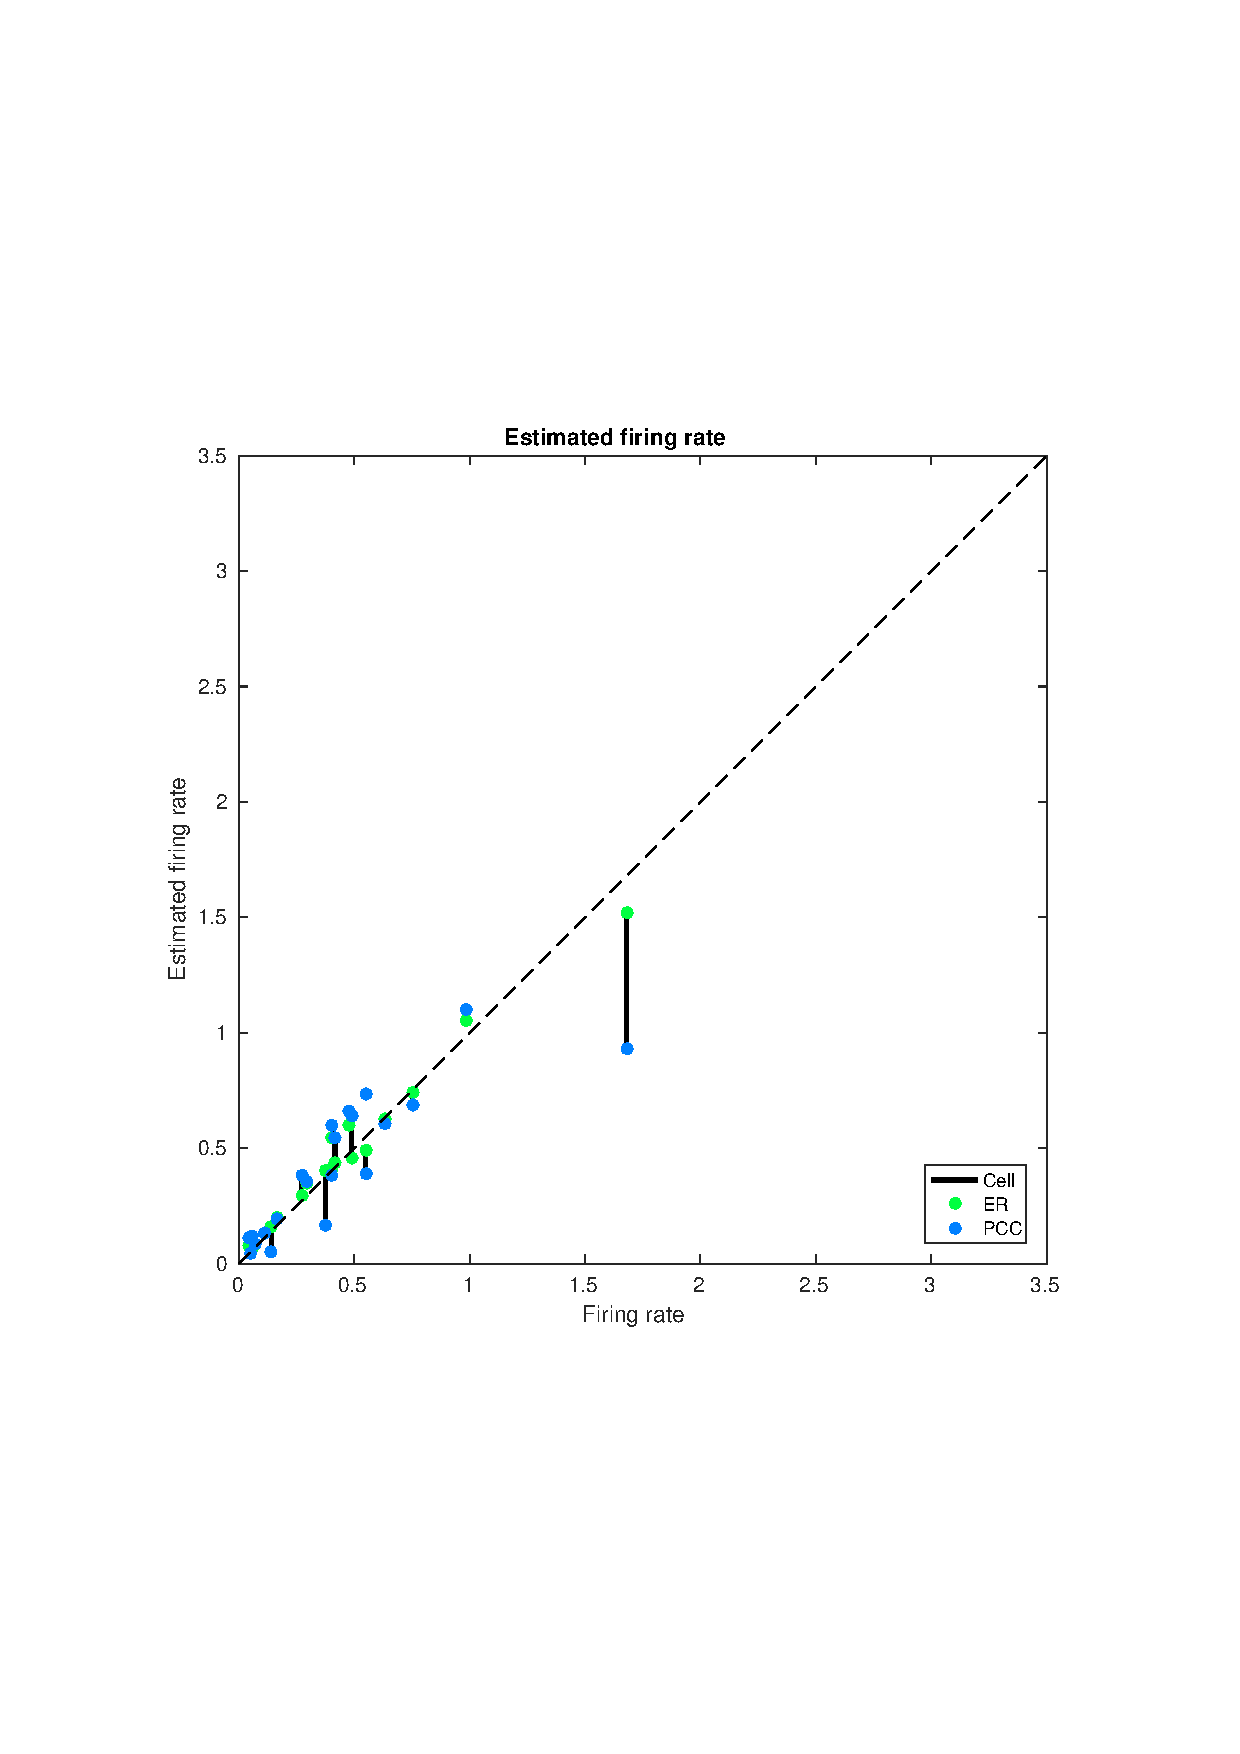
\includegraphics[trim={80 200 80 200},clip,width=0.4\textwidth]{figs/ER_PCC_FR_compare_MLSpike_ds.pdf}}%
\subfigure[]{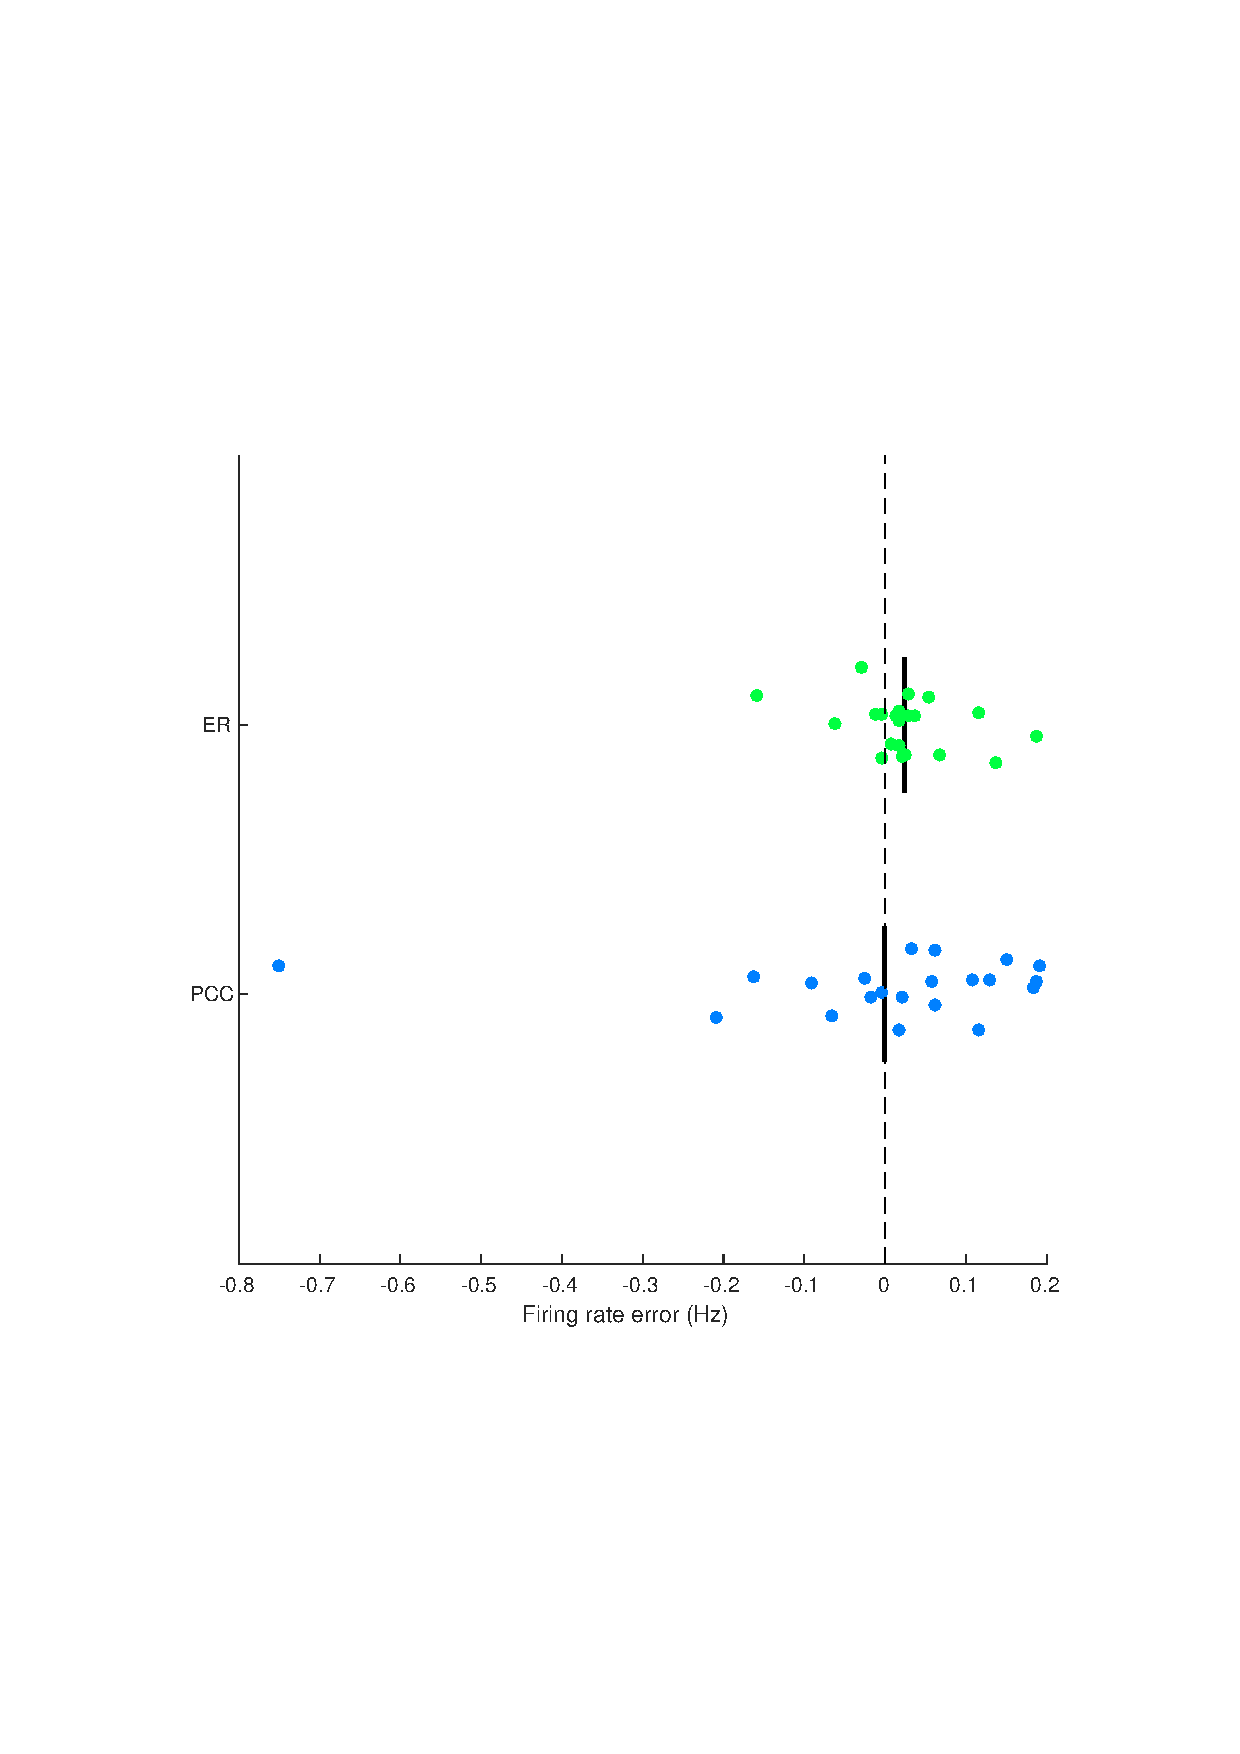
\includegraphics[trim={90 200 80 200},clip,width=0.4\textwidth]{figs/stripe_PCC_ER_square_MLSpike_ds.pdf}}
\caption{\label{fig:deconv_metrics_MLSpike} Comparing PCC and ER optimised deconvolution using MLSpike (Deneux et al 2016). (a,b) original sampling rate data. (c,d) downsampled data.}
\end{figure}


\begin{figure}%[h!]
\centering
\subfigure[]{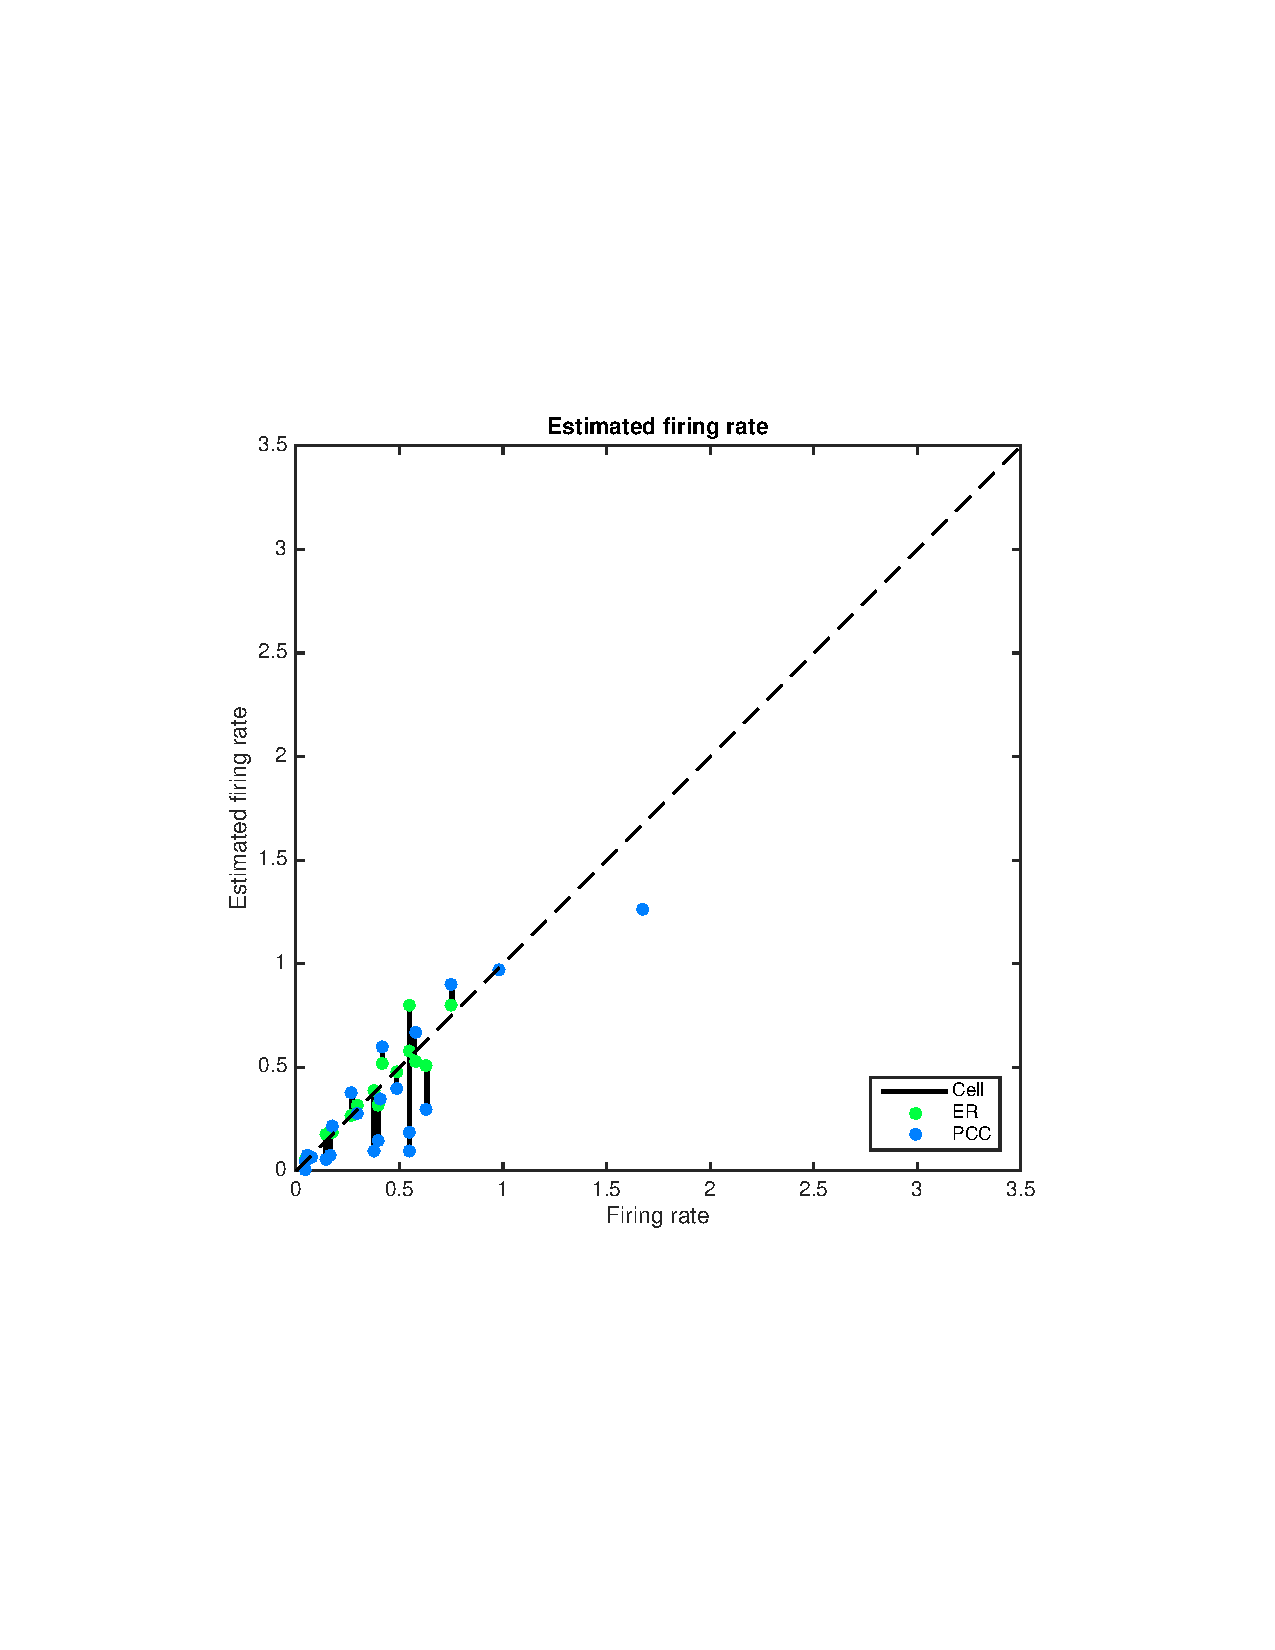
\includegraphics[trim={100 200 80 200},clip,width=0.4\textwidth]{figs/ER_PCC_FR_compare_LZero.pdf}}%
\subfigure[]{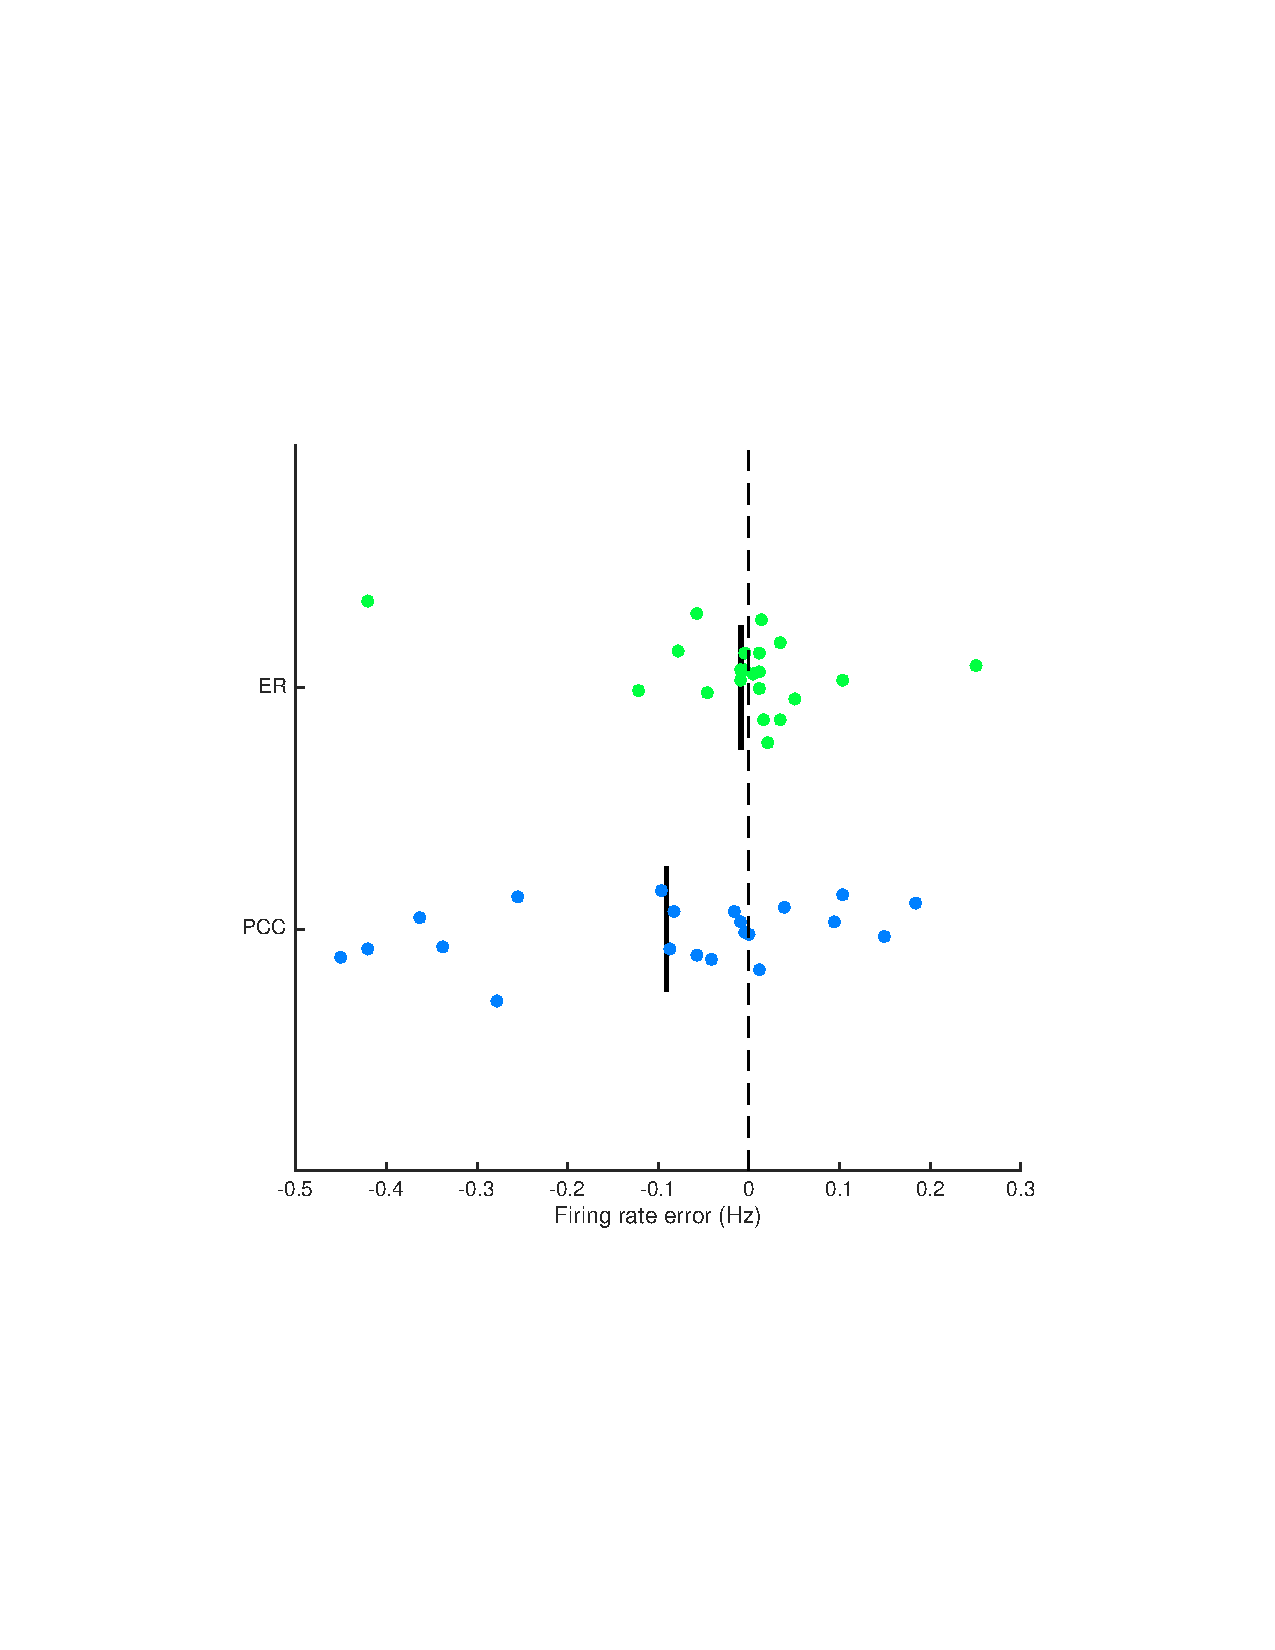
\includegraphics[trim={110 200 80 200},clip,width=0.4\textwidth]{figs/stripe_PCC_ER_square_LZero.pdf}}
\subfigure[]{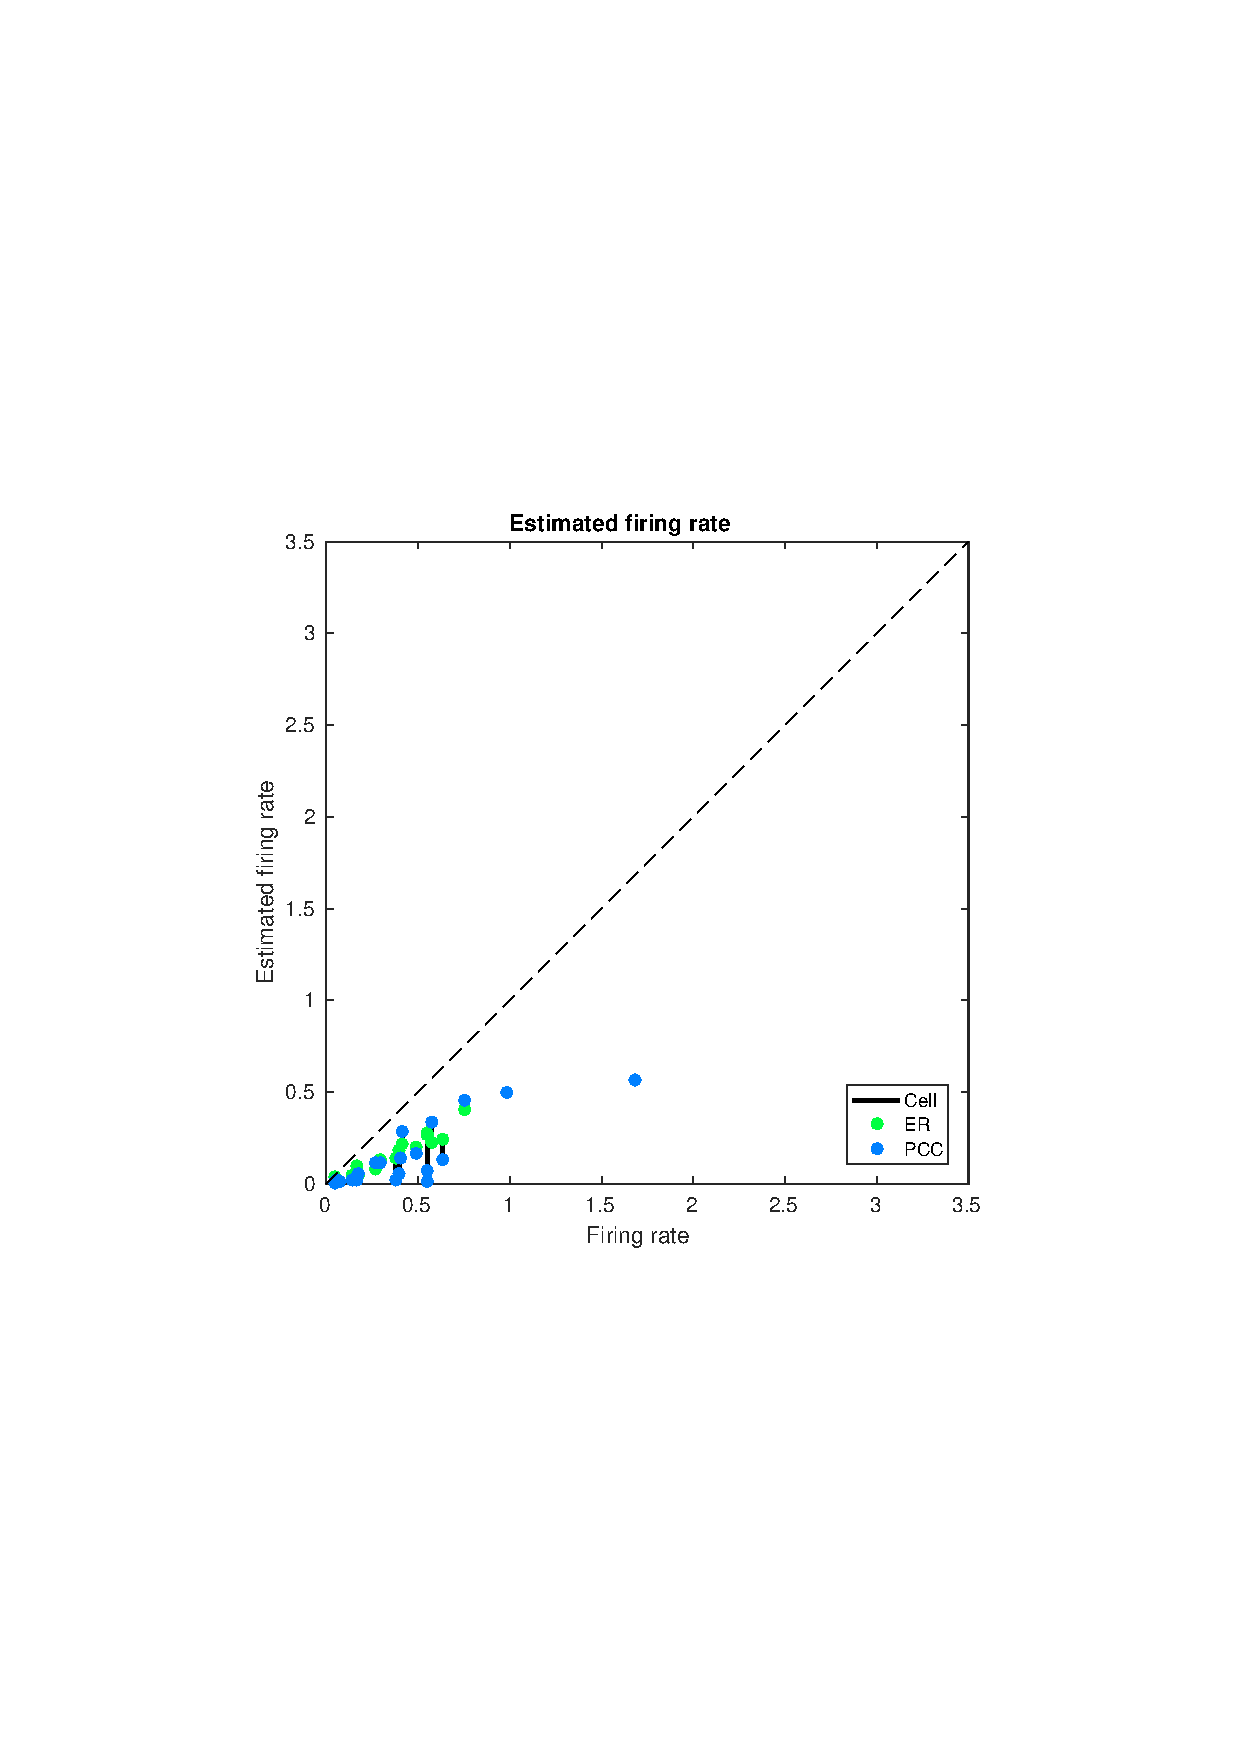
\includegraphics[trim={110 200 100 200},clip,width=0.4\textwidth]{figs/ER_PCC_FR_compare_LZero_ds.pdf}}%
\subfigure[]{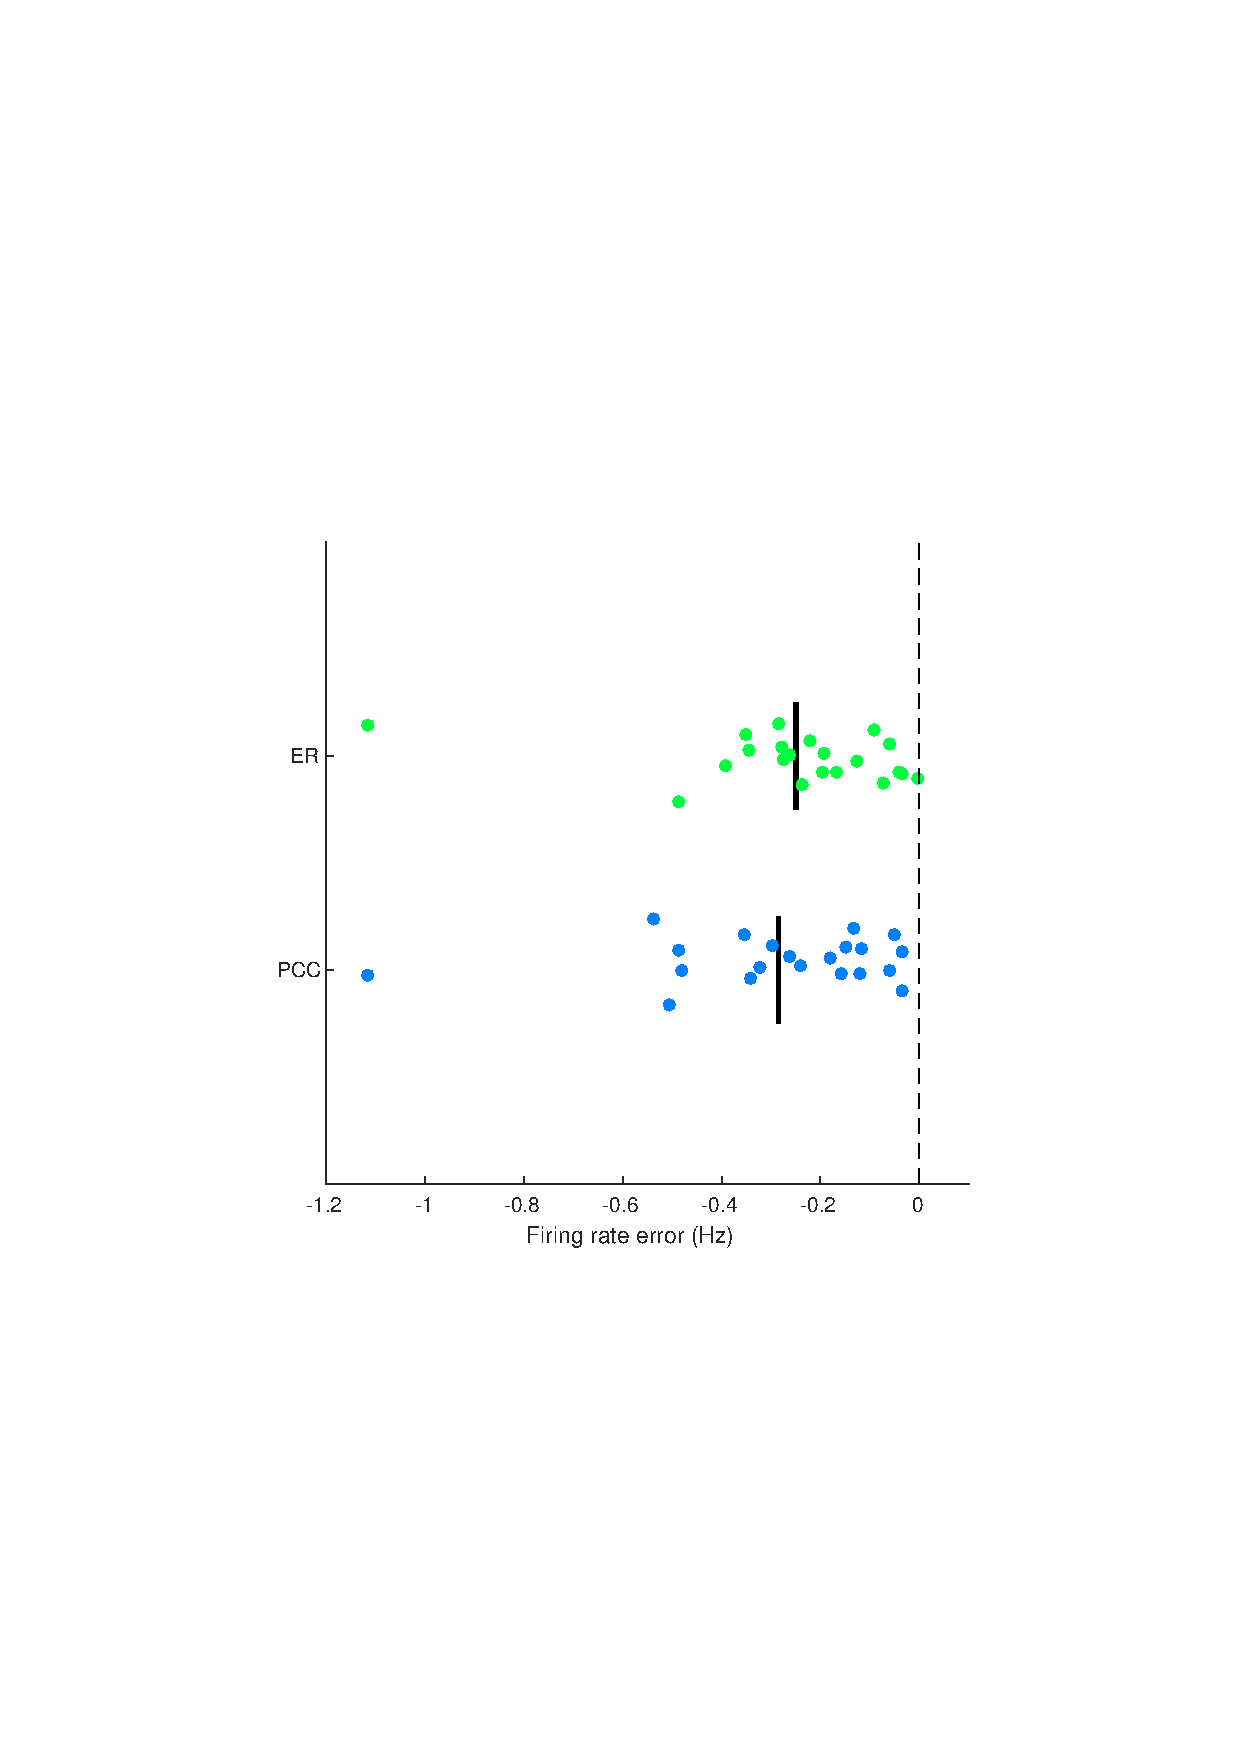
\includegraphics[trim={110 200 90 200},clip,width=0.4\textwidth]{figs/stripe_PCC_ER_square_LZero_ds.pdf}}
\caption{\label{fig:deconv_metrics_LZero} Comparing PCC and ER optimised deconvolution using LZero.(Jewell and Witten 2017). (a,b) original sampling rate data. (c,d) downsampled data.}
\end{figure}

\clearpage
\subsection{Spike inference methods lead to different estimates of simple statistics}
To determine the effect of deconvolution on simple measures of neuron activity we applied each spike inference method to data from a single experiment from Peron et al 2015 (see Figure \ref{fig:peron_setup}). In Peron et al 2015 two-photon Ca\textsuperscript{2+} imaging was used to record neural activity from up to $\sim$2000 neurons simultaneously at 7Hz from superficial barrel (Layer 2/3 somatosensory) cortex as mice performed a head-fixed tactile localisation task with their whiskers. For the results presented here 1552 neurons were recorded for a total of just over 56 minutes (23559 time points). This relatively long recording ensured good estimation of the measured parameters (see Fig. \ref{fig:supp_cxy_stability} - TO DO add similar test for firing rate estimates?).




\begin{figure}[h!]
\centering
\subfigure[]{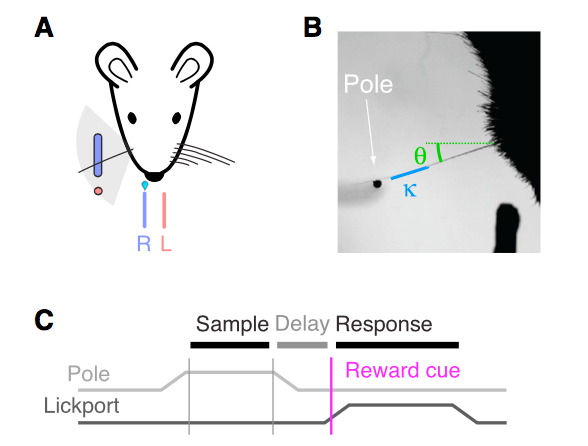
\includegraphics[trim={0 0 0 0},clip,width=0.4\textwidth]{figs/Peron_F1.png}}%
\subfigure[]{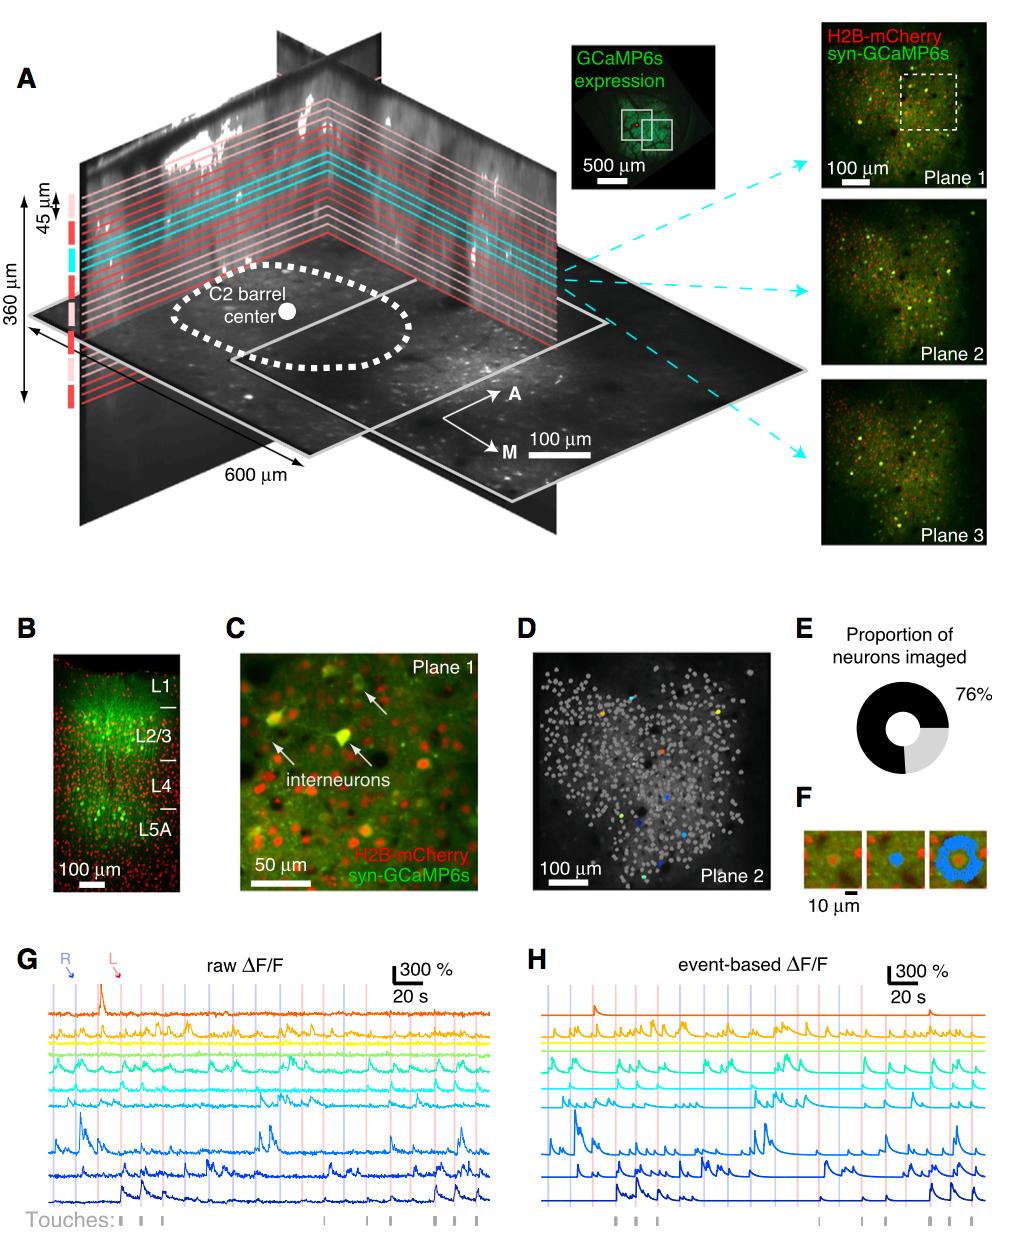
\includegraphics[trim={0 0 0 0},clip,width=0.4\textwidth]{figs/Peron_F2.png}}
\caption{\label{fig:peron_setup} Peron et al. 2015 experimental design. TO DO EXPAND description}
\end{figure}

The most basic analysis of neural activity is to determine the mean firing rate of each cell in the recording - a quantity that is known to follow a log normal distribution at the population level (Wohrer et al 2012). We determined the mean spike/event rate per cell for ten different approaches to Ca\textsuperscript{2+} deconvolution (see Methods). Figure \ref{fig:event_detection} (a) and (b) show that no two methods return the same distribution of spike/event rates. 

It has been estimated that $\sim$13\% of neocortical cells are silent (fewer than one spike every two minutes), a quantity increasing to $\sim$26\% in Layer 2/3. For the ten approaches we tested, eight estimated the proportion of silent cells to be below 1\%, with wide disagreement between the other two methods (Figure \ref{fig:event_detection} (c)). 

Even for simple statistics, the choice of spike inference method results in widely different results.





\begin{figure}%[h!]
\centering
\subfigure[]{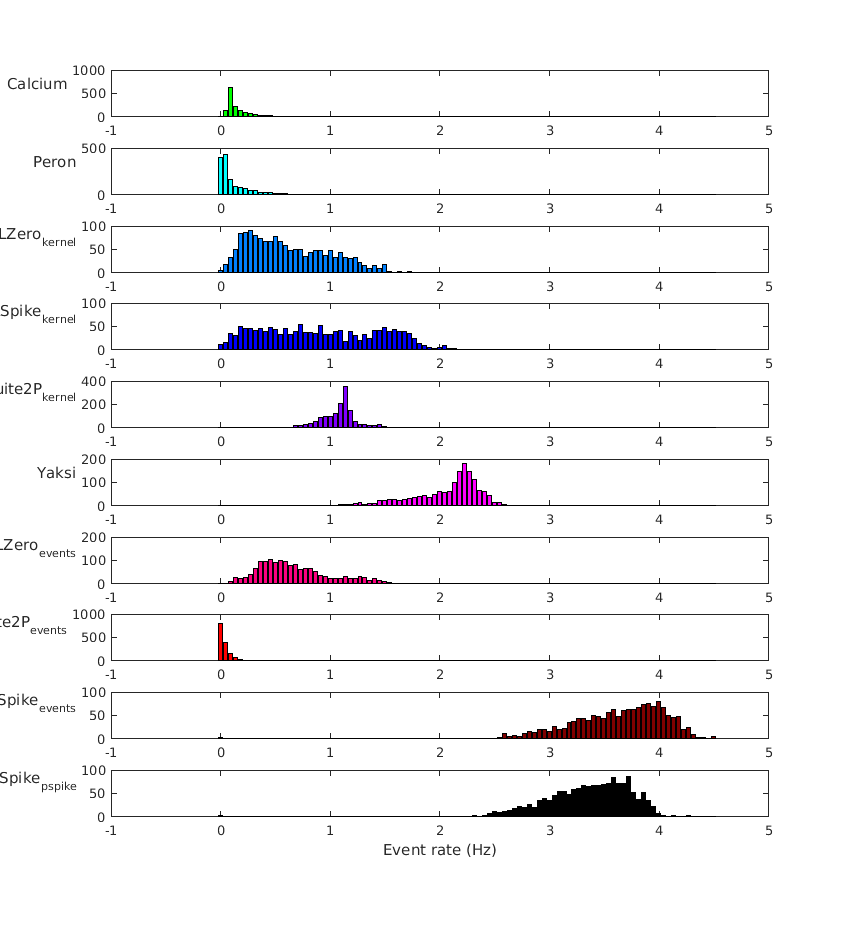
\includegraphics[trim={0 20 50 25},clip,width=0.5\textwidth]{figs/event_rate_all.png}}
\subfigure[]{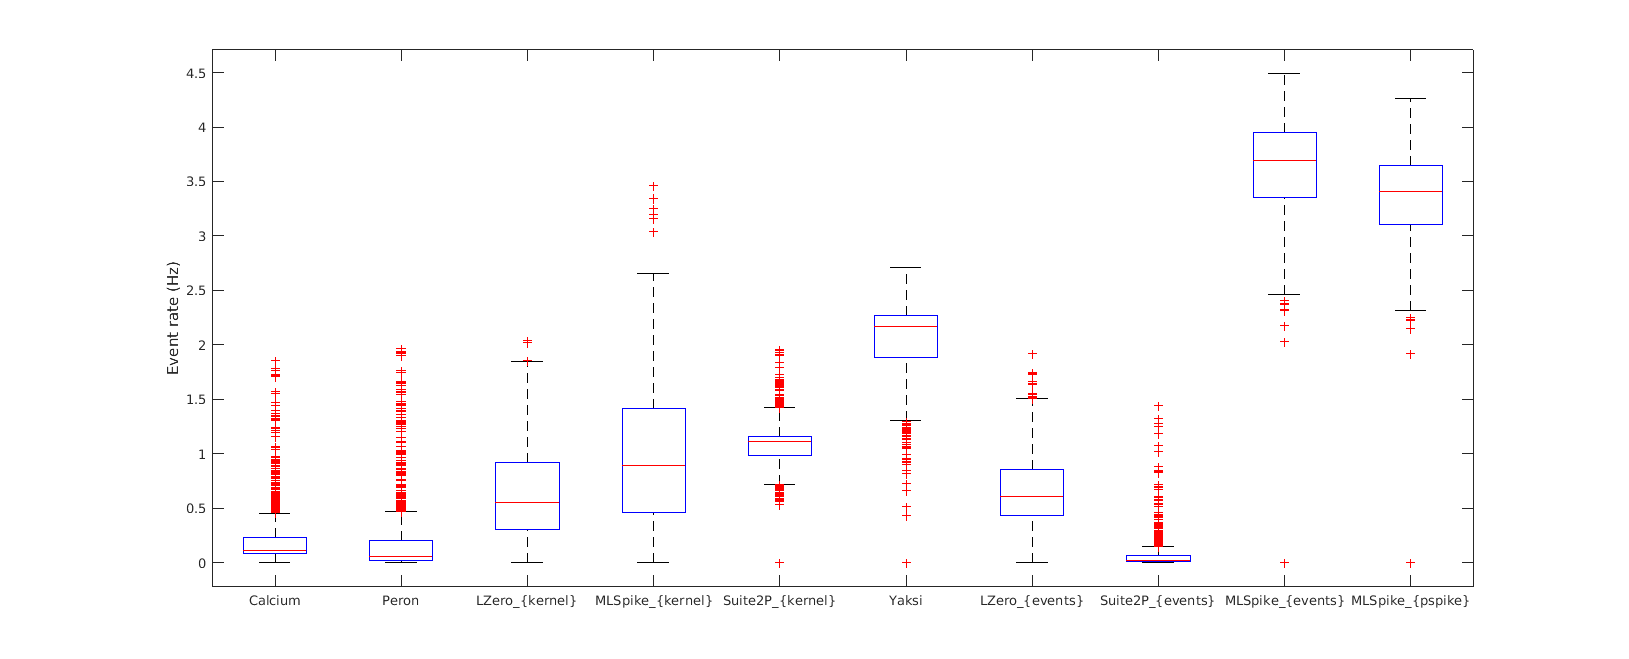
\includegraphics[trim={100 20 110 25},clip,width=0.5\textwidth]{figs/event_rate_dist_all.png}}
\subfigure[]{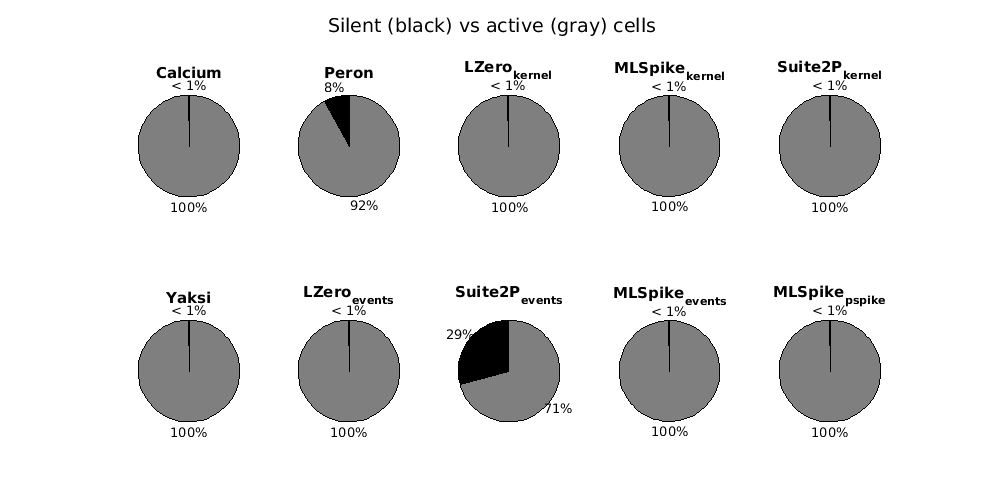
\includegraphics[trim={80 30 60 10},clip,width=0.5\textwidth]{figs/silent_cells_all.png}}
\caption{\label{fig:event_detection} Estimated 'event rate' for all cells in an example session. For the first 6 methods (Calcium - Yaksi), events are detected as fluorescence transients greater in magnitude than 3 std deviations of background noise. Background noise = data - smoothed version of data, to eliminate slow transients. Methods 7-10 (LZero$_{events}$ - MLSpike$_{pspike}$) return a spike count per time bin. (a) Boxplots of event rate per cell for each method. (b) Same data as in (a) but plotted as box and whisker plots. (c) Proportion of active (gray) vs silent (black) cells for each method. Silent = event rate < 0.0083Hz.}
\end{figure}

\clearpage
\subsection{Different spike inference methods lead to different estimates of task related neurons}

For many analyses, it is the relative activity of a cell and not it's exact firing rate that is important. A common analysis is to ask whether a neuron's activity is task related - does a cell respond more during a specific epoch of the task than would be expected from a random process. We quantified the proportion of task related neurons in our dataset following the approach of Peron et al 2015. Calcium/instantaneous firing rate/ events for each cell is shuffled in time before a trial-averaged PSTH is generated, and the largest peak in the PSTH is recorded. This is repeated 10,000 times. A distribution of PSTH peak magnitudes is generated, and if the peak of the true (data) PSTH is larger than the 95\%ile of the shuffled distribution, in either the Left or Right (Go, No Go) trials, that cell is considered 'tuned'.

Firstly, each method estimates a different proportion of tuned vs untuned cells, both in comparison to estimates from the raw Ca\textsuperscript{2+}, and in comparison to one another. Secondly, the methods only agree on the tuned status of individual neurons for $\sim$50 cells (from a range of 50 - 250 tuned cells). 

\textbf{TO DO: compute PSTH for tuned vs untuned cells. This may be the time to look at Yaksi $\&$ Friedrich style temporal correlations...}

\begin{figure}
\centering
\subfigure[]{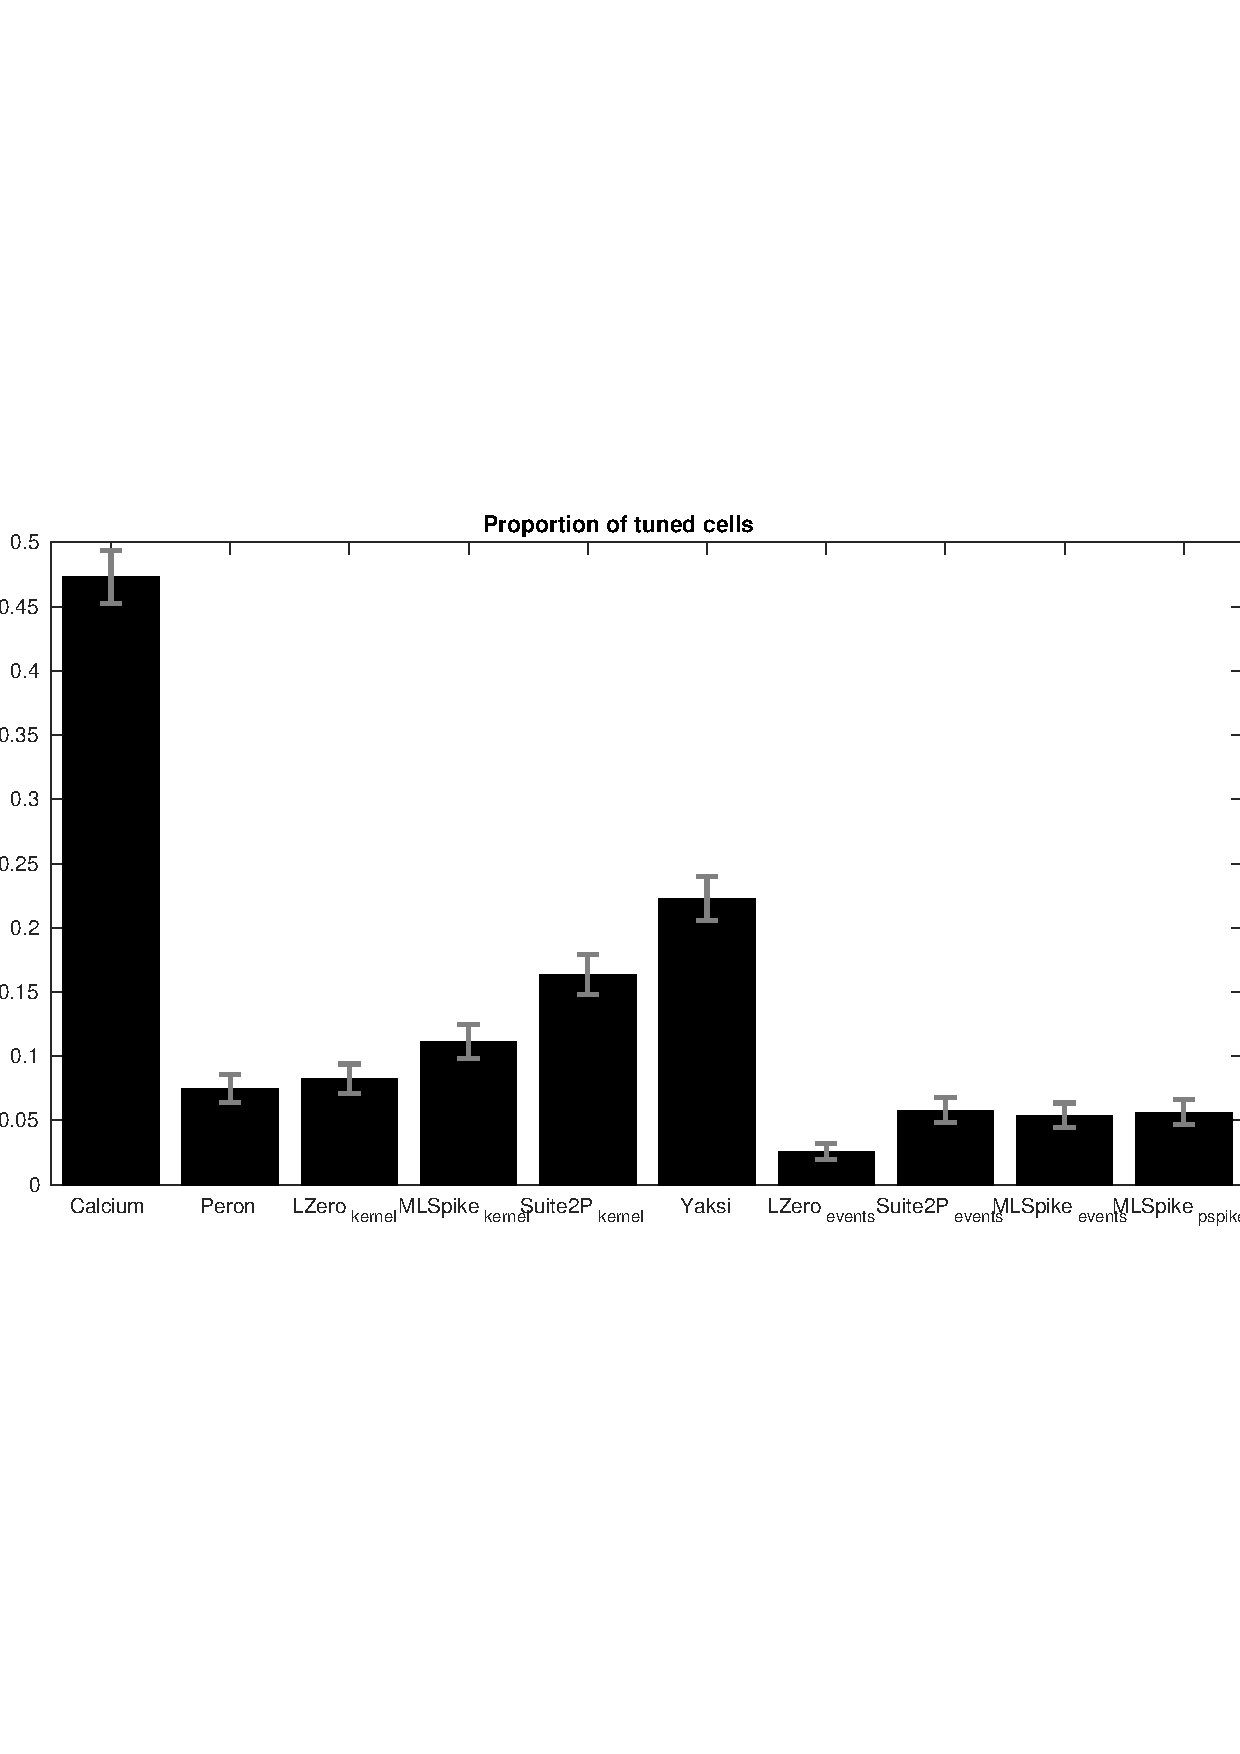
\includegraphics[trim={0 250 0 240},clip,width=0.7\textwidth]{figs/Tuned_cell_all_zoom.pdf}}
\subfigure[]{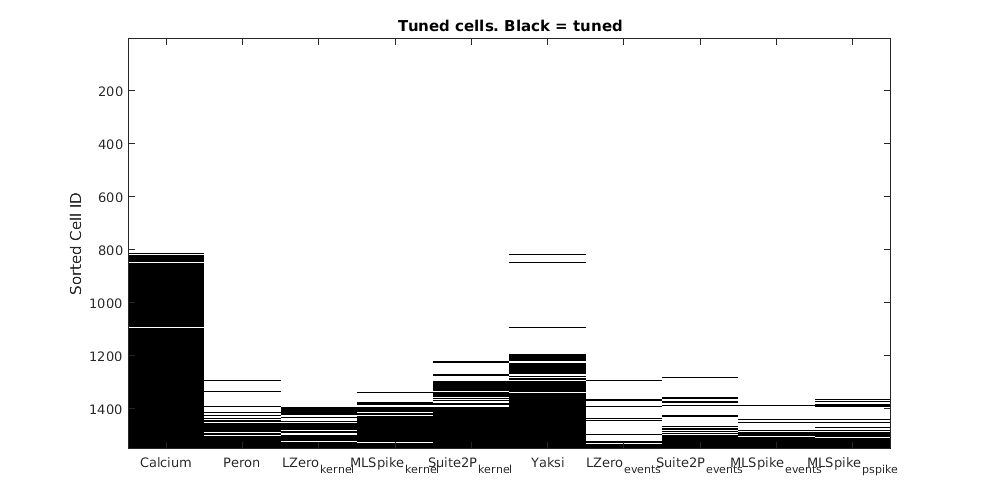
\includegraphics[trim={50 25 60 10},clip,width=0.7\textwidth]{figs/tuned_array2.png}}
\subfigure[]{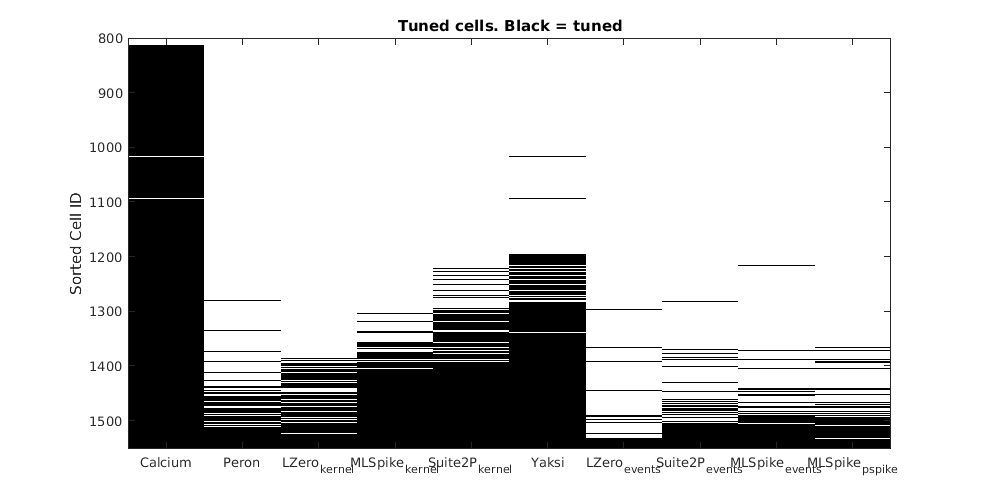
\includegraphics[trim={50 25 60 10},clip,width=0.7\textwidth]{figs/tuned_array2_zoom.png}}
\caption{\label{fig:tuned_cells} Tuned cells. Tuned cells were determined through shuffle tests (see main text).  (a) Number of tuned cells per deconvolution method. Error bars are 95\% binomial confidence intervals (Jeffreys interval) (b) Array of tuned cell identities. Black = tuned, white = not tuned. Rows are cells, ordered by the number of methods that classify that cell as tuned. (c) Zoomed in version of (b). There is substantial disagreement between methods.}
\end{figure}




%\begin{figure}[h!]
%\centering
%\includegraphics[width=1\textwidth]{VP96_D16.pdf}
%\caption{\label{fig:VP96}Spike metrics. Left: Victor and Purpura (1996) proposed a spike metric to compare spike trains. This metric is generated by determining the number of elementary operations (shift, addition, or deletion of individual spikes) required to match two spike trains, up to some temporal precision (here 0.5s). Right: In Deneaux et al 2016 the Error Rate (ER) is similarly computed as a ratio of sensitivity vs precision in spike detection. Detections are counted to within 0.5s.}
%\end{figure}



% \begin{figure}[h!]
% \centering
% 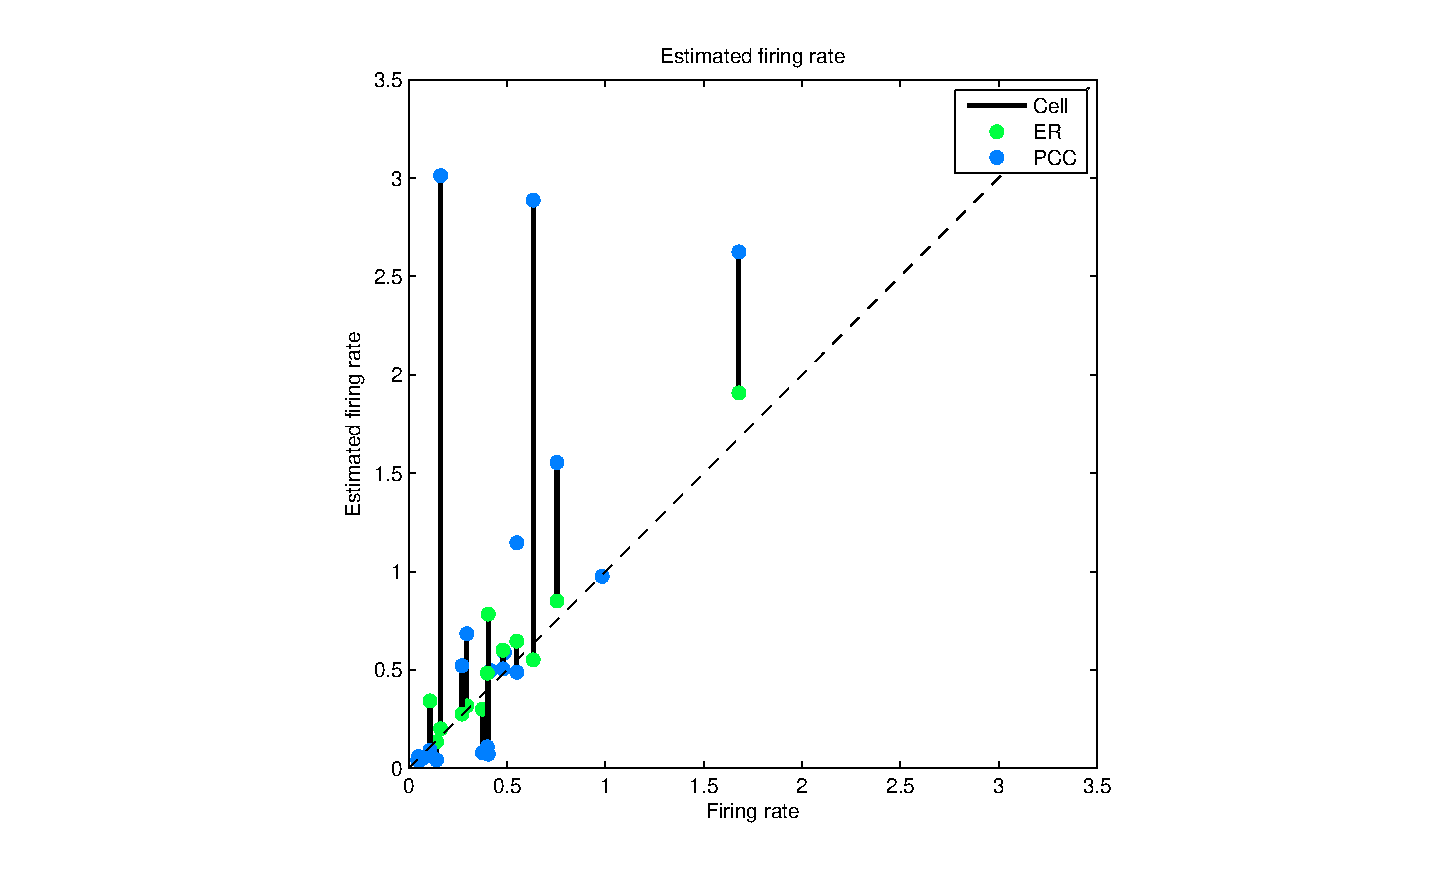
\includegraphics[width=1\textwidth]{ER_PCC_FR_compare.eps}
% \caption{\label{fig:deconv_FR} PCC overestimates firing rate}
% \end{figure}



\newpage

\subsection{Deconvolution leads to biased and noisy estimates of pairwise correlation}
\emph{Deconvolution is always a trade-off between false positives and misses, meaning you get both\\
Miss real spikes + overestimate background rates (see also Ganmor), therefore\\
\indent - correlation estimates are noisier (due to false positives) or biased (due to misses/decorrelation)\\
\indent - TO DO: add in 4 new methods. Also sparse noise for the noise example?\\
\indent  - TO DO: add variance explained by eig decomposition plot\\
%\indent - TO DO (?) repeat this analysis but with deconvolved events where available
\indent - MLSpike and Suite2P - using parameters tuned to increase ER on ground truth data - have broader distributions more similar to that resulting from smoothing the raw Ca\textsuperscript{2+}. The Peron events have a large number of PCCs below zero, suggesting that choosing parameters that penalise false-positives may be actively decorrelating the data. }

A goal of many Ca\textsuperscript{2+} imaging experiments is to record from populations of neurons, and then perform clustering or dimensionality reduction. These analyses rely on estimates of pairwise correlations. Figure \ref{fig:PCCs} (a) and (c) show the distributions of pairwise correlation coefficients computed separately for each method. To aid interpretation of these results we also computed pairwise correlations for five different data surrogates: \\
\indent - Shifted: the fluorescence time series for each cell was randomly shifted in time (using Matlab's circshift function) by up to 10000 frames. \\
\indent - Scrambled - elements of the original N x T data matrix were sampled randomly (without replacement) to generate a new data matrix. \\
\indent - Randn - pseudorandom values drawn from a normal distribution. \\
\indent - Conv (kernel) - original data convolved with an exponentially decaying kernel as is used in the MLSpike and Suite2P deconvolution methods. \\
\indent - Shuffled rows - like the 'scrambled' data, but shuffling was done separately for each cell (rows of the data matrix) to preserve differences in event rate across neurons \emph{NB this shouldn't be any different to the scrambled data as PCC is invariant to affine transformations i.e. same tuning but larger changes in firing rate....}\\

MLSpike and Suite2P - using parameters tuned to increase ER on ground truth data - have broader distributions more similar to that resulting from smoothing the raw Ca\textsuperscript{2+}. The Peron events have a large number of PCCs below zero, suggesting that choosing parameters that penalise false-positives is actively decorrellating the data. 




%\subsubsection*{Correlations}
% IDEA: Compute PCCs with decorrelated events computed with different parameters. How does the distribution move?

%[trim={50 10 50 10 },clip,width=0.8\textwidth]{pairwise_scatter2.eps}}
%[trim={50 10 50 10 },clip,width=0.8\textwidth]{pairwise_kernel2.eps}}

\begin{figure}[h!]
\centering
\subfigure[]{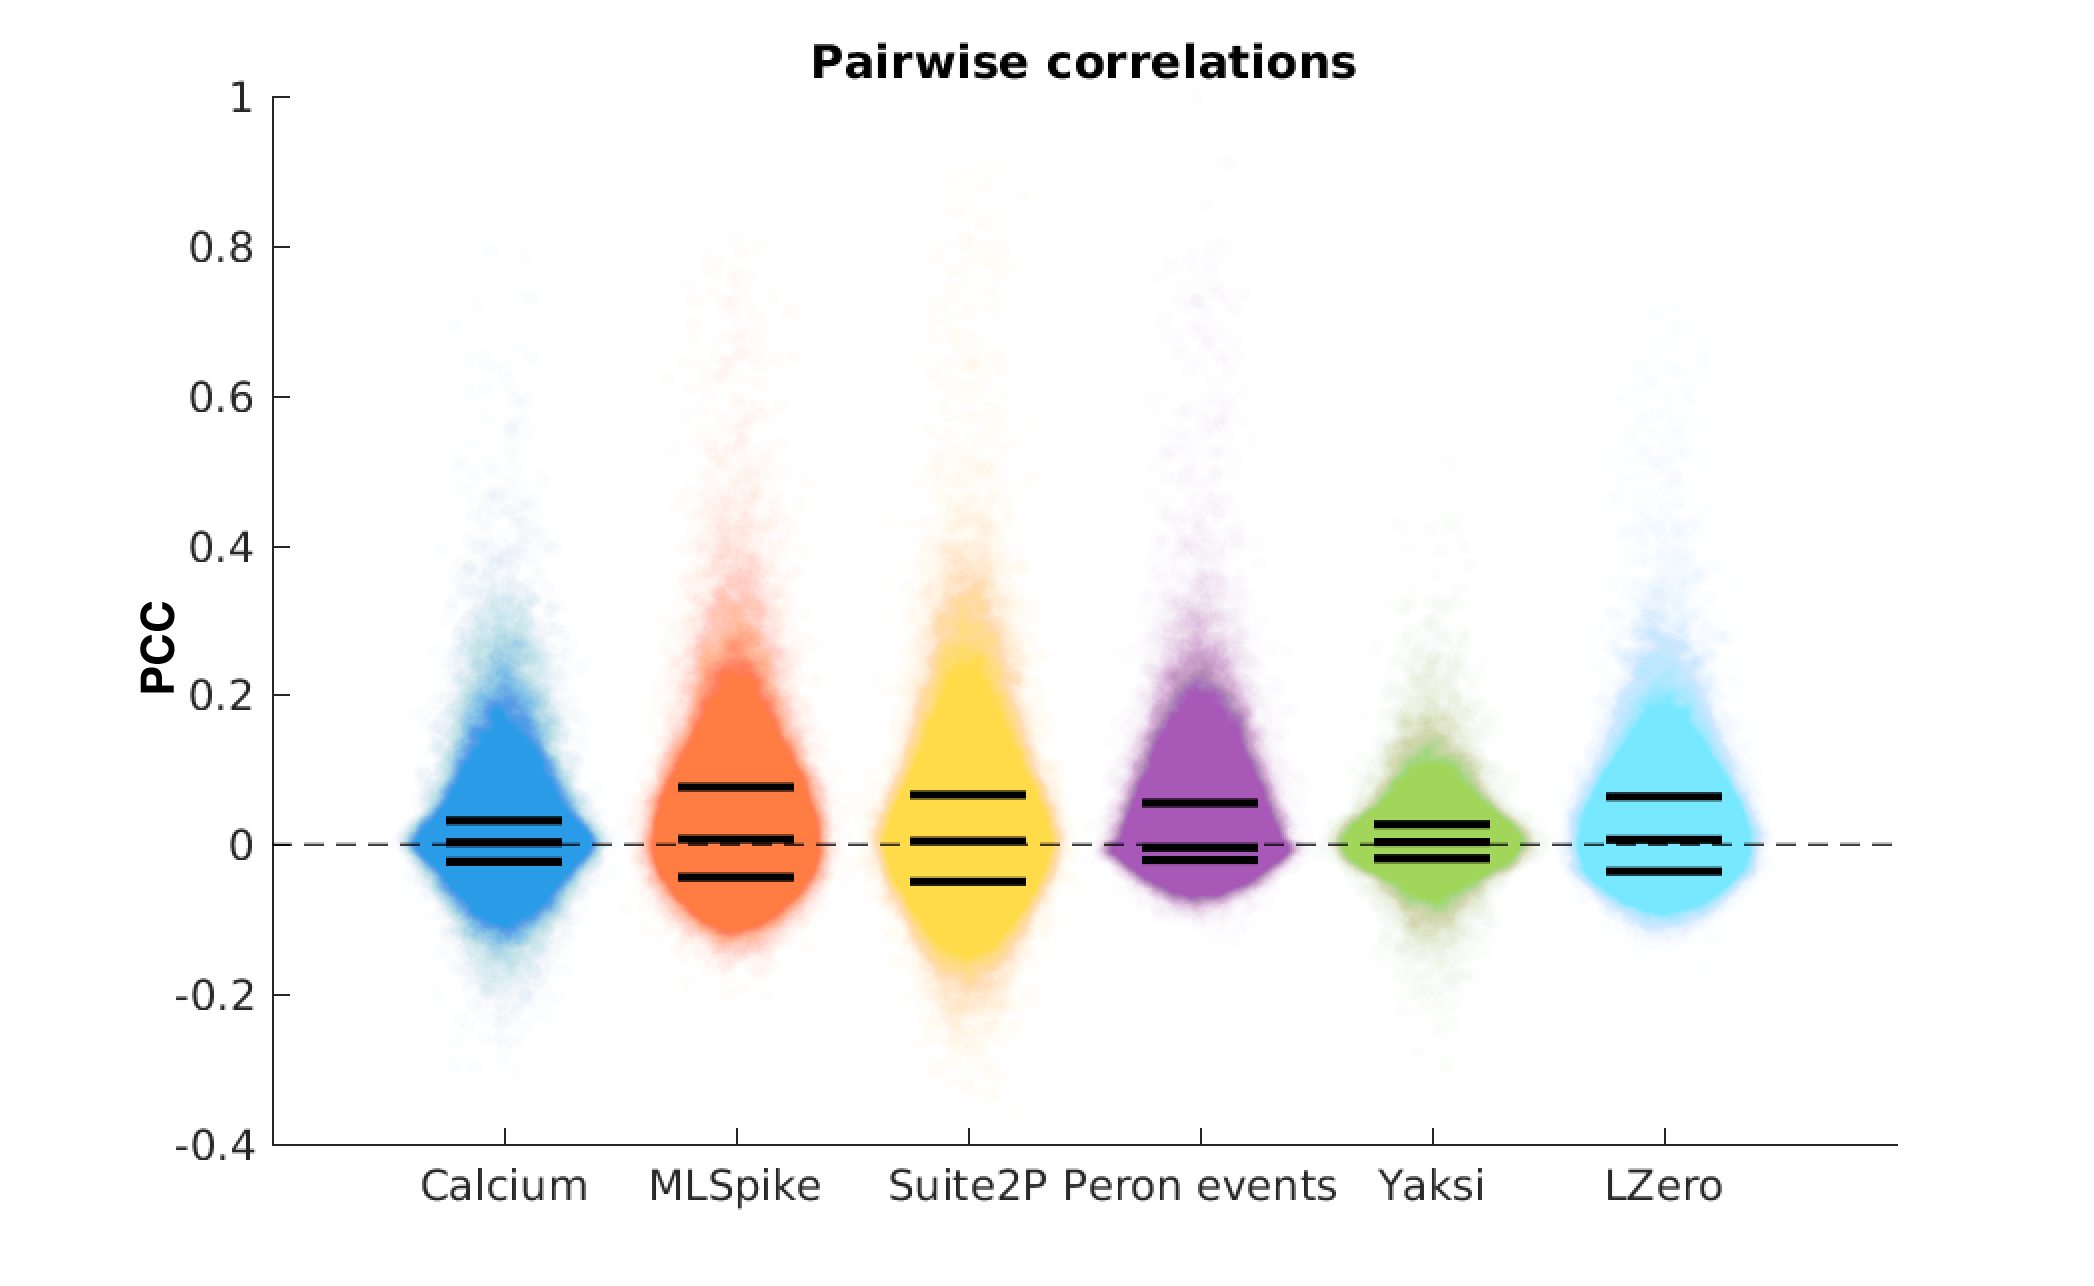
\includegraphics[trim={10 10 10 10 },clip,width=0.45\textwidth]{figs/pairwise_scatter3_alph_pt01.png}}%
\subfigure[]{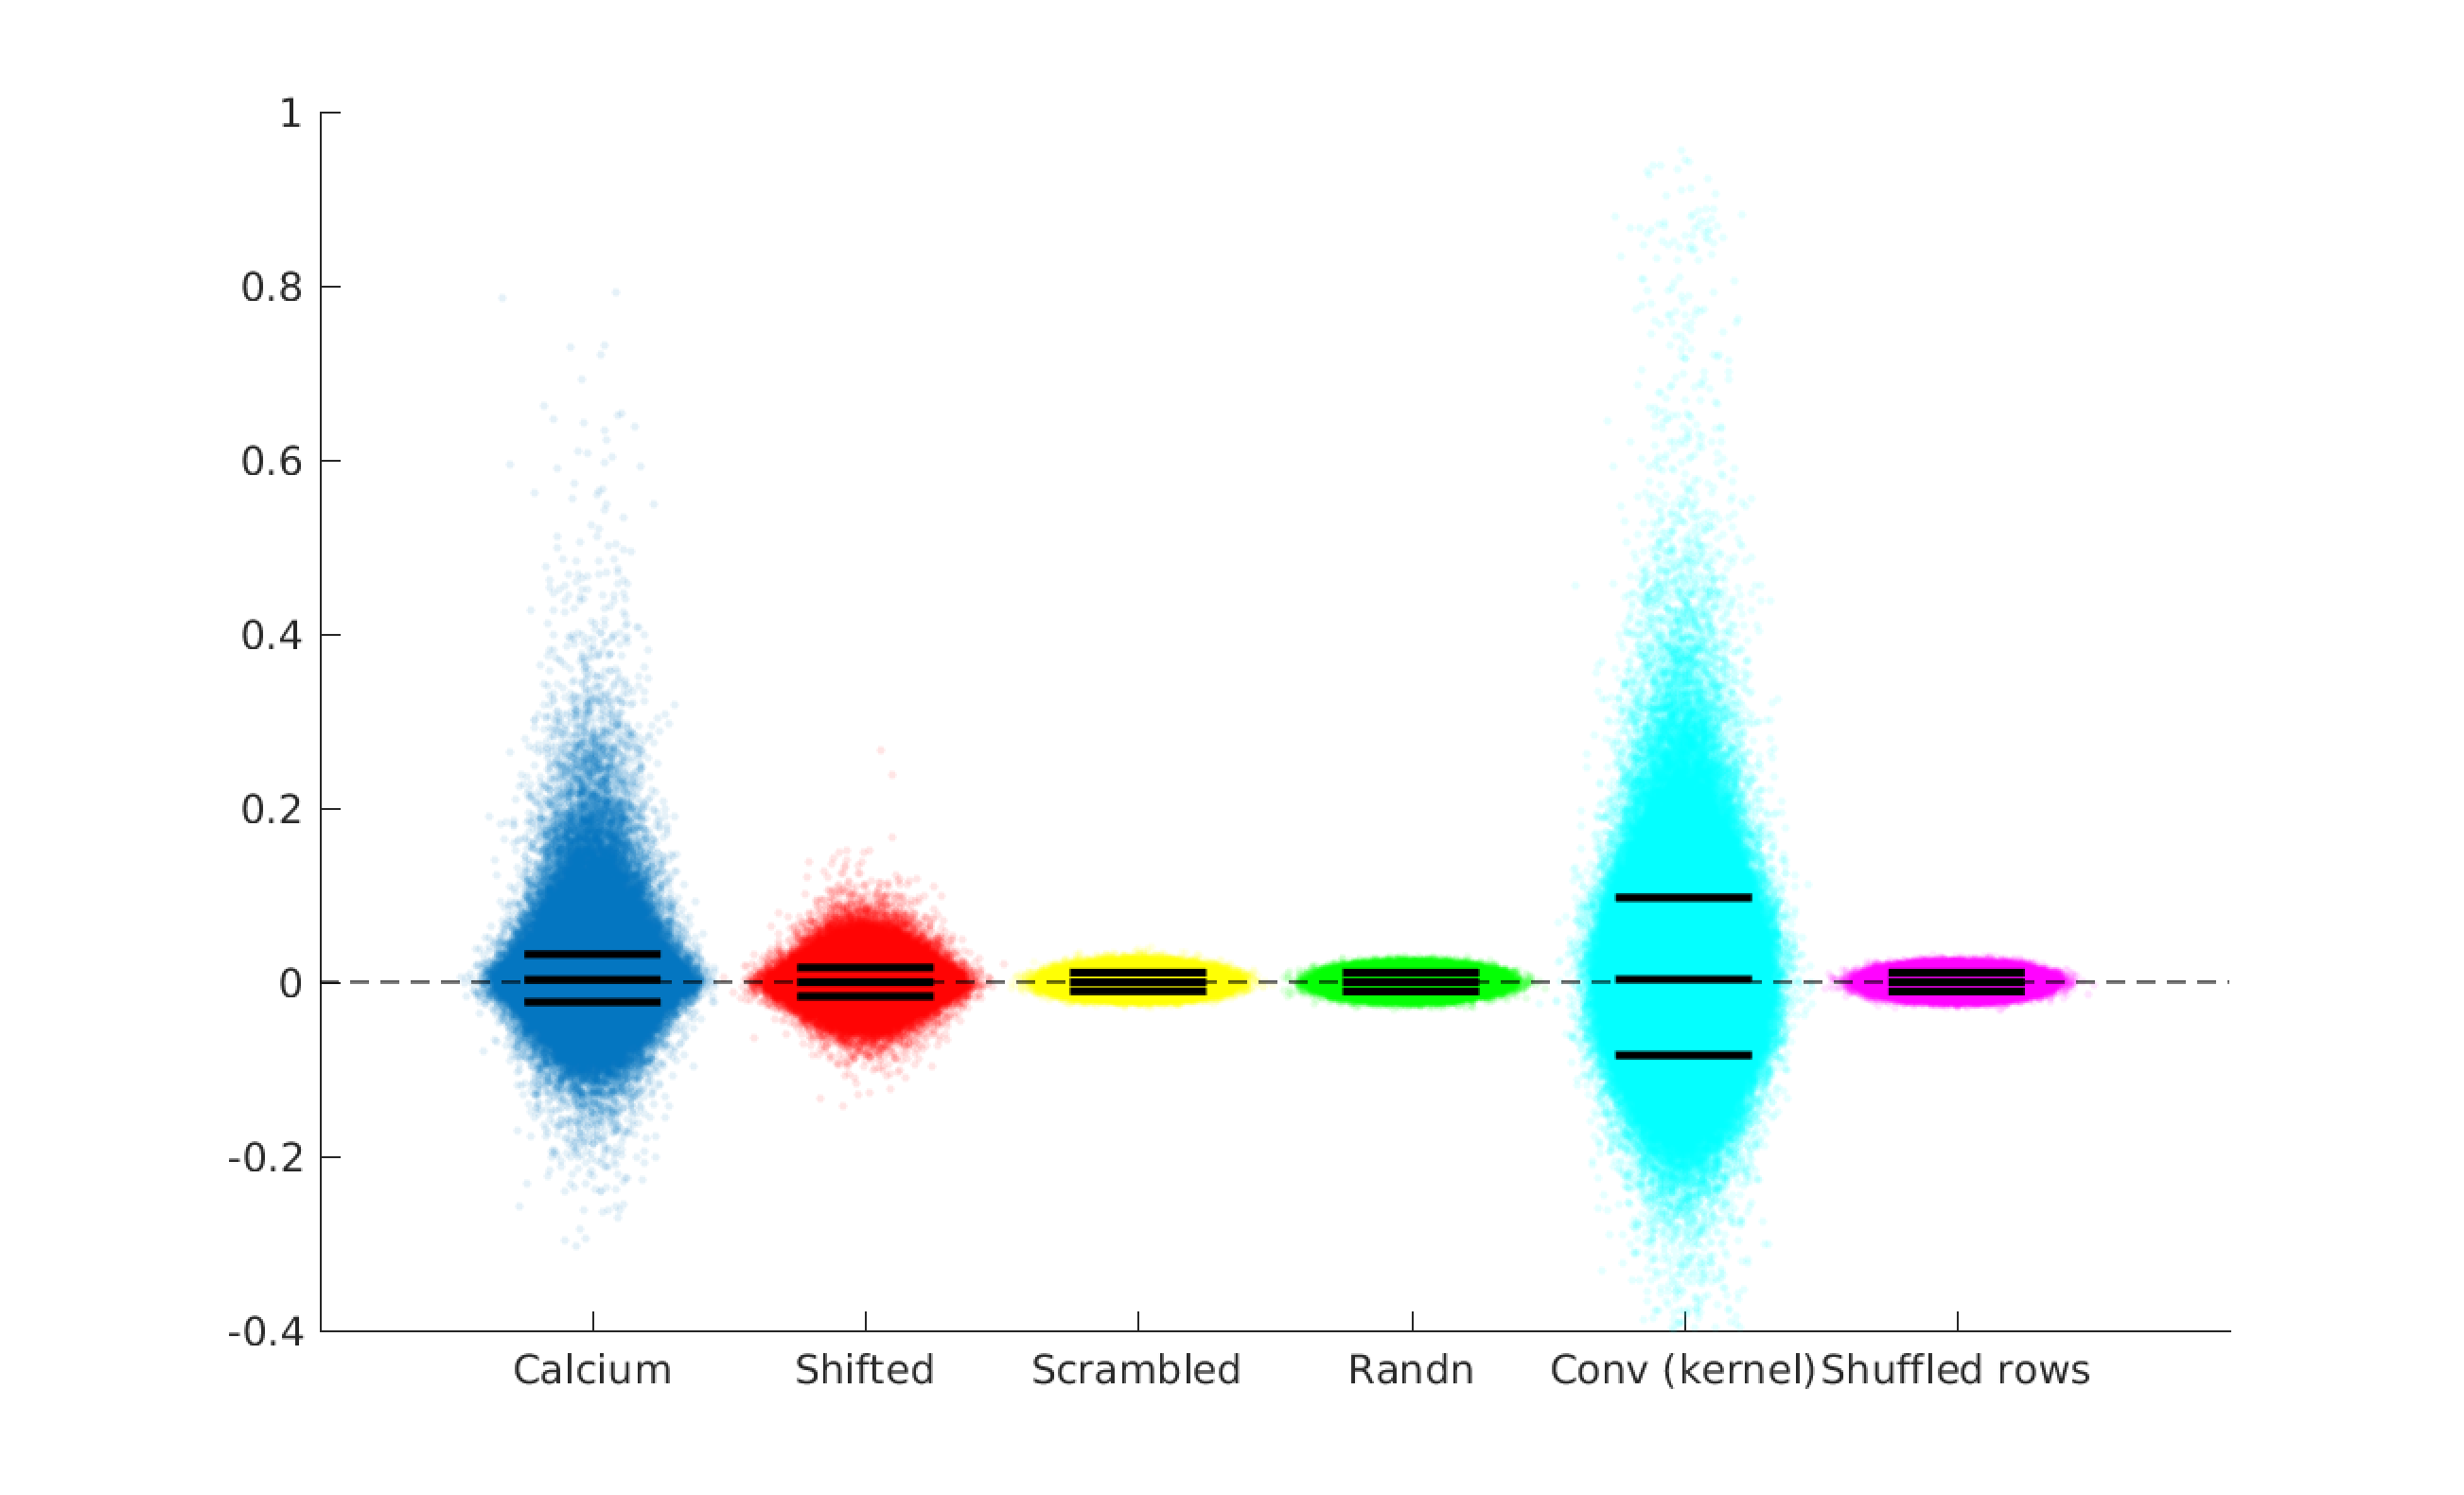
\includegraphics[trim={10 10 10 10 },clip,width=0.45\textwidth]{figs/noise_comparison3CI.png}}
\subfigure[]{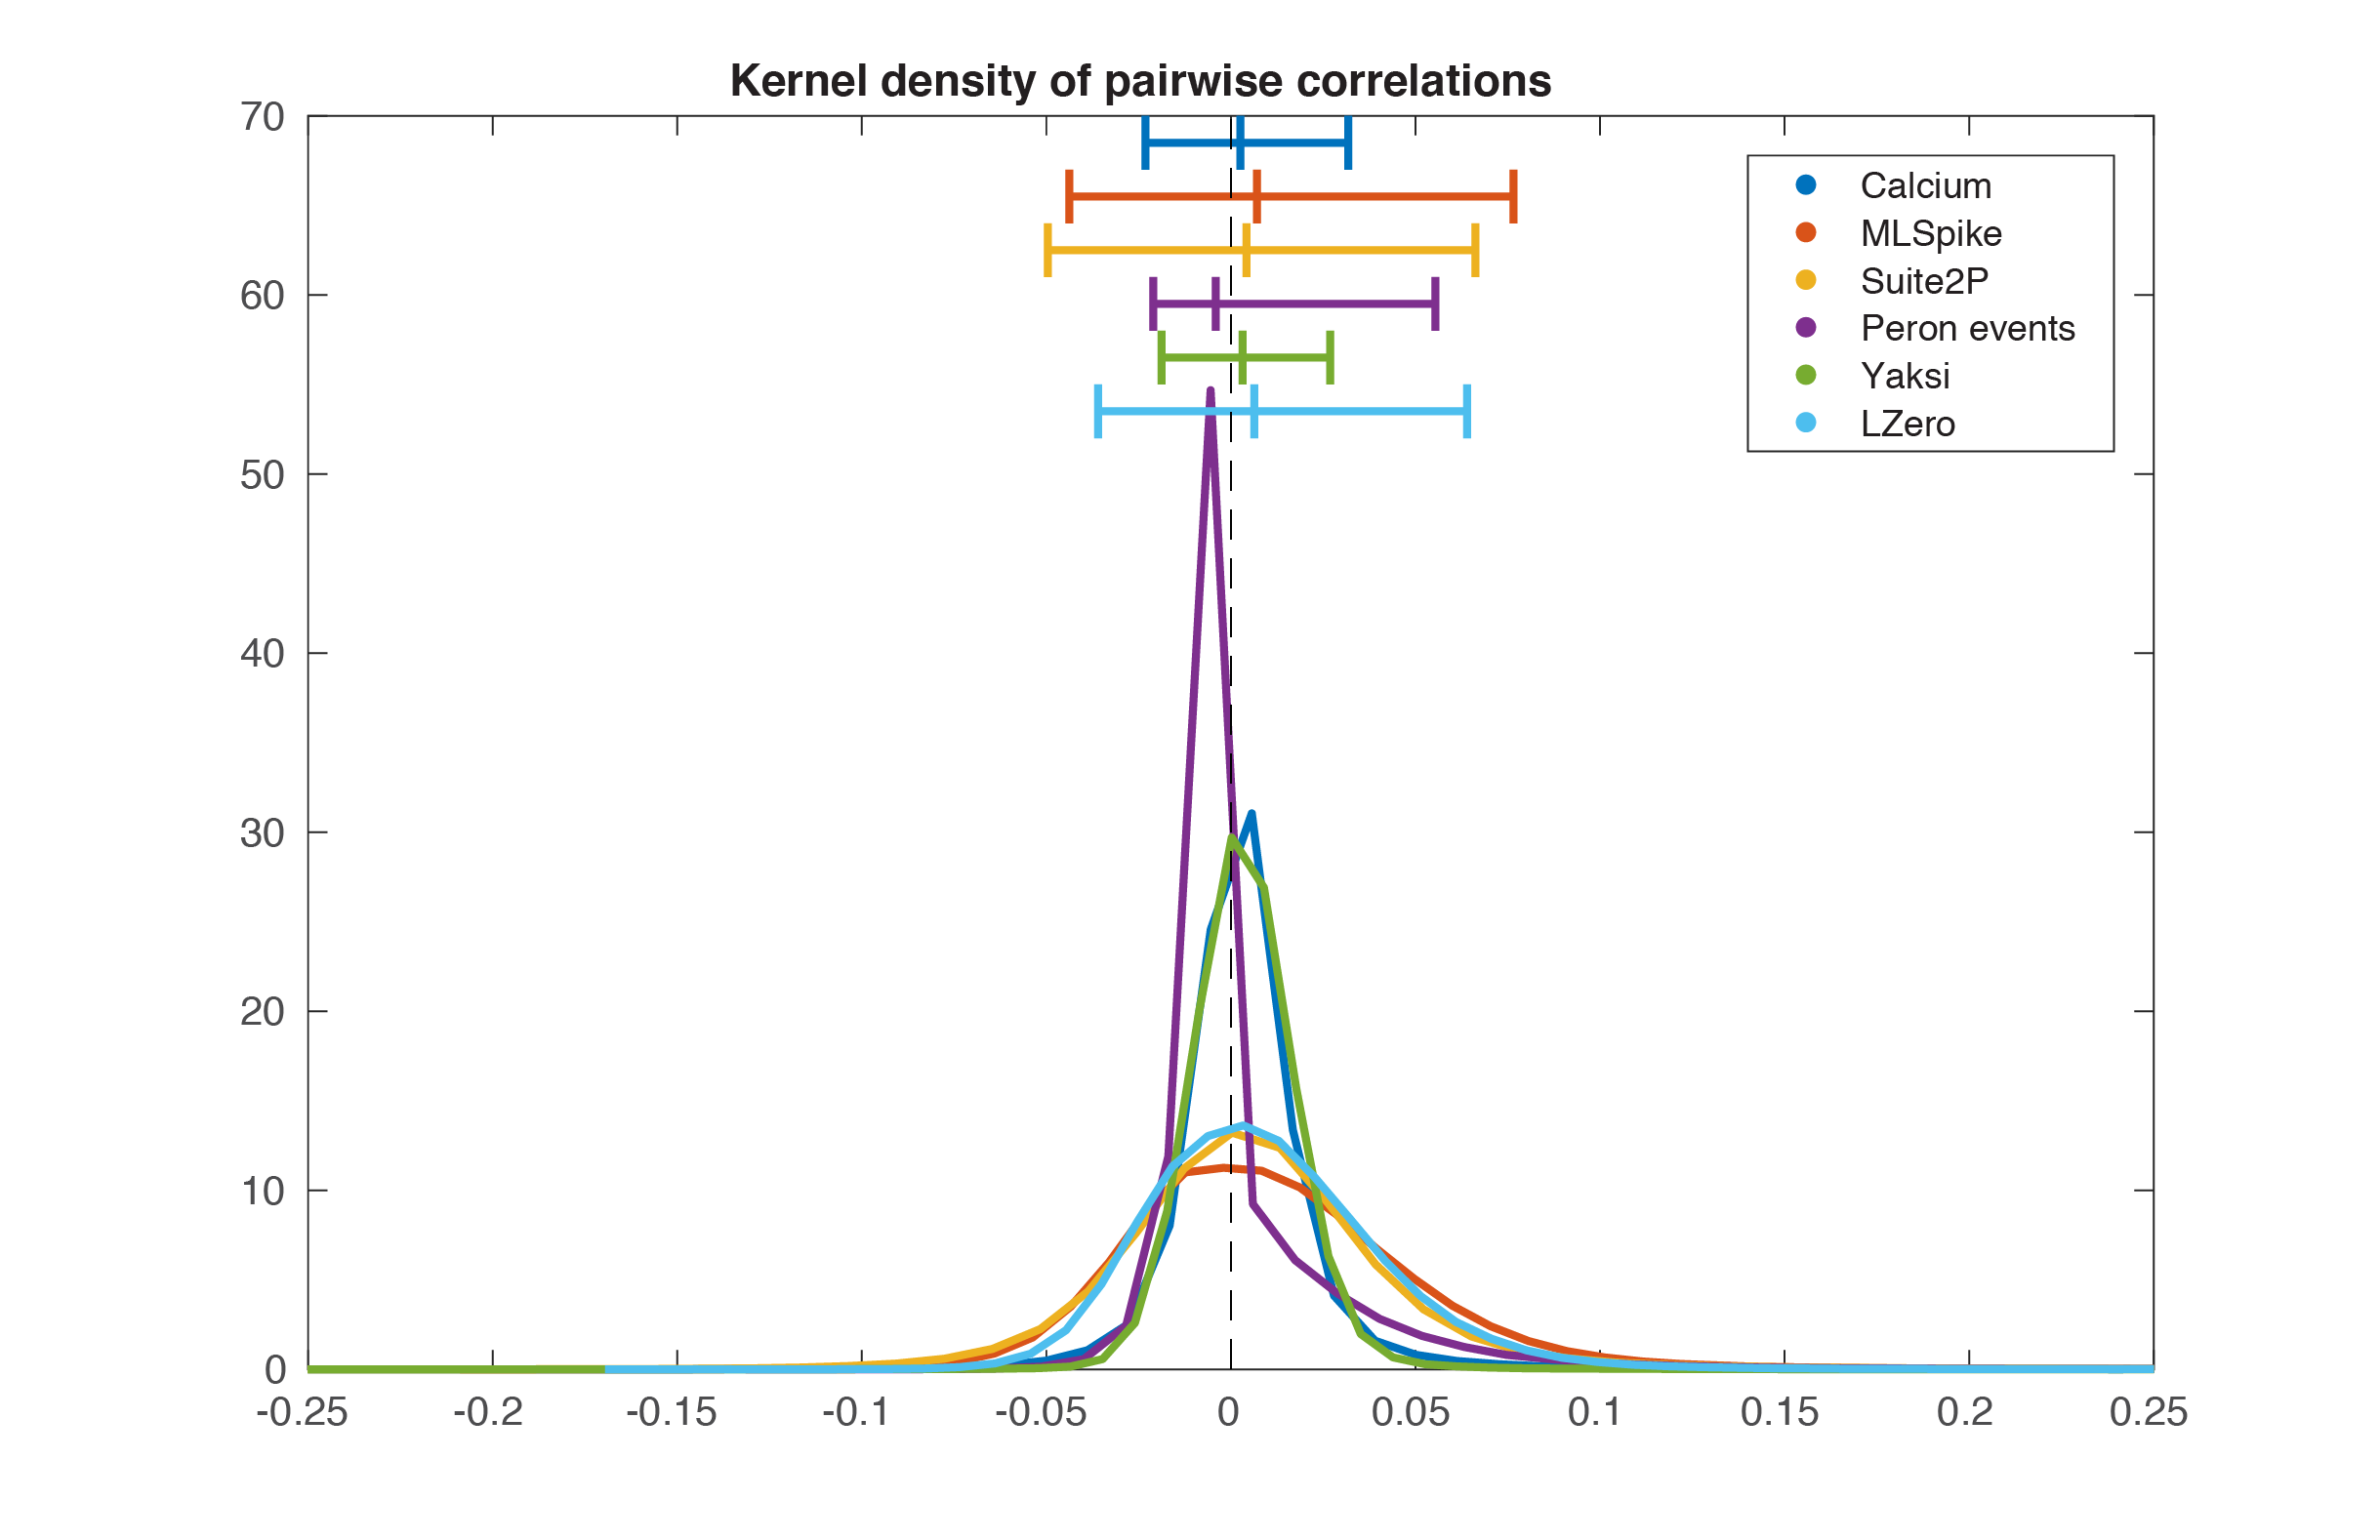
\includegraphics[trim={10 10 10 10 },clip,width=0.45\textwidth]{figs/pairwise_kernel3CI.png}}%
\subfigure[]{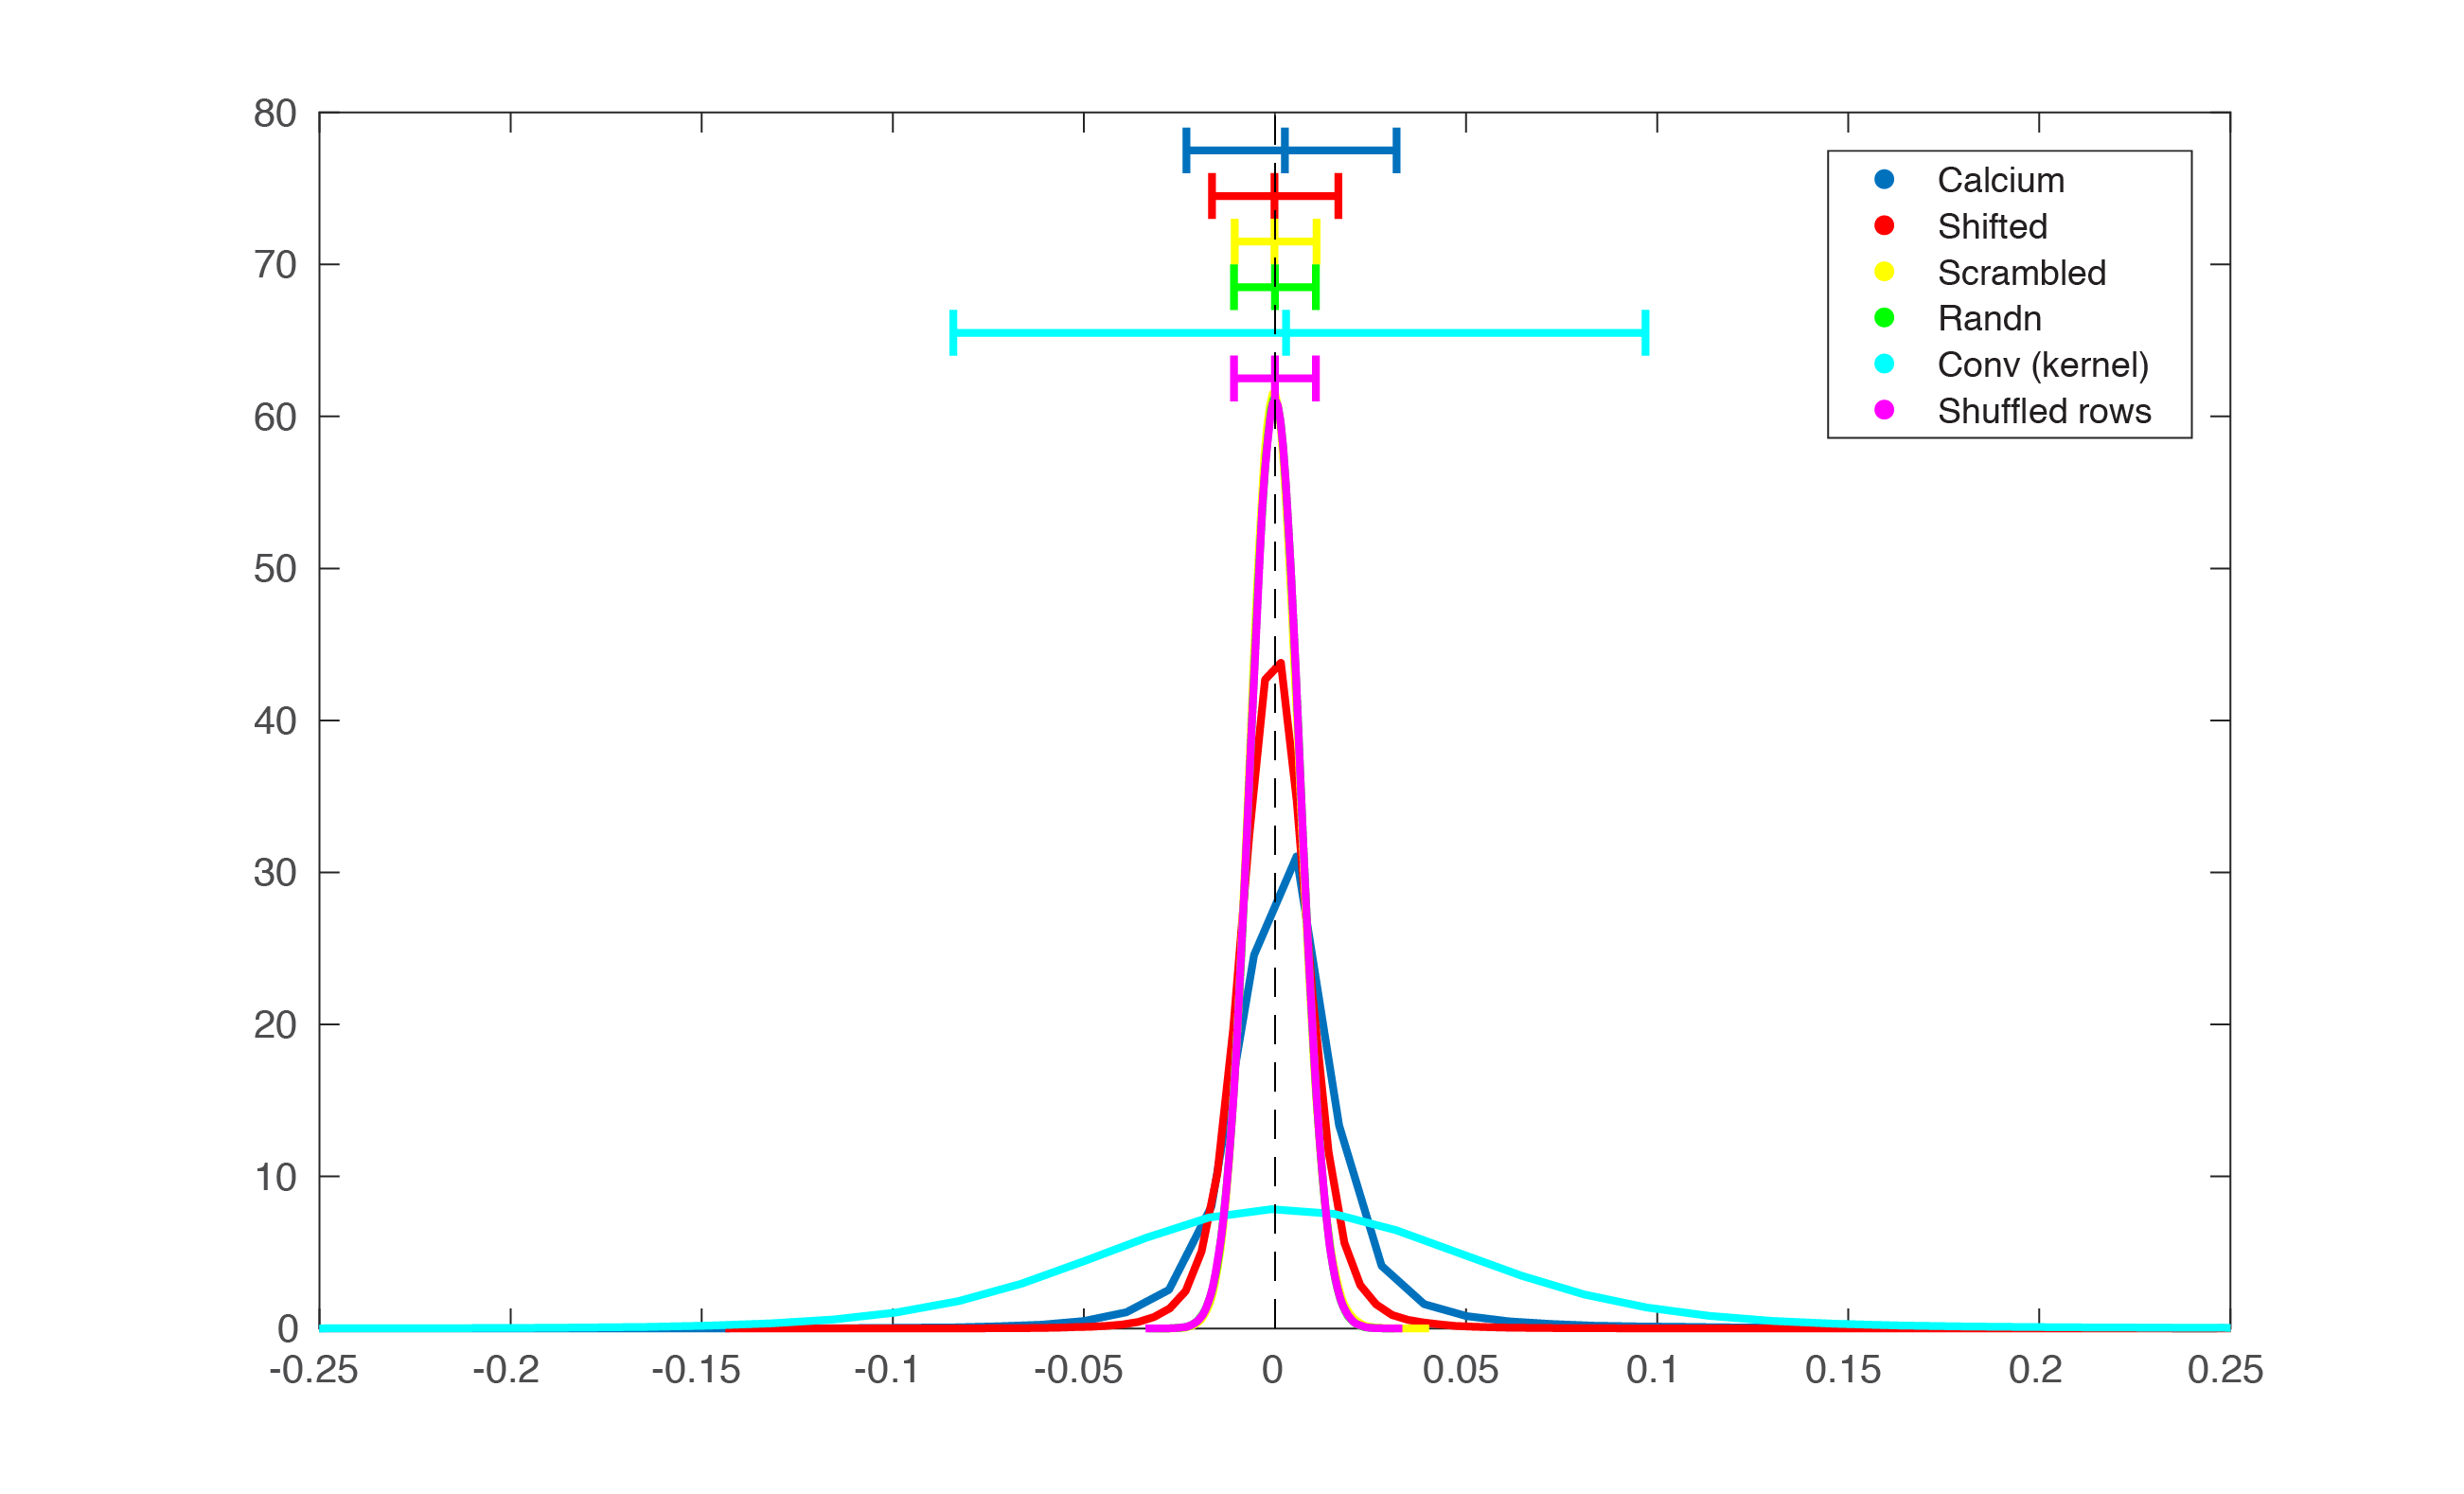
\includegraphics[trim={10 10 10 10 },clip,width=0.45\textwidth]{figs/noise_comparison3_kernel.png}}

\caption{\label{fig:PCCs} Pairwise correlations. (a) For each method (colours) each dot is the Pearson correlation coefficient between each pair of neurons (1203576 unique pairs, excluding self-correlations). X-axis jitter added for clarity. Black lines correspond to 5th, 50th (median) and 95th percentiles of the data. (c) Kernel density plots of data in (a). Lines above density plots correspond to 5th, 50th (median) and 95th percentiles of the data, coloured to match the distributions. (b) and (d) are the same as (a) and (c) but with different permutations or surrogates of the data. Calcium - data as in (a). See main text for details.}
\end{figure}


\begin{figure}[h!]
\centering
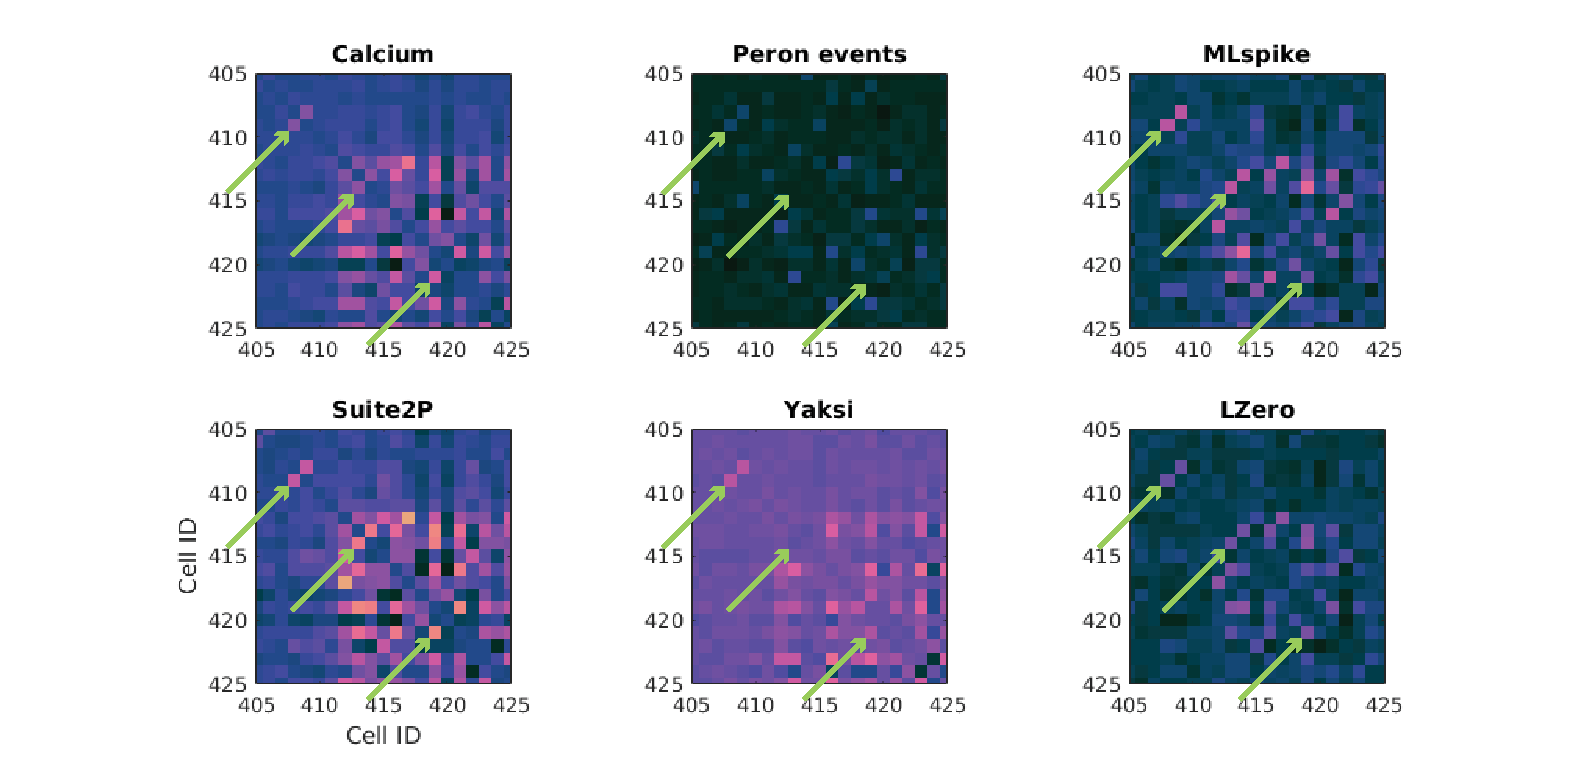
\includegraphics[trim={50 10 50 10},clip,width=0.8\textwidth]{pcc_all_image2_zoom.eps}
\caption{\label{fig:PCC_example} Peron events and Yaksi may actively decorrelate neurons. Each panel shows a subset of pairwise correlations between neurons from one session of data from Peron et al 2015, one panel for each method. Some pairs (arrows) showing high correlation across methods are missing (middle arrow) for the Peron events and Yaksi methods.}
\end{figure}

%\subsubsection*{Tuning}

\clearpage
\subsection*{Deconvolution does not improve the precision of temporal resolution under realistic conditions}
\emph{Comparison of estimates when deconvolving vs not\\
\indent - signal to noise \\
\indent - temporal resolution (rise/decay time)\\
\indent - TO DO: Repeat this analysis with deconvolved events\\
\indent - TO DO: Temporal correlations. Pick small number of cells e.g. of touch tuned vs some other parameter, and compute their correlations over time. Yaksi and Friedrich showed an advantage in their hands. \\}

To determine whether deconvolution improves the temporal precision of analyses such as tuning curves we computed the touch-triggered average for all cells in the example dataset. In the somatosensory system, touch onset is a salient sensory signal known to drive a subset of neurons with short latency and low jitter (O'Connor et al 2010, Hires et al 2014). \emph{To be continued...}

\begin{figure}[h]
\centering
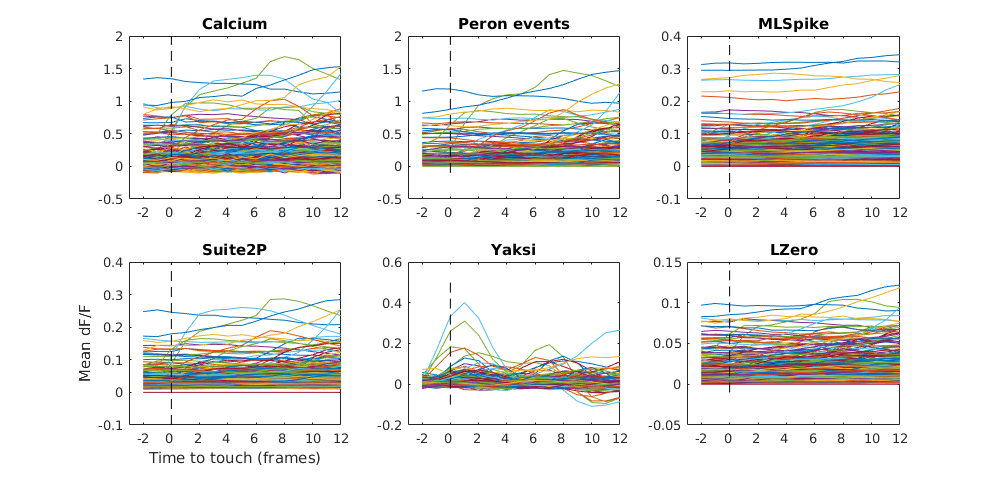
\includegraphics[width=1\textwidth]{tth_all.png}
\caption{\label{fig:tth_all} Comparing touch-triggered average (mean deconvolved FR per imaging frame) from different deconvolution methods for one all cells. Touch occurs at time zero. Only the Yaksi method shows a temporally sharp touch response.}
\end{figure}

\begin{figure}[h]
\centering
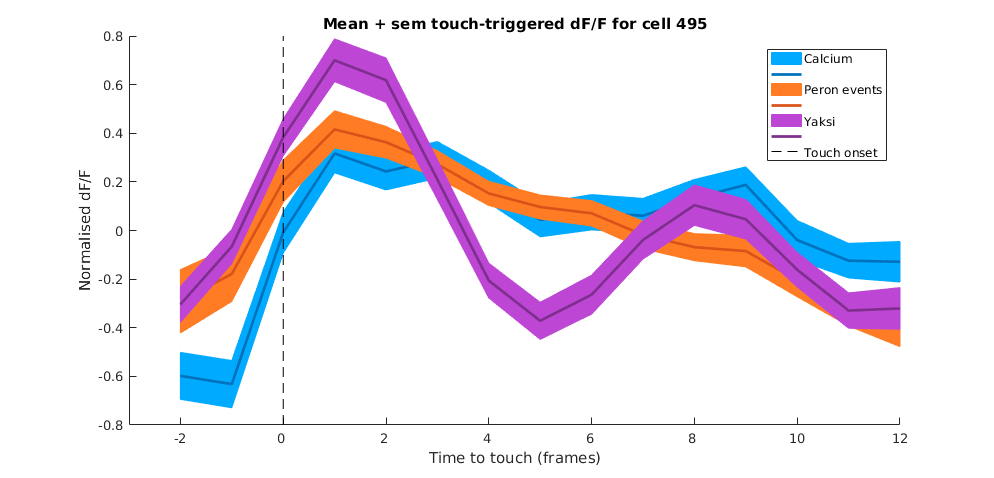
\includegraphics[width=1\textwidth]{tth_495.png}
\caption{\label{fig:tth_495}Comparing touch-triggered average (mean and s.e.m) from different deconvolution methods for one cell. Touch occurs at time zero. While the Yaksi method shows a temporally precise touch response, decaying within 1s (<7 frames), the Calcium and Peron events show a sustained response.}
\end{figure}

\begin{figure}[h]
\centering
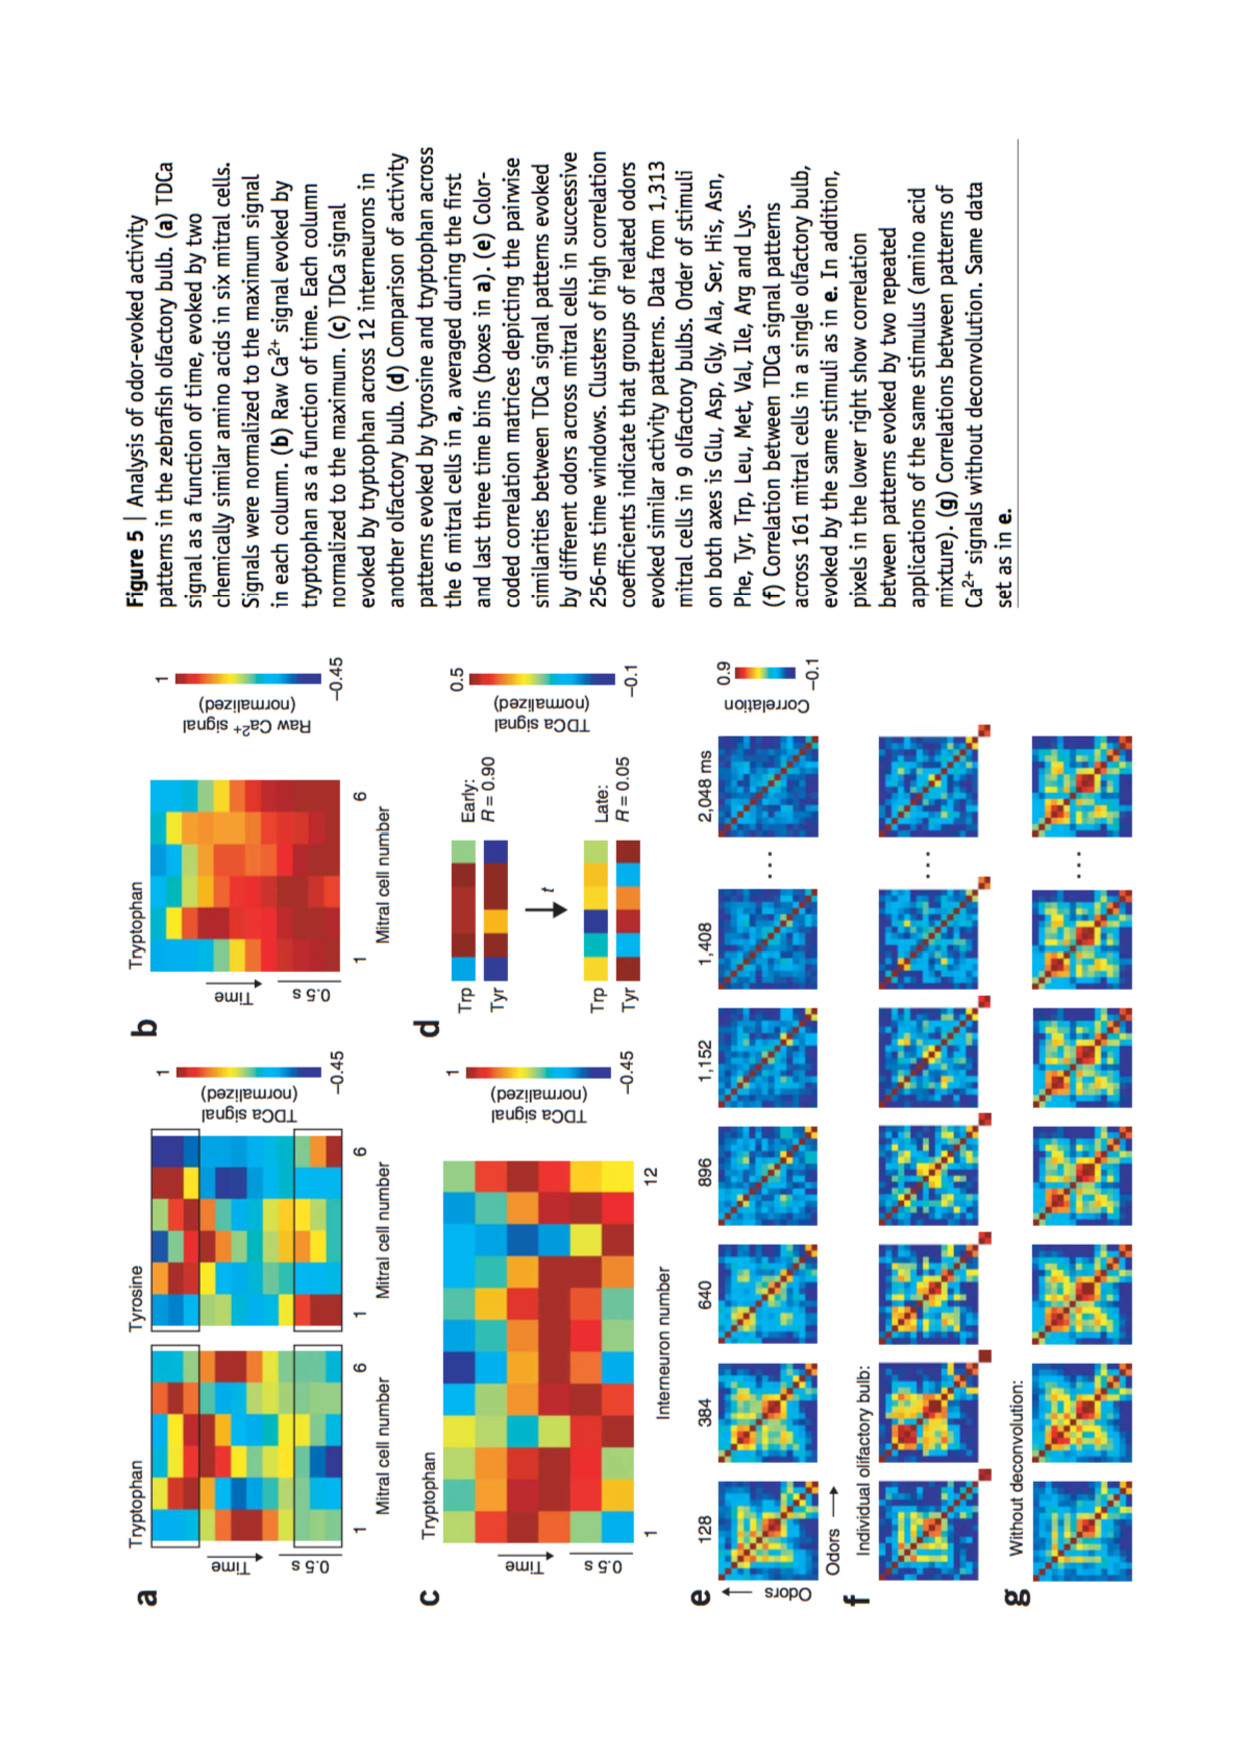
\includegraphics[height=\textwidth, angle = 270]{Yaksi_results2.pdf}
\caption{\label{fig:Yaksi_time} Deconvolution resolves the fine timescale of pairwise correlations, fig from Yaksi and Friedrich (2006). Perhaps a touch-triggered or 'persistent delay period activity' version of this would be interesting?}
\end{figure}

\clearpage
\subsection*{Spike inference does not automatically remove experimental artefacts}
Apart from improving estimates of neural activity, spike inference is also used to remove artefacts from the data such as slow drifts in fluorescence across experiments, or differences in single-spike fluorescence across cells. In head fixed imaging experiments, licking behaviours can lead to a dip in Ca\textsuperscript{2+} fluorescence (Simon Peron, personal communication). However, Figure \ref{fig:lick_PSTH} shows that this dip is also present in deconvolved traces (TO DO ADD FIG).

\begin{figure}[h!]
\centering
%\subfigure[]{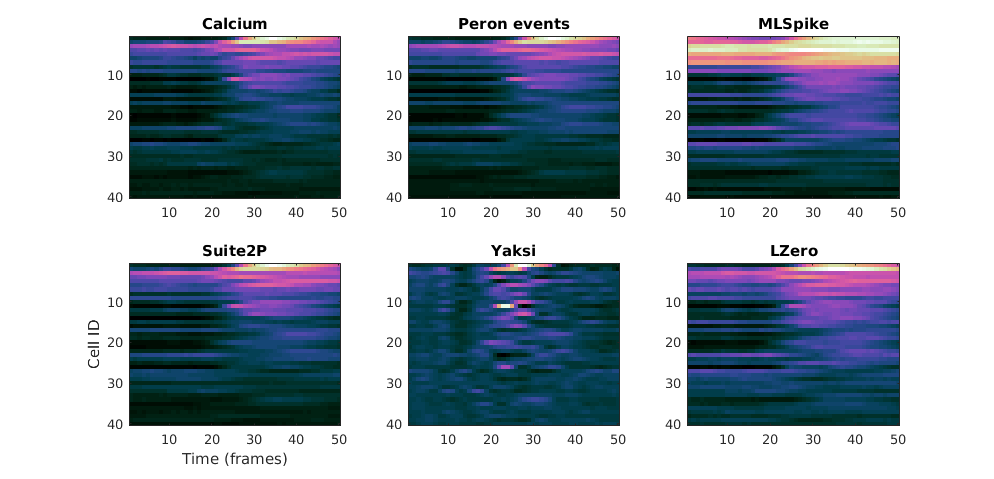
\includegraphics[width=0.9\textwidth]{psth2_40.png}}
%\subfigure[]{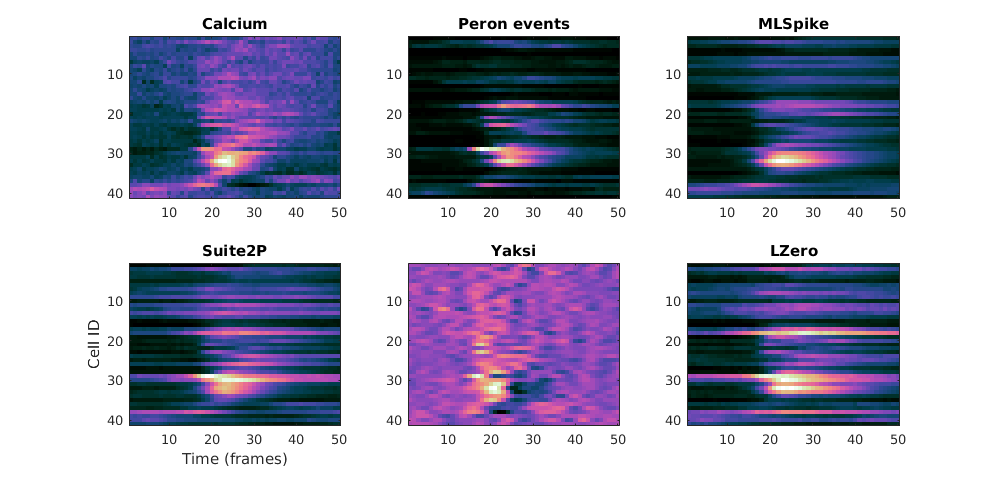
\includegraphics[width=0.9\textwidth]{psth2_720.png}}
\subfigure[]{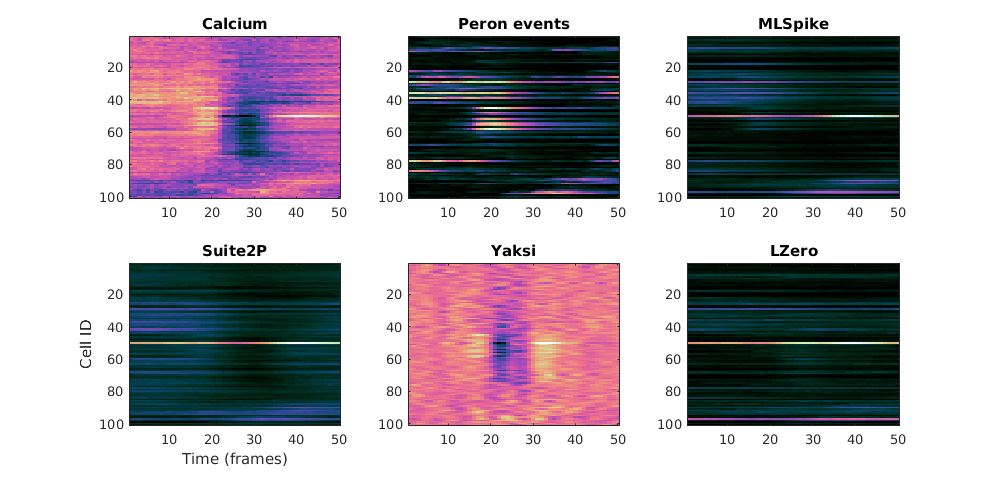
\includegraphics[width=0.9\textwidth]{psth2_1260.png}}
\caption{\label{fig:lick_PSTH} PLACEHOLDER FIGURE. Lick induced dip in Ca\textsuperscript{2+} fluorescence seen in the raw Calcium is also seen in deconvolved data.}
\end{figure}

%PSTHs do not show obvious increase in temporal sharpness following deconvolution, but do show signs of missing important features of the data. Each panel shows a different cluster of neurons sorted by t-SNE ordering of PSTHs derived from Calcium data. Pole up is at frame 9, pole down at frame 17, and reward cue is at frame 22. NOTE: Group 3 is aligned to the (likely lick artefact induced) dip in df/f. If this is indeed artifactual, the change in signal still results in a 'rebound' response using Peron (and others, when looking at raw data, figures not shown here)}

%\begin{figure}[h!]
%\centering
%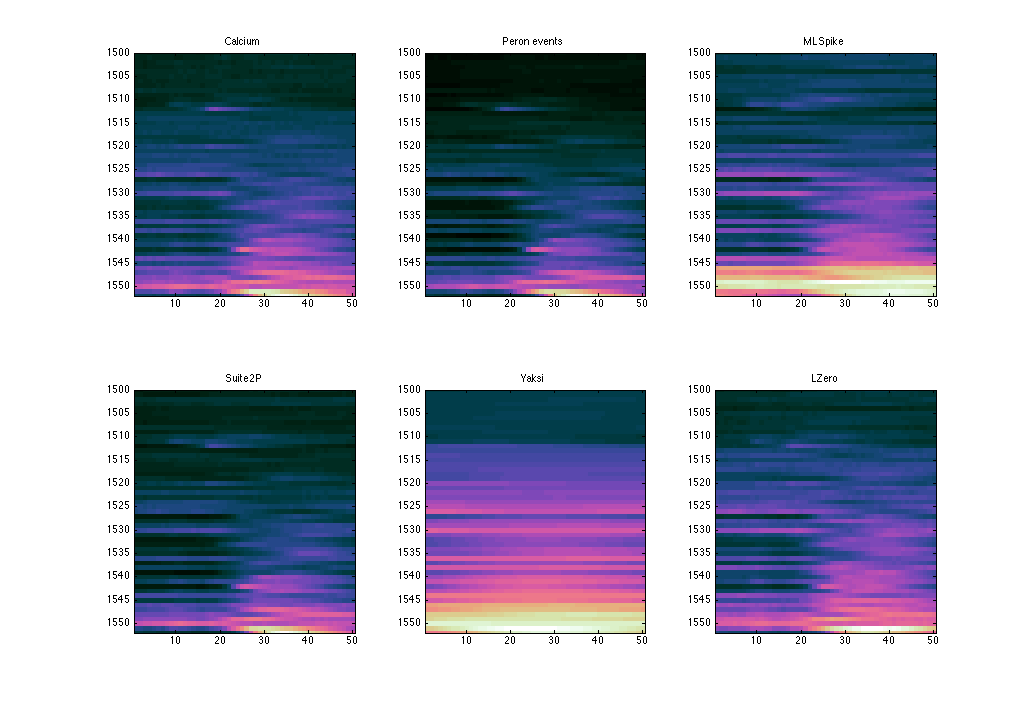
\includegraphics[width=1\textwidth]{psth_all_sorted_zoom2.png}
%\caption{\label{fig:PSTHs}PSTHs do not show increase in temporal sharpness following deconvolution.}
%\end{figure}





%We would expect to do a better job of distinguishing touch vs delay activity or delay vs reward. Is this true?


\section{Discussion}
\emph{MDH NOTES: Add a Discussion to collect notes on what the conclusions and recommendations are e.g.
(1) Don’t use PCC; use ER or something similar (full ROC)}

\emph{(1b) Deconvolution methods trade-off FNs vs FPs (hence need to use metric that captures both)}

PCC is invariant to affine transformations of the data (noted also by Theis et al). Therefore neither false positives nor false negatives are penalised per se, and spike inference results that maximise PCC between real and inferred spikes cannot be interpreted in terms of spike rate. If the goal of an analysis is to estimate the true firing rate or spike timing of the cell, PCC is not an appropriate metric to use in spike inference optimisation. Instead, a metric such as ER - which explicitly penalises both FPs and FNs, giving better scores to inferred spike trains that are closer to the true spike train in terms of spike count and timing - are a better choice.


\emph{(2) Choice of deconvolution method will change inferences taken from all analyses that follow. So use either (a) raw Ca2+ and deconvolution OR (b) two different deconvolution methods. [NB this links with ideas of robust inference: that obtaining the same result in the face of wide variation increases its reliability]}

\emph{(3) Message is *not* abandon deconvolution; message is: get it solved. We need these problems solved: when we move to very high frame rate imaging and faster Ca2 sensors, then we will want to look at neural coding at spike resolution. So we will need deconvolution to be properly reliable...}

Many questions do not require spike timing (see short discussion in Harris et al 2016 NN Review `Improving data quality in neuronal population recordings'). 

\clearpage
\section{Methods}

\subsection*{Spike train metrics}
Pearson correlation coefficient - down sampled or gaussian convolved.
Deneux implementation of normalised error rate, derived from Victor and Purpura 1996 Error Rate.


\subsection*{List of deconvolution methods}

\subsubsection*{Suite2P}
\texttt{Suite2P} (\href{https://github.com/cortex-lab/Suite2P}{https://github.com/cortex-lab/Suite2P}) is actively developed by  Marius Pachitariu and members of the cortexlab (Kenneth Harris and Matteo Carandini) at UCL. Suite2P's USP is it's application to large scale 2-photon imaging analysis, with an emphasis on end-to-end processing (images to neural event time series) and speed. A preprint describing the toolbox is available here:\\

\noindent \href{http://biorxiv.org/content/early/2016/06/30/061507}{http://biorxiv.org/content/early/2016/06/30/061507}, \\

\noindent and our own notes on the spike detection algorithm are here:\\

\noindent \href{https://drive.google.com/open?id=1NeQhmoRpS-x8R0e84w3TqkUR1PNMXiem6ZIjJta-U7A}{https://drive.google.com/open?id=1NeQhmoRpS-x8R0e84w3TqkUR1PNMXiem6ZIjJta-U7A}.

\subsubsection*{MLSpike}
\texttt{MLSpike} (\href{https://github.com/mlspike}{https://github.com/mlspike}) was developed by Thomas Deneux at INT, CRNS Marseille, France. A model-based probabilistic approach, \texttt{MLSpike} was developed to recover spike trains in calcium imaging data by taking baseline fluctuations and cellular properties into account. A comprehensive explanation of the algorithm and its benefits can be found in the paper:\\

\noindent Deneux, Thomas, Attila Kaszas, Gergely Szalay, Gergely Katona, Tamás Lakner, Amiram Grinvald, Balázs Rózsa, and Ivo Vanzetta. "Accurate spike estimation from noisy calcium signals for ultrafast three-dimensional imaging of large neuronal populations in vivo." Nature Communications 7 (2016).\\

\noindent Link: \href{https://www.nature.com/articles/ncomms12190}{https://www.nature.com/articles/ncomms12190}

MLSpike can return a maximum a posteriori spike train, or a spike probability per time step. We show results for both denoted MLSpike$_{events}$ and MLSpike$_{pspike}$

\subsubsection*{LZero}
The method we refer to as \texttt{LZero} was developed by Sean Jewell and Daniela Witten from U.Washington, Seatle, USA. The goal for this implementation was to cast spike detection as a change-point detection problem, which could be solved with an existing $l_{0}$ optimization algorithm. In their paper Jewell and Witten show that the $l_{0}$ solution is better than previously implemented $l_{2}$ solutions, with results much closer to the real spike train ($l_{2}$ solutions tend to overestimate the true firing rate). Details can be found in the paper:\\

\noindent Jewell, Sean, and Daniela Witten. "Exact Spike Train Inference Via $l_{0}$ Optimization." arXiv preprint arXiv:1703.08644 (2017).\\

\noindent Link: \href{https://arxiv.org/abs/1703.08644}{https://arxiv.org/abs/1703.08644}

\subsubsection*{Yaksi}
\texttt{Yaksi} refers to the `vanilla' deconvolution of Yaksi and Friedrich (2006). This is to be used as a baseline for comparison with more sophisticated methods. \st{\textbf{\emph{NOTE 8.6.17}} my implementation results in signals that are more temporally smooth (as opposed to more temporally sharp) than the calcium signal, indicating the filtering has not been performed properly.} \\

\noindent The method is detailed in the paper: \\
\noindent Yaksi, Emre, and Rainer W. Friedrich. "Reconstruction of firing rate changes across neuronal populations by temporally deconvolved Ca2+ imaging." Nature Methods 3, no. 5 (2006): 377-383.


\subsubsection*{Peron events}
\texttt{Peron events} refer to the extracted events detailed in the original \emph{Peron et al. 2015} paper. It is a version of the 'peeling' algorithm tuned to generate a low number of false positive detections (a rate of 0.01Hz) on ground truth data, leading to a hit rate of 54$\%$

\noindent Peron, Simon P., Jeremy Freeman, Vijay Iyer, Caiying Guo, and Karel Svoboda. "A cellular resolution map of barrel cortex activity during tactile behavior." Neuron 86, no. 3 (2015): 783-799.

\subsubsection*{Events + kernel versions}
Where a spike inference method returns spike rates per time point, these are plotted as Method$_{events}$. To compare to other methods that return a de-noised df/f or firing rate estimate, these events are convolved with a calcium kernel and plotted as Method$_{kernel}$.

\clearpage
\section{Supplemental}

\begin{figure}[h!]
\centering
\subfigure[]{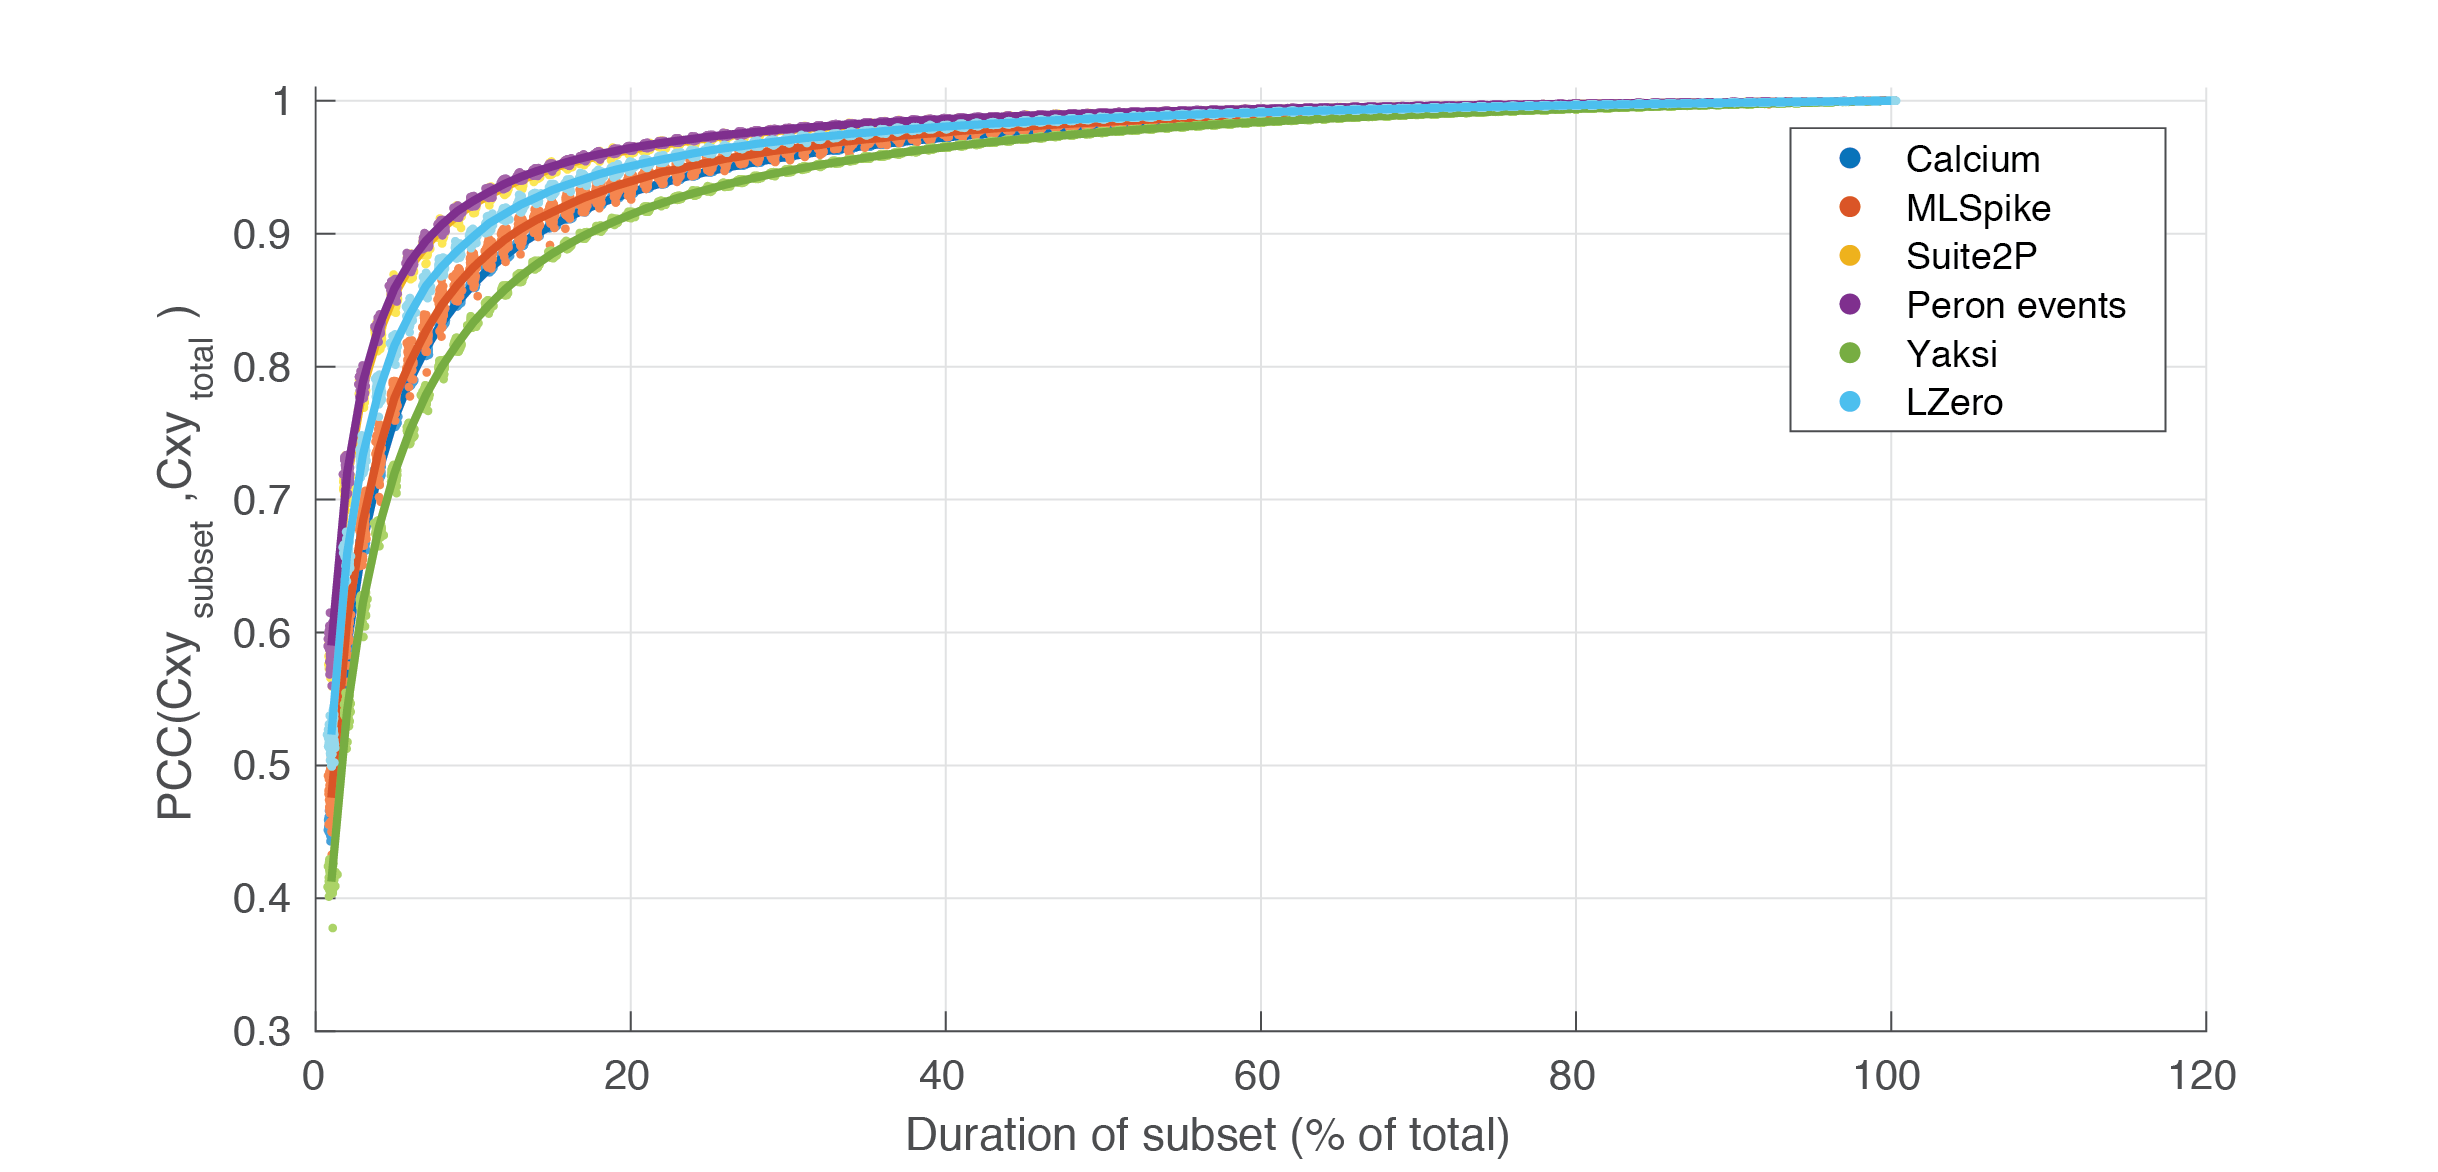
\includegraphics[trim={30 20 40 20},clip,width=0.6\textwidth]{figs/cxy_subset_comparison3.png}}%
\subfigure[]{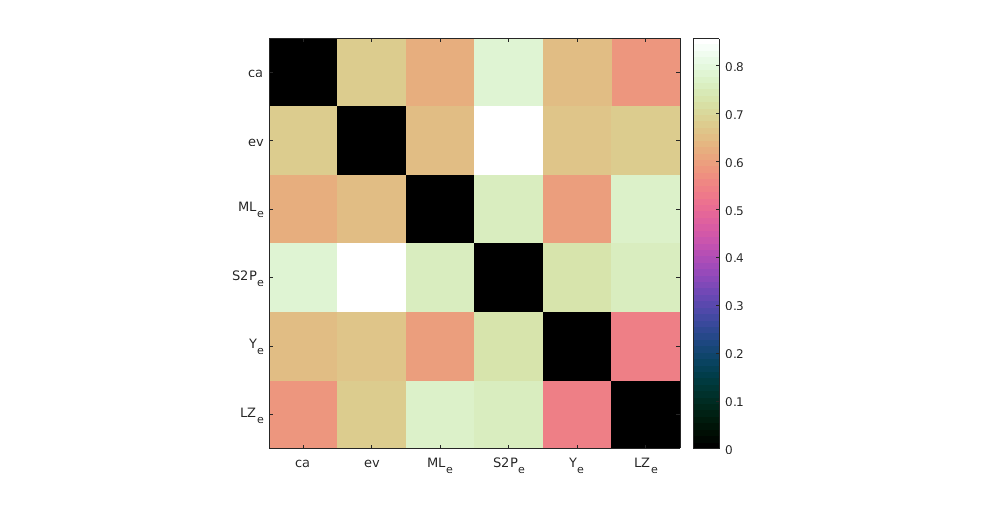
\includegraphics[trim={170 20 180 20},clip,width=0.3\textwidth]{figs/cxy_pcc_grid_cubehelix.png}}
\caption{\label{fig:supp_cxy_stability}Example datasets are long enough to generate stable correlation estimates. (a) Correlation between the pairwise correlation matrix for a given method, and an equivalent correlation matrix for subsets of the data. For each datapoint in the figure a subset (1\%-100\%) of the full dataset is extracted at random without replacement and a matrix of pairwise correlations is generated. These correlations are then compared to the matching pairwise correlations in the full dataset. In all instances 20\% of the data is sufficient to recover correlations of 0.9, though there is substantial variation between methods. (b) Pairwise correlation matrix between correlation matrices for each method.}
\end{figure} % Code for this plot is in compare_peron.m


\begin{figure}[h!]
\centering
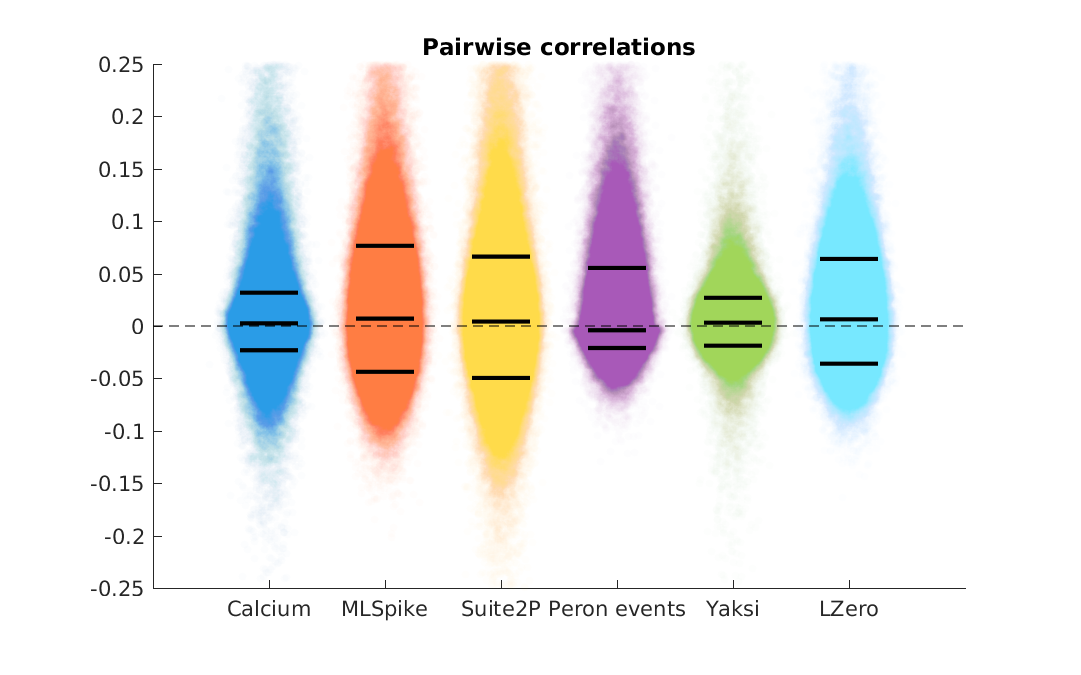
\includegraphics[width=0.9\textwidth]{pairwise_scatter3_alph_pt01_zoom.eps}
\caption{\label{fig:PCCs_zoom}Zoomed in version of \ref{fig:PCCs} }
\end{figure}

\begin{figure}[h!]
\centering
\subfigure{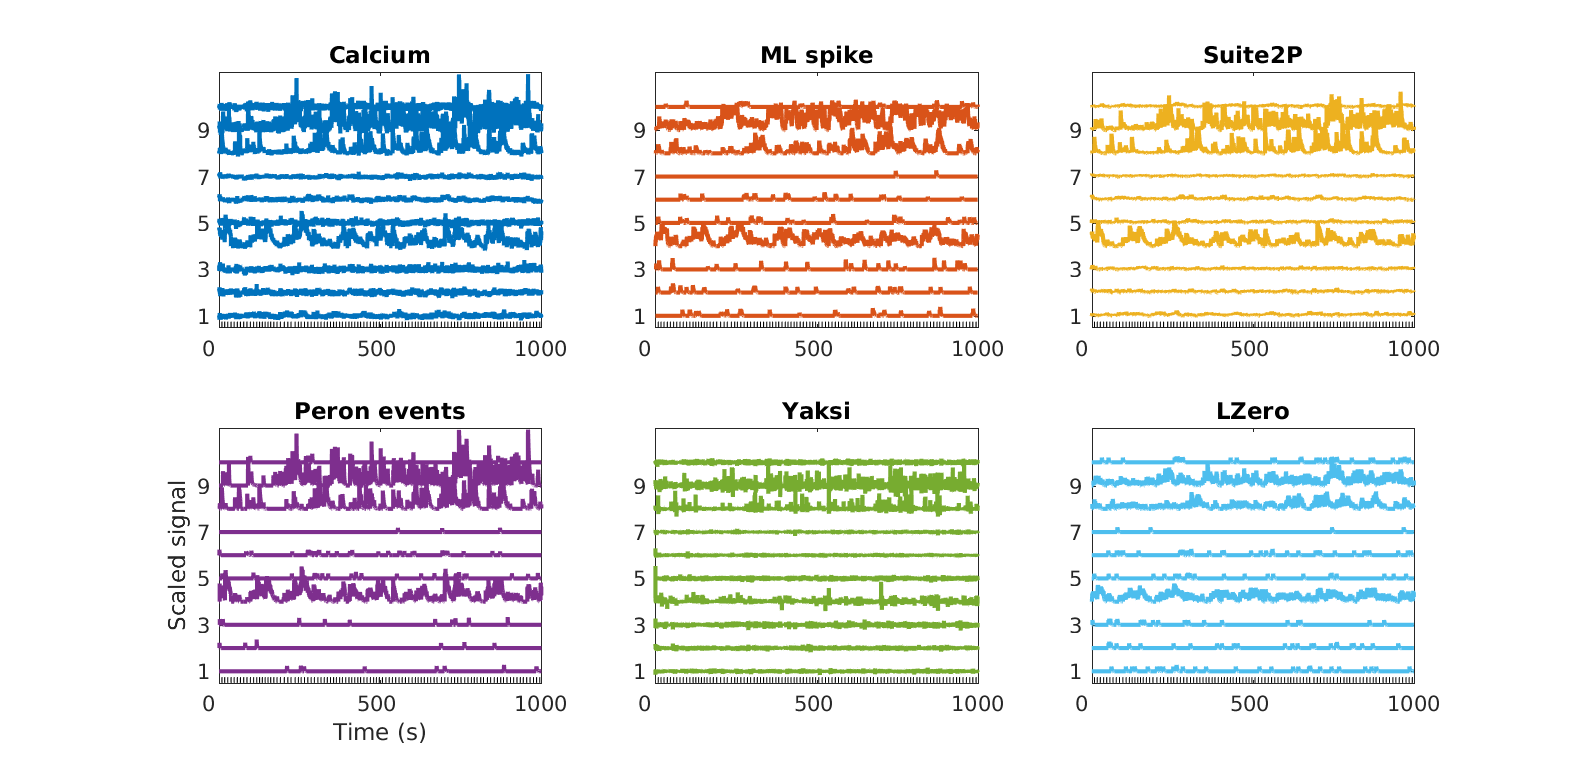
\includegraphics[width=0.9\textwidth]{10cells_compare2.eps}}
\subfigure{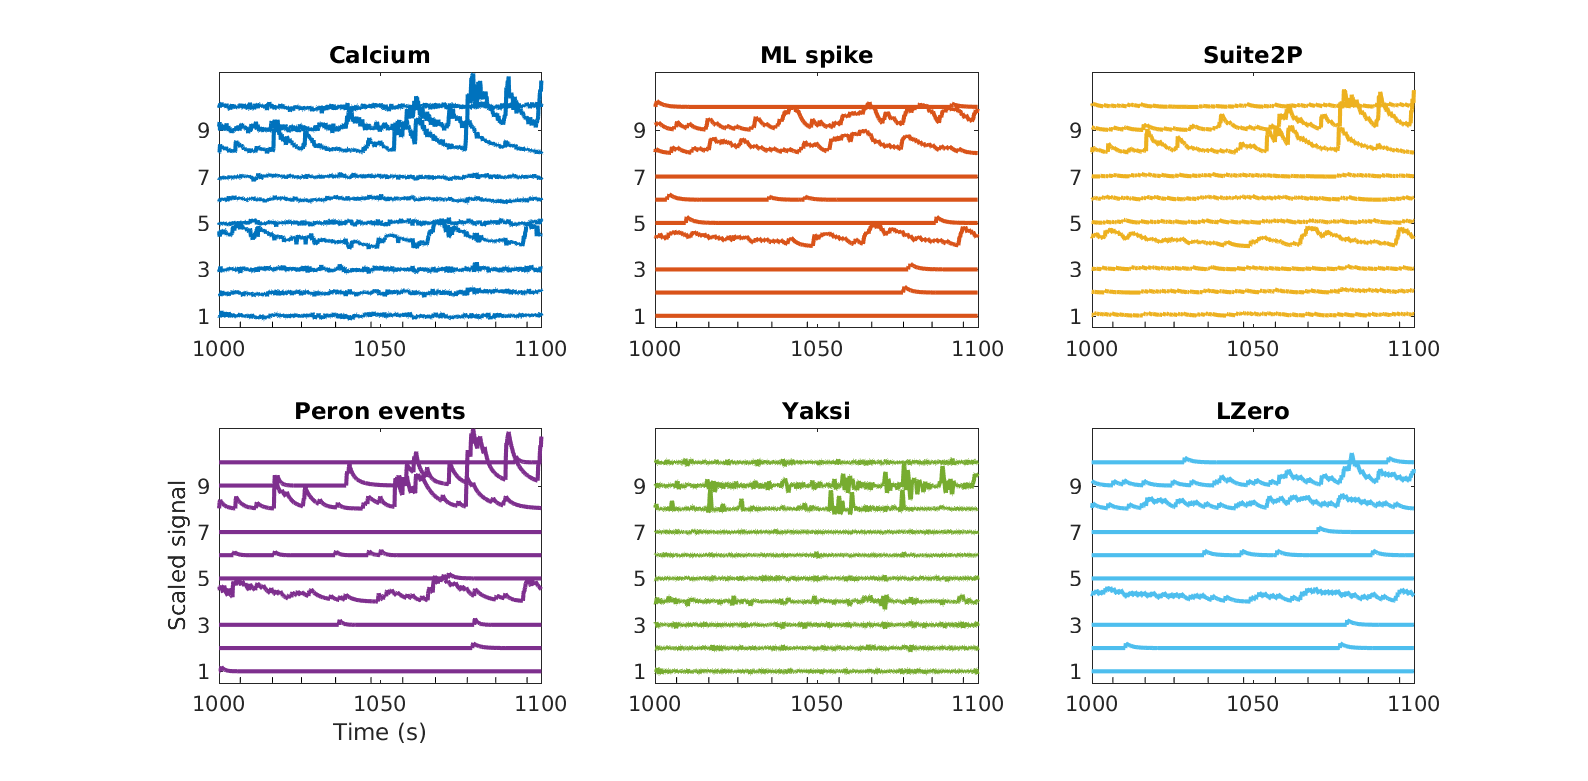
\includegraphics[width=0.9\textwidth]{10cells_compare2_zoom.eps}}
\subfigure{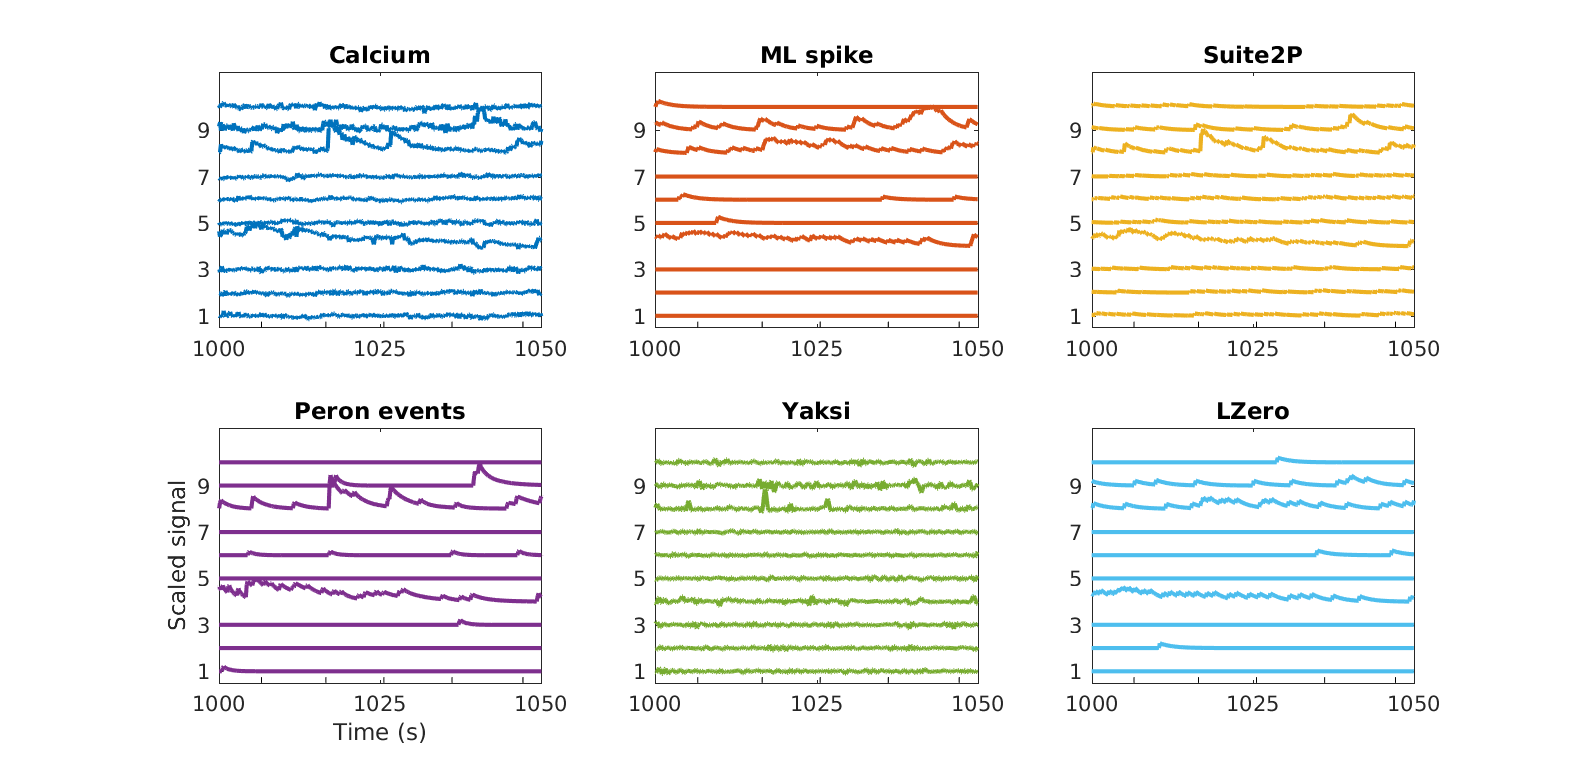
\includegraphics[width=0.9\textwidth]{10cells_compare2_zoom2.eps}}
\caption{\label{fig:raw1}Example deconvolution for 10 cells using each method. Different figures are the same data at increasing levels of zoom.}
\end{figure}

\begin{figure}[h!]
\centering
\subfigure{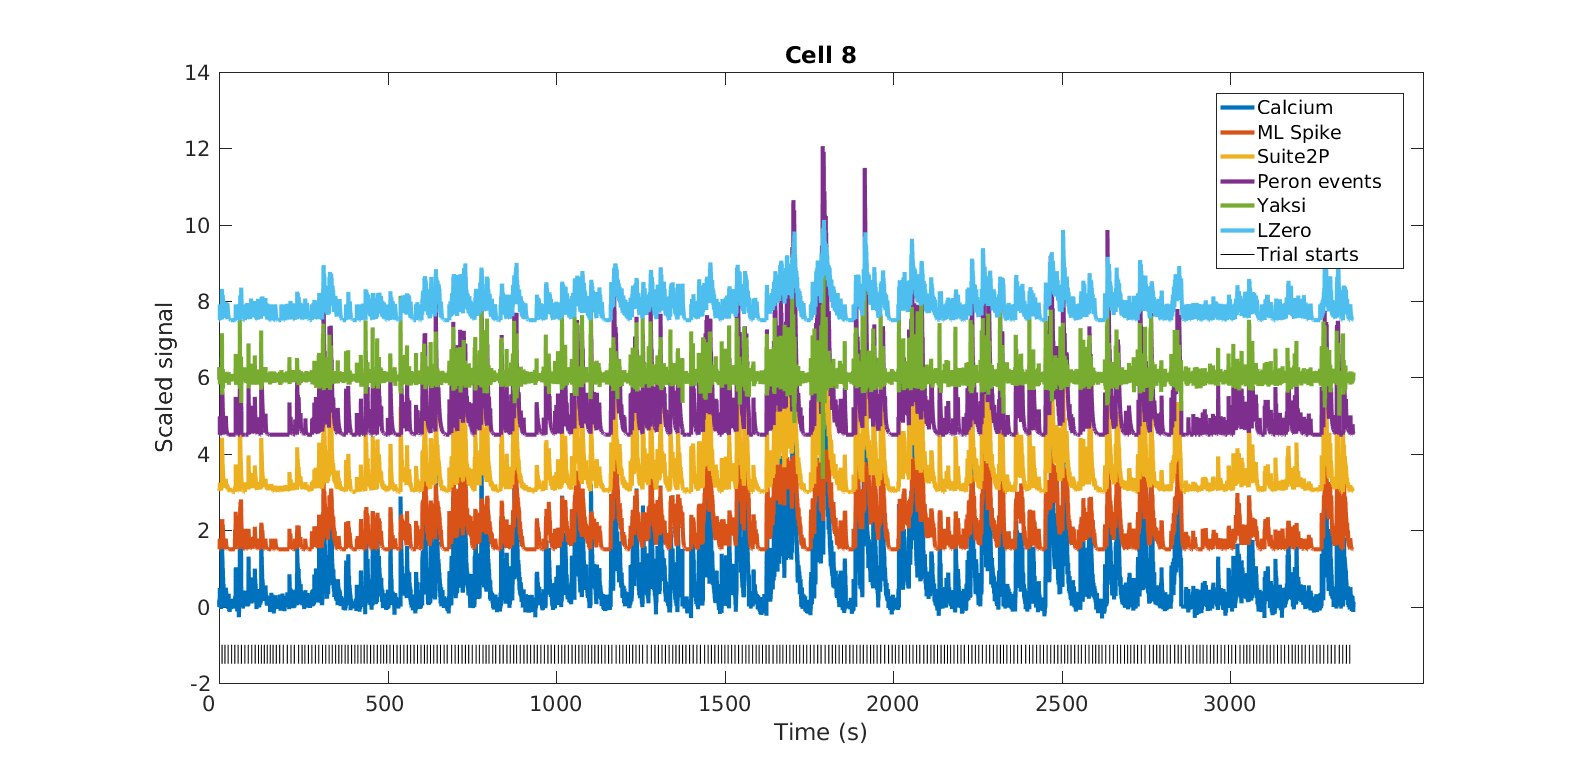
\includegraphics[width=0.75\textwidth]{cell8_deconv_compare2.eps}}
\subfigure{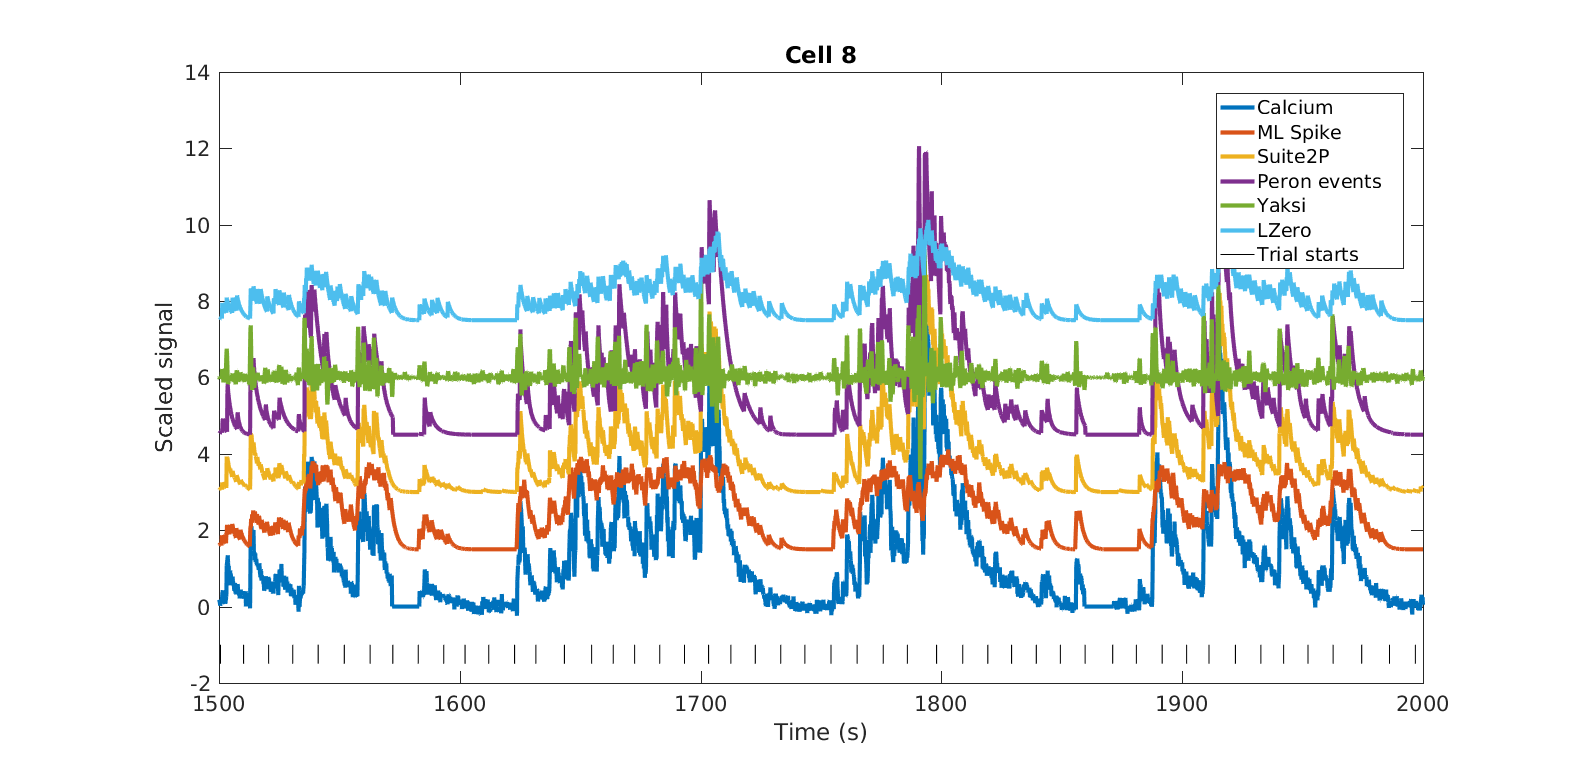
\includegraphics[width=0.75\textwidth]{cell8_deconv_compare2_zoom1.eps}}
\subfigure{\includegraphics[width=0.75\textwidth]{cell8_deconv_compare2_zoom2.eps}}
\subfigure{\includegraphics[width=0.75\textwidth]{cell8_deconv_compare2_zoom3.eps}}
\caption{\label{fig:raw1}Example deconvolution for one cell using each method. Different figures are the same data at increasing levels of zoom.}
\end{figure}



% \subsection{How to add Citations and a References List}

% You can upload a \verb|.bib| file containing your BibTeX entries, created with JabRef; or import your \href{https://www.overleaf.com/blog/184}{Mendeley}, CiteULike or Zotero library as a \verb|.bib| file. You can then cite entries from it, like this: \cite{greenwade93}. Just remember to specify a bibliography style, as well as the filename of the \verb|.bib|.

% You can find a \href{https://www.overleaf.com/help/97-how-to-include-a-bibliography-using-bibtex}{video tutorial here} to learn more about BibTeX.

% We hope you find Overleaf useful, and please let us know if you have any feedback using the help menu above --- or use the contact form at \url{https://www.overleaf.com/contact}!

% \bibliographystyle{alpha}
% \bibliography{sample}

\end{document}